\documentclass[11pt,a4paper]{article}
\usepackage[utf8]{inputenc}
\usepackage[margin=1in]{geometry}
\usepackage{amsmath,amssymb,amsthm,mathtools}
\usepackage{booktabs}
\usepackage{array}
\usepackage{graphicx}
\usepackage{float}
\usepackage{caption}
\usepackage{tikz}
\usetikzlibrary{arrows.meta,positioning,fit,patterns,calc,shapes.geometric}
\usepackage{algorithm}
\usepackage{algpseudocode}
\usepackage[hidelinks]{hyperref}
\usepackage{natbib}
\bibliographystyle{plainnat}
\usepackage[expansion=false]{microtype}
\usepackage{setspace}
\onehalfspacing
\setlength{\emergencystretch}{3em}

\theoremstyle{plain}
\newtheorem{proposition}{Proposition}
\newtheorem{corollary}[proposition]{Corollary}
\newtheorem{lemma}[proposition]{Lemma}
\theoremstyle{definition}
\newtheorem{definition}{Definition}
\newtheorem{remark}{Remark}
\theoremstyle{definition}
\newtheorem{example}{Example}
\theoremstyle{plain}
\newtheorem{assumption}{Assumption}

\DeclareMathOperator*{\argmax}{arg\,max}
\newcommand{\Prob}{\mathbb{P}}
\newcommand{\E}{\mathbb{E}}
\newcommand{\ind}[1]{\mathbf{1}\{#1\}}

\title{\bfseries Governing privacy risk across repeated statistical releases:\\
probability models, programme tolerances and accountable decisions}

\author{Ronald Rethabile Malamule Mahomane\thanks{Corresponding author:
\texttt{ron@basisenergygroup.com}. An earlier and shorter version was prepared for Session 5 of the Workshop on Data Security and Privacy, Banco de Portugal and Irving Fisher Committee, Lisbon, 14 and 15 September 2026. This is an author manuscript, not a BIS or IFC publication. Every
empirical table and quoted study result in this paper is produced by the
packaged pipeline in the companion repository; Section \ref{sec:repro} describes
what a run writes.}\\
\small Department of Computing, Mathematical and Statistical Sciences,
University of Namibia, Windhoek\\
\small School of Pathology, Faculty of Health Sciences,
University of the Witwatersrand, Johannesburg\\
\small Basis Energy, Victoria, Australia}

\date{Author manuscript: September 2026}

\begin{document}
\maketitle

\begin{abstract}
\noindent Central banks publish monthly from confidential registers, and an adversary can combine the vintages. We ask when a release programme, not a single release, is safe enough to publish, and who decides. Risk depends on a declared adversary and carries estimation error, so a decision should compare an upper confidence bound with a tolerance that has an owner, an expiry date, a harm class, a horizon, an error probability, a legal basis and an access route. With a persistent pseudonym, no function of per-release risks bounds a pooling adversary. On a synthetic credit register with six monthly vintages and a tolerance of 0.12, we choose the minimum cell count by fixed-sequence testing and confirm it on fresh targets. Per-release review passes the file with no suppression, or a floor of 20 when every firm size class must pass. An adversary who pools the vintages and knows when the target's loan is live needs 75 (200 for every size class). One who also holds an exposure reading per vintage needs 150, and no floor up to 200 protects every size class. No floor stops an insider who knows exposure closely. A floor of 150 keeps 20 per cent of loans, 4 per cent of exposure and no loan to a large firm. Against an adversary who knows loan histories, a loan-level release is the wrong product; aggregates or secure access are the realistic options. A neural network fitted to separate development attacks proposes the audit's bets and starting floor; it cut the attacks needed by about a fifth without changing the floor, and a logistic model did as well. Floors depend on the tolerance and on the adversary's reading precision. The results are synthetic.

\medskip\noindent\textbf{Keywords:} statistical disclosure control; record linkage; repeated releases; central bank statistics; risk tolerances; release governance.
\end{abstract}

\clearpage

\noindent\fbox{\parbox{.94\linewidth}{\textbf{Status.}
This is an author manuscript prepared for a central bank statistics audience and offered for consideration as an IFC Working Paper. It is not a BIS or IFC publication, and its views are the author's own. The companion journal article, ``Adaptive certification of attack-conditional disclosure risk across release programmes'', develops the sequential audit that Section \ref{sec:sequential} points to. An online appendix holds case studies from other data products and a neural procedure for proposing settings; neither enters the results.}}

\bigskip

\noindent\fbox{\parbox{.94\linewidth}{\setlength{\parskip}{4pt}\textbf{Executive summary.}

\textbf{Situation.} Central banks publish from confidential registers every month: aggregates, supervisory tables and, for accredited users, loan-level files. Each release is reviewed on its own, usually against a minimum cell count, and the review reports a point figure for the risk.

\textbf{Complication.} An adversary holds every vintage, not one. When records keep a pseudonym across releases, no function of the per-release risks bounds what that adversary can do (Proposition \ref{prop:nopool}). The risk figure is also an estimate, and a point estimate at the tolerance passes about half the time (Proposition \ref{prop:point}). Nobody owns the tolerance, and it has no expiry date.

\textbf{Question.} When is a release programme, rather than one release, safe enough to publish, who decides, and what does the answer cost in data?

\textbf{Answer.} Compare an exact upper bound on the programme's risk with a written tolerance that has an owner, an expiry date, a harm class, a horizon, a legal basis and an access route, and choose the protection level by fixed-sequence testing confirmed on fresh targets. On a synthetic credit register at a tolerance of 0.12, per-release review passes the loan-level file with no suppression (a floor of 20 if every firm size class must pass). An adversary who pools six vintages and knows when the target's loan is live needs a floor of 75 (200 for every size class); one who also reads exposure in each vintage needs 150, and no floor up to 200 protects every size class. No floor stops an insider who knows exposure closely. A floor of 150 keeps 20 per cent of loans, 4 per cent of exposure and no loan to a large firm (Table \ref{tab:robust}). Against an adversary who knows loan histories, a loan-level release is the wrong product: aggregates, or access in a secure setting under the Five Safes, are the realistic options. The loan-level file here stands in for securitisation loan-level disclosures and for research files as an accredited user sees them. The floors depend on the tolerance (Table \ref{tab:tolerance-floors}) and on how precisely the adversary reads exposure (Table \ref{tab:replication}). A neural network fitted to development attacks proposes the audit plan, and only fresh audit outcomes certify the floor (Section \ref{sec:eval-neural}).}}

\clearpage

{\setcounter{tocdepth}{2}\tableofcontents}

\clearpage

\section{Introduction}\label{sec:intro}

Central banks, statistical offices and health registries release granular data
under a statutory duty of confidentiality. The technical means of protection
are well developed. Cell suppression, minimum cell counts, global recoding,
record swapping, the cell-key method, additive noise, synthetic data and formal
privacy mechanisms are all documented, implemented and taught
\citep{willenborg1996,willenborg2001,duncanelliot2011,hundepool2012,templ2015,dwork2014}. The object that
remains underdeveloped is the decision rule that turns a measured risk into an
admissible or inadmissible release.

Practice usually settles this by committee. A disclosure control officer
presents a table of risk measures, a panel weighs them against the public value
of the release, and a decision follows. The decision is often sound. It is
rarely reproducible, and it is hard to audit after the fact, because the
deciding quantity, how much residual risk the institution was
willing to carry, was never written down. Improving the protection mechanism
does not repair this. A mechanism with a formal guarantee can still be governed
by an unstated tolerance, and an institution can adopt a carefully accounted $\varepsilon$ without being
able to say what probability of harm it accepted.

This paper separates three objects that are routinely run together.

\begin{enumerate}
\item A probability model for an adversary's attempted linkage, conditional on
a declared attack scenario.
\item A statistical estimate of the resulting risk, with its uncertainty.
\item A policy decision that states how much residual risk is acceptable, for
which harm class, on whose authority, and until when.
\end{enumerate}

The first is a modelling problem, the second an inference problem, the third a
governance problem. Confusing them produces two familiar failures. A committee
that releases whenever the point estimate falls below its tolerance will, for a
release whose true risk equals the tolerance, release with probability near one
half (Proposition \ref{prop:point}). An institution that treats a protection
parameter as a tolerance never states the probability it accepted.

\subsection{Contribution}

The paper makes four contributions.

First, we derive the prosecutor, journalist and marketer measures from a single
linkage experiment (Section \ref{sec:experiment}). The reciprocal-frequency
formula $1/f_k$ follows from four stated assumptions, as
\citet{duncan1989} and \citet{skinner2002} also show. Two of
those assumptions, exchangeability of the records sharing a key and error-free
observation of the key, fail whenever the adversary holds informative side
information, and then the posterior linkage probability exceeds $1/f_k$. The
same derivation gives $k$-anonymity its scope (Proposition \ref{prop:kanon}): on
a declared key it does not deliver $1/k$ when the intruder also knows a released
continuous variable. In the simulation of Section \ref{sec:sim}, a
10-anonymous release contains a record whose own re-identification probability
is 0.74, with a one-sided 95 per cent lower bound of 0.64.

Second, we treat the risk figure as an estimate that enters a written decision
rule (Sections \ref{sec:est} and \ref{sec:gov}). A release is admissible only
when an upper confidence bound, not a point estimate, lies below a tolerance
that has a named owner, an expiry date, a harm class, a declared adversary, a
stated error probability, a legal basis with the parties it protects, an access
route and, for a programme, a horizon. The rule has a price
(Proposition \ref{prop:cert}): certifying $\tau = 10^{-3}$ at the 5 per cent
level needs 2,995 independent attacks without a success, and $\tau = 10^{-5}$
needs 299,572. Supporting results sign the bias of plug-in frequency measures
(Proposition \ref{prop:plugin}), give the relative harm weight a tolerance
implies (Proposition \ref{prop:tau}, after \citet{abowd2019}), and relate
scenario risk to differential privacy (Proposition \ref{prop:dpbound}).

Third, we state what marginal risks can and cannot say about a release
programme. The sharp bounds from the marginals are $\max_i R_i \leq R_\cup \leq
\min(1, \sum_i R_i)$ (Proposition \ref{prop:boole}). When records carry a
pseudonym that is the same in every release, no bound on a pooling adversary in
terms of the marginals exists (Proposition \ref{prop:nopool}). The construction
is the classic intersection attack \citep{sweeney2002,ganta2008}, and with a
persistent pseudonym the programme is one release keyed on the union of the
keys, so the result says that a finer key can carry far more risk than any of
its projections (Remark \ref{rem:finer}). What we add is its statement in the
terms a certifying body uses.

Fourth, we evaluate the rule on a synthetic credit register built to share the
structure of a supervisory collection (Section \ref{sec:eval}). Loans enter and
leave the register over six monthly vintages, and the same adversary faces five
loan-level protection policies. The minimum cell count is chosen by
fixed-sequence testing on the upper bound and confirmed on a second draw of
targets (Table \ref{tab:robust}). At a tolerance of 0.12, per-release review
passes the file with no suppression, or with a floor of 20 when every firm size
class must meet the tolerance. An adversary who pools the vintages and knows in
which of them the target's loan is live needs a floor of 75, or 200 for every
size class. Without that knowledge pooling adds nothing on this register
(Proposition \ref{prop:nohistory}). An adversary who also holds one exposure
reading per vintage needs 150, and no floor up to 200 protects every size class.
No floor up to 300 stops an insider who reads exposure with small error. The cost
falls on credit volume more than on loan counts: the floor of 150 keeps 20 per
cent of loans but 4 per cent of exposure, and no loan to a large firm. Against an
adversary who knows loan histories, then, a loan-level release is the wrong
product, and aggregates or access in a secure setting are the realistic options.
The floors are conditional on the tolerance (Table \ref{tab:tolerance-floors})
and on how precisely the adversary reads exposure (Table \ref{tab:replication}).
Rotating the pseudonym does not help while exposure is published exactly,
because the published key and exposure relink every loan; with exposure rounded
to one significant figure they relink about one loan in ten.

\subsection{Reader's guide}

A reader at a central bank who wants to apply the paper to its own releases
should start with Section \ref{sec:apply}. It sets out seven steps, the roles
they need, starting declarations for six release types common in central banks
(Table \ref{tab:apply-map}), the remedies to use when a release fails and a
small pilot, and Appendix \ref{app:worksheets} holds blank worksheets for each
step. A reader who wants the recommendation and its evidence can read three
parts. Section \ref{sec:gov} states the governance rule. Section
\ref{sec:credit} describes the synthetic credit register and its five harms, and
Section \ref{sec:eval} runs the attack evaluation on it. Section
\ref{sec:protocol} gives the protocol and a filled decision record for the
register (Table \ref{tab:record}). The other sections supply the derivations
(Sections \ref{sec:setup} to \ref{sec:comp}), certification under monitoring
(Section \ref{sec:sequential}), the relation to formal privacy (Section
\ref{sec:dp}), a simulation on a synthetic population (Section \ref{sec:sim}),
two public microdata files (Section \ref{sec:real}) and six falsification tests
(Section \ref{sec:falsify}). Section \ref{sec:worked} gives worked examples of each step with the
paper's own numbers. Section \ref{sec:security} states, in the terms of
a security evaluation, what the method adds to a release system and what it
does not, and Section \ref{sec:conclusion} concludes. The appendices hold the
proofs, expanded derivations, simulation details and the worksheets. Case
studies from other data products, and the earlier neural procedure SENTRY-R with its
proofs, are in a separate online appendix. The neural release pipeline that proposes
bets and a start floor for the audit is part of the main results (Section
\ref{sec:eval-neural}).

\subsection{Relation to existing work}\label{sec:lit}

The measurement literature is long and we do not restate it. Disclosure risk as
a probability conditional on an intruder scenario goes back to
\citet{duncan1989} and \citet{elliot1999}; per-record
and uniqueness measures and their estimation under a population-frequency model
are developed in \citet{skinnerholmes1998}, \citet{skinner2002},
\citet{reiter2005} and \citet{skinner2008}, with smoothing models by
\citet{rinott2006} and earlier by \citet{bethlehem1990}. \citet{elamir2004}
and \citet{franconi2004} estimate per-record risk from log-linear and
superpopulation models, and \citet{shlomoskinner2010} extend the estimation to
files perturbed by misclassification. The prosecutor,
journalist and marketer scenarios are named in \citet{elemam2008}.
\citet{skinner2012} separates the potential for disclosure from the harm it
causes, the distinction this paper keeps through the harm class of Section
\ref{sec:gov}. Record linkage under error is \citet{fellegi1969}. The risk--utility trade-off
was formalised as a map by \citet{duncan2001}, with utility measures developed
by \citet{karr2006}, \citet{woo2009} and \citet{snoke2018}.
\citet{trottini2002} model the user's uncertainty on both axes of the map, and
\citet{gomatam2005} apply it to remote analysis servers that release query
answers instead of microdata. \citet{stadler2022} tested synthetic data, which
\citet{drechsler2011} sets out as a release strategy, against inference attacks
and found that it either left the attacks open or lost utility, and that the
outcome varied from one dataset to the next. Formal privacy
begins with \citet{dinur2003} and \citet{dwork2006a,dwork2006b}, and
\citet{mcsherry2007} extend it from numeric answers to general outputs, with the
composition and accounting machinery in \citet{dwork2010}, \citet{kairouz2017},
\citet{dwork2014},
\citet{bun2016}, \citet{mironov2017} and \citet{dong2022}, and the statistical
reading in \citet{wasserman2010} and \citet{duchi2018}. The economic reading of
the trade-off as a social choice is \citet{abowd2019}, with the census
application in \citet{abowd2022} and the counterargument in \citet{hotz2022}.
The governance literature, in particular the Five Safes
\citep{desai2016} and the anonymisation decision-making framework
\citep{elliot2020}, is where tolerances and accountability are discussed, and it
is largely disjoint from the measurement literature.

Three of this paper's components have close antecedents, and we state what is
taken from them. The result that a tolerance is pinned by the
relative harm weight assigned to disclosure risk and public value is a restatement,
in a per-release governance setting, of the social-choice argument of
\citet{abowd2019}; the economics is theirs and the contribution here is only to
carry it into a decision rule that a release committee can operate. The threshold
at which an adversary acts follows from its payoffs rather than from the
convention of one half, which is the premise of the game-theoretic analyses of
re-identification risk \citep{wan2015}; what is added is the requirement that an
evaluation report the precision and coverage curve over that threshold rather
than one point on it. And the anytime-valid machinery of Section
\ref{sec:sequential} is standard: the martingale bound is \citet{ville1939}, the
modern confidence sequences are \citet{howard2021}, and the framework is set out
in \citet{ramdas2023}, with the adaptive-analysis problem in its statistical form
in \citet{dwork2015}. The contribution is the application, which is to certify a
disclosure risk while the simulation is being monitored, and the measurement of
what monitoring costs.

The two bodies of work are not joined. The measurement literature produces
numbers without saying which decision they license; the governance literature
produces accountability structures without saying which number triggers them. Two specific gaps motivate this paper. The first is not the
variance of a risk estimate: \citet{skinner2008} and \citet{rinott2006} give
variance and interval estimates for per-record and file-level risk under
population-frequency models, and \citet{brown2001} and the exact binomial
interval of \citet{clopper1934} give the tools for simulated risk. What is
missing is a decision rule that uses an upper bound rather than a point
estimate, names an owner and an expiry date, and states whether it covers one
release or a programme. The second is that neither literature states
what a programme of releases may claim, as opposed to a single release, once the
adversary is allowed to combine them, though the reconstruction attacks of
\citet{dinur2003}, \citet{garfinkel2019} and \citet{dick2023} and the
de-anonymisation work of \citet{narayanan2008} and \citet{rocher2019} show that
combination is the operative threat. The evidence that a few attributes single
people out is older. \citet{sweeney2000} and \citet{golle2006} found that date
of birth, sex and postcode identify most of the US population, and
\citet{demontjoye2013,demontjoye2015} found that four points in space and time
identify nine in ten people in mobile phone and card payment records. A review
of published attacks on health data \citep{elemam2011} found that most were
small and targeted data that had not been de-identified to any standard, which
is a reason to report the adversary with the risk figure.

\section{Population, sample, keys and mechanisms}\label{sec:setup}

Let the finite population be $P = \{1, \dots, N\}$. A confidential sample is
indexed by the random set $I \subseteq P$ with $|I| = n$. Its inclusion
indicators and first-order inclusion probabilities are
\begin{equation}
S_i = \ind{i \in I}, \qquad \pi_i = \Prob(S_i = 1), \qquad i \in P .
\end{equation}
Under simple random sampling without replacement, $\pi_i = n/N$ for every $i$;
under Bernoulli sampling the $S_i$ are independent with common $\pi$. A census
is the limiting case $I = P$ and $\pi_i = 1$.

Let $X_i \in \mathcal{X}$ be the confidential record of unit $i$. An adversary
does not necessarily observe all of $X_i$. It uses a declared key map
\begin{equation}
K_a : \mathcal{X} \longrightarrow \mathcal{K}_a ,
\end{equation}
where the subscript $a$ records the assumed attack scenario. For $k \in
\mathcal{K}_a$, define the population and sample key frequencies
\begin{equation}
F_k = \sum_{i \in P} \ind{K_a(X_i) = k}, \qquad
f_k = \sum_{i \in P} S_i \ind{K_a(X_i) = k} .
\label{eq:freq}
\end{equation}
Thus $0 \leq f_k \leq F_k$. The statements ``sample unique'' and ``population
unique'' mean $f_k = 1$ and $F_k = 1$.

A protection mechanism is a Markov kernel $M_\theta(dy \mid x)$ indexed by
$\theta \in \Theta$. The notation covers deterministic transformations as the
degenerate case. Applied to the confidential sample $X_I = (X_i : i \in I)$, it
generates a release
\begin{equation}
Y_\theta \sim M_\theta(\,\cdot \mid X_I) .
\label{eq:mech}
\end{equation}
The randomness in \eqref{eq:mech} matters for everything that follows. Risk is
a probability over four sources at once: the sampling design, the mechanism, the
noisy or incomplete auxiliary information held by the adversary, and any
randomisation in the adversary's own decision rule. An assessment that
integrates over some of these and conditions on others must say which.

\begin{remark}
Nothing in this section requires $\theta$ to carry a formal guarantee. A
minimum cell count of five, a coarser age classification and a Laplace mechanism
with $\varepsilon = 1$ are all points in $\Theta$. Section \ref{sec:dp} explains
why the last of these supports a claim the others do not, and why that claim is
not a linkage probability.
\end{remark}

\section{A unified linkage experiment}\label{sec:experiment}

Fix a target $t \in P$. The adversary observes auxiliary information $Z_t$ and
the release $Y_\theta$, then applies a measurable linkage rule
\begin{equation}
\delta_a : \mathcal{Z} \times \mathcal{Y} \longrightarrow I \cup \{\emptyset\} .
\label{eq:rule}
\end{equation}
The value $\delta_a(Z_t, Y_\theta) = j$ asserts that released record $j$
belongs to $t$, and $\emptyset$ denotes abstention. Correct identification is
the event
\begin{equation}
C_t(\theta, a) = \{S_t = 1, \ \delta_a(Z_t, Y_\theta) = t\} .
\end{equation}

\begin{definition}[Scenario-conditional target risk]\label{def:risk}
Given background information $\mathcal{B}_a$ declared by scenario $a$, the unconditional
and file-membership-conditional risks are
\begin{equation}
R_a^{\mathrm{unc}}(t, \theta) = \Prob\{C_t(\theta, a) \mid \mathcal{B}_a\}, \qquad
R_a^{\mathrm{in}}(t, \theta) = \Prob\{\delta_a(Z_t, Y_\theta) = t \mid S_t = 1,
\mathcal{B}_a\} .
\label{eq:tworisks}
\end{equation}
\end{definition}

The distinction in \eqref{eq:tworisks} prevents a common error. If membership
in the file is not known to the adversary, the unconditional risk carries an
inclusion-probability factor,
\begin{equation}
R_a^{\mathrm{unc}}(t, \theta) = \pi_t \, R_a^{\mathrm{in}}(t, \theta) ,
\label{eq:factor}
\end{equation}
provided a correct association is impossible when $S_t = 0$. Equation
\eqref{eq:factor} is the multiplication rule $\Prob(A \cap B) = \Prob(A \mid
B)\Prob(B)$ and not an independence assumption. Reporting the two quantities
under one label, which happens whenever a sampling fraction is quietly applied
or quietly omitted, changes the reported risk by an order of magnitude in the
simulation of Section \ref{sec:sim}.

\subsection{Exact matching as a special case}

Consider four assumptions.

\begin{assumption}\label{as:key}
The released key is unperturbed: $K_a$ applied to the release agrees with $K_a$
applied to the confidential sample.
\end{assumption}
\begin{assumption}\label{as:obs}
The adversary observes the target's key without error.
\end{assumption}
\begin{assumption}\label{as:exch}
All records sharing the target's key are exchangeable in the adversary's
information.
\end{assumption}
\begin{assumption}\label{as:unif}
The adversary selects uniformly among the compatible records.
\end{assumption}

\begin{proposition}[Reciprocal frequency]\label{prop:recip}
Under Assumptions \ref{as:key} to \ref{as:unif}, conditional on $S_t = 1$ and
$K_a(X_t) = k$,
\begin{equation}
\Prob\{\delta_a = t \mid S_t = 1, K_a(X_t) = k, f_k\} = \frac{1}{f_k} .
\label{eq:recip}
\end{equation}
\end{proposition}

\begin{proof}
See Appendix \ref{app:proofs}.
\end{proof}

Proposition \ref{prop:recip} states the assumptions behind a familiar formula
\citep{duncan1989,skinner2002}. Once they are stated, they can fail,
and two of them fail often. Assumption \ref{as:exch} fails whenever the
adversary holds a covariate correlated with the confidential variable, which is
the normal case in financial and health data. Assumption \ref{as:obs} fails
whenever the adversary's auxiliary source has reporting error, which is also the
normal case.

\subsection{Imperfect matching and posterior linkage probability}

For perturbed keys or measurement error, let $L_{tj}$ denote the likelihood of
the observed auxiliary information and released record $j$ under the hypothesis
$H_{tj}$ that $j$ belongs to $t$, in the sense of \citet{fellegi1969}. With
prior match weights $q_{tj}$ and a no-match hypothesis $H_{t0}$, Bayes' rule
gives
\begin{equation}
p_{tj} := \Prob(H_{tj} \mid Z_t, Y_\theta, \mathcal{B}_a)
= \frac{q_{tj} L_{tj}}{q_{t0} L_{t0} + \sum_{\ell \in I} q_{t\ell} L_{t\ell}} .
\label{eq:post}
\end{equation}
If the adversary chooses the maximum-posterior candidate, its conditional
success probability is
\begin{equation}
R_a^{\mathrm{in}}(t, \theta) = \E\Big[ \max_{j \in I} p_{tj} \ \Big| \ S_t = 1,
\mathcal{B}_a \Big] .
\label{eq:maxpost}
\end{equation}
When the only compatible records have equal likelihood and the no-match prior
is zero, \eqref{eq:post} and \eqref{eq:maxpost} reduce to \eqref{eq:recip}.
Measurement error therefore cannot be declared to reduce risk. It changes the
likelihood ratios, and it may either spread posterior mass across candidates or
concentrate it on one. Section \ref{sec:sim} exhibits a case where key
reporting error lowers success from 0.4663 to 0.3812 while one noisy continuous
covariate returns it to 0.4642, so that the reciprocal-frequency figure was
right by cancellation rather than by argument.

\subsection{The three conventional scenarios}\label{sec:three}

\paragraph{Prosecutor.}
The prosecutor knows $S_t = 1$. Under exact exchangeable matching,
\begin{equation}
R_{\mathrm{pros}}(t, \theta) = \frac{1}{f_{K_a(X_t)}} ,
\label{eq:pros}
\end{equation}
and a file-level conservative summary is the maximum target risk
\begin{equation}
R_{\max}(\theta) = \max_{i \in I} R_{\mathrm{pros}}(i, \theta) ,
\label{eq:max}
\end{equation}
or the whole empirical risk distribution, which is more informative and no
harder to publish. Calling \eqref{eq:pros} an upper bound over all conceivable
scenarios requires Assumptions \ref{as:obs} to \ref{as:unif}. An adversary with
identifying side information breaks exchangeability and can achieve a posterior
above $1/f_k$.

\paragraph{Journalist.}
The journalist does not know that the target is in the file. For a
sample-unique released record with key $k$, the classical object is
$\rho_k = \Prob(F_k = 1 \mid f_k = 1)$, the probability that a sample unique is
population unique \citep{skinnerholmes1998,skinner2002}. It is not the
journalist's linkage success, which for a sample unique is
$\E[1/F_k \mid f_k = 1] \geq \rho_k$, and it differs again from the journalist
risk $1/\min_k F_k$ of \citet{elemam2008}. We keep the name $\rho_k$ for the
uniqueness probability throughout. Bayes' theorem gives
\begin{equation}
\rho_k = \frac{\Prob(f_k = 1 \mid F_k = 1)\Prob(F_k = 1)}
{\sum_{v \geq 1}\Prob(f_k = 1 \mid F_k = v)\Prob(F_k = v)} .
\label{eq:journ}
\end{equation}
Under Bernoulli sampling with common inclusion probability $\pi = n/N$,
\begin{equation}
\Prob(f_k = 1 \mid F_k = v) = \binom{v}{1}\pi(1-\pi)^{v-1} ,
\label{eq:binom}
\end{equation}
and substitution into \eqref{eq:journ} yields
\begin{equation}
\rho_k = \frac{\pi \Prob(F_k = 1)}
{\sum_{v \geq 1} v\pi(1-\pi)^{v-1}\Prob(F_k = v)} .
\label{eq:rho}
\end{equation}
Equation \eqref{eq:rho} shows why the sampling fraction matters, and it shows
that $\pi$ alone is not enough: the calculation needs a model or external
evidence for the population frequency distribution
\citep{skinner2002,reiter2005,rinott2006}. Section \ref{sec:sim} reports what
that model costs. Using $\pi$ itself in place of $\rho$ overstates the truth
by a factor of about two at $\pi = 0.05$, while a fitted negative binomial frequency model, which is closed under
binomial thinning and therefore identified from the sample, is accurate to within 8 to
25 per cent.

\paragraph{Marketer.}
The marketer attacks many targets and values the expected fraction correctly
linked. If the attacked unit $J$ is drawn uniformly from the population,
\begin{equation}
R_{\mathrm{mark}}^{\mathrm{pop}}(\theta) = \frac{1}{N}\sum_{i \in P}
R_a^{\mathrm{unc}}(i, \theta) .
\label{eq:markpop}
\end{equation}
If instead one conditions on attacking the released records, and exact
exchangeable matching holds, the sample mean is
\begin{equation}
R_{\mathrm{mark}}^{\mathrm{sample}}(\theta)
= \frac{1}{n}\sum_{i \in I}\frac{1}{f_{K_a(X_i)}}
= \frac{1}{n}\sum_{k : f_k > 0} 1
= \frac{D_I}{n} ,
\label{eq:marksamp}
\end{equation}
where $D_I$ is the number of distinct released keys, because each occupied
class contributes $f_k \cdot (1/f_k) = 1$. Formula \eqref{eq:marksamp} is not
$n^{-1}\sum_i 1/F_{K(i)}$. The former models choice among released candidates;
the latter presumes population frequencies are known and describes a different
experiment. The attack population and the conditioning event belong beside any
marketer figure. In the simulation the sample-frequency
measure is 7.3 times the population-frequency version, and the unconditional
measure \eqref{eq:markpop} is smaller than both, at 0.023 against 0.466 and
0.064.

\subsection{$k$-anonymity is a threshold statement}

\begin{proposition}[$k$-anonymity as a decision rule]\label{prop:kanon}
Under Assumptions \ref{as:key} to \ref{as:unif}, for $\tau \in (0,1]$,
\begin{equation}
\sup_{t \in I} R_{\mathrm{pros}}(t, \theta) \leq \tau
\quad \Longleftrightarrow \quad
\min_{k : f_k > 0} f_k \geq \lceil 1/\tau \rceil ,
\end{equation}
so the release satisfies $k$-anonymity with $k = \lceil 1/\tau \rceil$ in the
sense of \citet{sweeney2002}. If Assumption \ref{as:exch} fails, for instance
because the release publishes a continuous variable of which the adversary holds
a noisy reading, the implication from right to left fails: there are releases
that are $k$-anonymous on the declared key for which
$\sup_t R_a^{\mathrm{in}}(t,\theta) > 1/k$.
\end{proposition}

\begin{proof}
See Appendix \ref{app:proofs}. The failure claim is constructive and is shown numerically in Section
\ref{sec:kanon}.
\end{proof}

Proposition \ref{prop:kanon} gives $k$-anonymity its scope. The failure it
describes is one of key selection: a release that is $k$-anonymous on a key that
leaves out a variable the intruder knows is not $k$-anonymous in the sense of
\citet{sweeney2002} \citep[ch.~3]{hundepool2012}. Read this way, $k$-anonymity is
the special case of the decision rule
\eqref{eq:admiss} below in which the risk model is exact exchangeable matching,
the estimate carries no uncertainty, and the tolerance is the reciprocal of an
integer. Each of those three simplifications is a place where an institution
can be wrong, and the third is the only one that is a policy choice. The same
reading applies to the syntactic strengthenings of $k$-anonymity, such as
$\ell$-diversity \citep{machanavajjhala2007} and $t$-closeness
\citep{li2007}: they restrict the attribute distribution within a key class
rather than the tolerance, and so they change the risk model, not the decision
rule.

\section{Estimation and statistical uncertainty}\label{sec:est}

The risk in Definition \ref{def:risk} is unknown. It is a functional of the
sampling design, the mechanism, the population frequency structure and the
adversary's information, and in any realistic scenario it has no closed form.
It must be estimated, and the estimate must carry its uncertainty into the
decision.

\subsection{Simulation estimator}

Let $D^{(1)}, \dots, D^{(B)}$ be attack simulations generated under the
declared scenario, and set $C_t^{(b)} = 1$ if replicate $b$ identifies $t$
correctly. The Monte Carlo estimator is
\begin{equation}
\widehat{R}_a(t, \theta) = \frac{1}{B}\sum_{b=1}^{B} C_t^{(b)},
\qquad
\E[\widehat{R}_a] = R_a, \qquad
\mathrm{Var}(\widehat{R}_a) = \frac{R_a(1 - R_a)}{B} ,
\label{eq:mc}
\end{equation}
the variance holding because the $C_t^{(b)}$ are independent Bernoulli
variables under independent simulation. If replicates share auxiliary data,
records or fitted parameters, independence fails and \eqref{eq:mc} understates
the variance. The remedy is a clustered bootstrap over the shared unit, a
posterior interval, or a repeated-sample calculation that preserves the
dependence. The clustered version resamples whole units of sharing, the
auxiliary file or the fitted parameter draw, rather than individual attacks, and
recomputes the risk within each resampled cluster
\citep{efron1993,vandervaart1998}; the between-cluster spread then carries the
dependence that \eqref{eq:mc} assumes away. The nested design of Section
\ref{sec:nested} is the same accounting written as an analysis of variance, and
either device answers the same question: how much of the reported precision comes
from the number of simulated attacks alone. Institutions that reuse one auxiliary
file across all replicates are in this case and should not quote
\eqref{eq:mc}.

\subsection{Small risks and the zero-success problem}

For small risks a normal interval is unreliable \citep{brown2001}. An exact or
score-based one-sided bound $\overline{R}_{1-\alpha}$ should be reported. With zero
successes in $B$ independent simulations, the one-sided Clopper--Pearson bound
\citep{clopper1934} solves $(1 - U)^B = \alpha$, so
\begin{equation}
\overline{R}_{1-\alpha} = 1 - \alpha^{1/B} \approx -\frac{\log \alpha}{B} .
\label{eq:cp0}
\end{equation}
At 95 per cent confidence this is approximately $3/B$, the rule of three of
\citet{hanley1983}. Observing no successful
attack does not establish zero risk, and the strength of the statement is set
entirely by $B$.

\begin{proposition}[Certification cost]\label{prop:cert}
Suppose $B$ independent simulated attacks produce no success. The one-sided
$(1-\alpha)$ bound satisfies $\overline{R}_{1-\alpha} \leq \tau$ if and only if
\begin{equation}
B \geq \frac{\log \alpha}{\log(1 - \tau)} \approx \frac{-\log\alpha}{\tau}
\quad \text{as } \tau \downarrow 0 .
\label{eq:cert}
\end{equation}
\end{proposition}

\begin{proof}
See Appendix \ref{app:proofs}.
\end{proof}

The practical content of \eqref{eq:cert} is a budget. Certifying $\tau = 0.01$
at $\alpha = 0.05$ needs 299 independent attacks; $\tau = 10^{-3}$ needs 2,995;
$\tau = 10^{-5}$ needs 299,572, and at $\alpha = 0.01$ the last figure becomes
460,515. Table \ref{tab:cert} collects these. An institution that adopts a very
small tolerance has thereby committed to a large simulation programme, or to a
model-based argument in place of simulation. Choosing the tolerance and choosing
the evidence standard are the same decision, and it is better made openly.

\subsection{Plug-in frequency measures}

Two reciprocal-frequency measures circulate, one built on sample frequencies
and one on population frequencies. They are not two estimates of one quantity.

\begin{proposition}[Ordering and plug-in bias]\label{prop:plugin}
For every key $k$ with $f_k > 0$ we have $1/f_k \geq 1/F_k$ pathwise, hence
\begin{equation}
\E\Big[\frac{1}{f_{K(i)}}\Big] \geq \E\Big[\frac{1}{F_{K(i)}}\Big] ,
\end{equation}
with equality only if the sample contains every population member of every
occupied key class. Moreover, for any random $f_k$ that is positive with probability one and has
finite mean,
\begin{equation}
\E\Big[\frac{1}{f_k}\Big] \geq \frac{1}{\E[f_k]} ,
\end{equation}
by Jensen's inequality, strictly unless $f_k$ is degenerate. The reciprocal of
an average frequency is therefore not an unbiased summary of average
reciprocal-frequency risk, and the direction of the error is known.
\end{proposition}

\begin{proof}
See Appendix \ref{app:proofs}.
\end{proof}

The gap is not a technicality. In the simulation of Section \ref{sec:sim} the
sample-frequency measure is 0.466, the population-frequency measure is 0.064,
and the reciprocal of the mean sample frequency is 0.191. All three have been
published as ``the'' re-identification risk of a microdata file. Only the first
answers the question ``if the adversary picks among the released candidates,
how often does it win''.

\subsection{Model uncertainty}

Simulation error is not the only uncertainty, and it is the only one the
binomial expression describes. Let $\eta$ index uncertain assumptions about population frequencies,
measurement error and adversary capability, and define the robust risk
\begin{equation}
R_a^{\mathrm{rob}}(t, \theta) = \sup_{\eta \in H_a} R_a(t, \theta; \eta) ,
\label{eq:rob}
\end{equation}
where the uncertainty set $H_a$ is declared before evaluation. The order of operations decides whether this is a rule at all. Declaring $H_a$
first and taking the supremum is a decision rule. Varying $\eta$ after seeing the result and reporting the
variant one prefers is sensitivity analysis presented as a decision rule, and
it inherits none of the error control in Section \ref{sec:gov}.

Simulation error, sampling variability and the uncertainty of fitted inputs
are three layers hidden inside one error bar, and the binomial expression
\eqref{eq:mc} describes only the first. Appendix \ref{app:derivations} separates
them by the law of total variance and a nested design, and Section
\ref{sec:nested} measures them on the simulated register.

\section{Governance thresholds as decision rules}\label{sec:gov}

\begin{definition}[Governance threshold]\label{def:thresh}
A governance threshold is the tuple
\begin{equation}
G = (\tau, o, d, a, h, \alpha, \ell, s) ,
\label{eq:tuple}
\end{equation}
where $\tau \in (0,1)$ is the risk tolerance, $o$ is the named accountable
owner, $d$ is the expiry date, $a$ is the adversary specification, $h$
identifies the harm class to which the tolerance applies, $\alpha$ is the
accepted statistical error probability, $\ell$ is the legal basis for the
release together with the parties it protects, and $s$ is the access route. When
$\tau$ is a programme tolerance, $G$ also carries a declared programme horizon
$m$, the number of vintages or months over which the pooled risk is assessed.
\end{definition}

Each element prevents a named failure. Without $o$ the
tolerance belongs to nobody and cannot be revised on authority. Without $d$ an
assessment made against a 2019 register governs a 2026 release. Without $a$ the
number has no referent, since risk is only defined given an adversary. Without
$h$ a tolerance calibrated for commercial nuisance is applied to a harm class
where the consequence is physical. Without $\alpha$ the institution has not
said how much evidence it requires. Without $m$ a programme tolerance has no
fixed meaning, because pooled risk rises with the number of vintages
(Proposition \ref{prop:nopool}) and a monthly series has no natural end.

The last two elements tie the number to the law. Without $\ell$ the tolerance
has no source of duty and no list of whom it protects. For a credit register
there are three protected parties, and they need not share one tolerance: the
borrowers, the reporting agents whose positions the register holds, and any
natural persons behind a borrower, such as sole traders. In the European System
of Central Banks the duty comes from Council Regulation (EC) No 2533/98, Article
8, as amended by Council Regulation (EC) No 951/2009 \citep{ec2533,ec951}, and
for European statistics from Regulation (EC) No 223/2009 \citep{ec223}. Where
natural persons are concerned, data protection law asks whether identification
is ``reasonably likely'' by the means an adversary could use (Recital 26 of
Regulation (EU) 2016/679, \citealp{gdpr2016}). The law does not give a number.
A tolerance is the institution's written reading of that phrase for a declared
adversary and harm, and the record should say so. Without $s$ the same tolerance
is applied to products that face different adversaries. A public file, a
scientific-use file released under contract to accredited researchers, and
access in a secure environment are three routes with three threat models, and
the Five Safes \citep{desai2016} treat the route as a control in its own right.
A loan-level file that fails as a public or scientific-use release may pass in a
secure environment, where the declared adversary no longer holds the file.

The roles map onto the three lines of defence that central banks use for
operational risk. The analyst who declares the scenarios and runs the attacks,
and the data owner, sit in the first line. The reviewer who checks the
scenarios and the falsification tests, in a risk or methodology function, is the
second line. Internal audit, which checks that the record was filed, that the
tolerance was signed before the first outcome and that the controls of Section
\ref{sec:security} were in place, is the third. The owner $o$ is the senior
officer who accepts the residual risk on the institution's behalf.

Let $\overline{R}_{1-\alpha}(t, \theta)$ be an upper confidence or credible bound whose
interpretation is recorded. A release is statistically admissible only if
\begin{equation}
\sup_{t \in T} \overline{R}_{1-\alpha}(t, \theta) \leq \tau ,
\label{eq:admiss}
\end{equation}
the assessment date precedes $d$, and the release and adversary fall within the
scope of $a$ and $h$. The target set $T$ must be explicit. A maximum over
sample records, a maximum over a protected subgroup, and an average over a
declared population are three different controls, and a release can pass one
while failing another.

When $T$ is a finite set of subgroups, rule \eqref{eq:admiss} releases only if
every subgroup's bound meets $\tau$. That is an intersection--union test
\citep{berger1982}: the null hypothesis is that some subgroup exceeds $\tau$,
and the release is wrongly made only if a subgroup above $\tau$ has its own
bound at or below $\tau$, which has probability at most $\alpha$ for that
subgroup. Each subgroup's bound may therefore be taken at level $\alpha$, with
no correction for the number of subgroups. A Bonferroni correction is needed
only to report the worst subgroup's bound as a simultaneous statement, or to
claim that the worst subgroup lies above some value, as Section \ref{sec:kanon}
does.

\begin{proposition}[Why a point estimate is insufficient]\label{prop:point}
If a rule releases whenever $\widehat{R}_a \leq \tau$, then at the boundary
$R_a = \tau$ a consistent and asymptotically symmetric estimator releases with
probability tending to $1/2$. Replacing the point estimate by the one-sided
rule \eqref{eq:admiss} controls erroneous release at approximately $\alpha$,
subject to the interval model.
\end{proposition}

\begin{proof}
See Appendix \ref{app:proofs}.
\end{proof}

Proposition \ref{prop:point} holds for one setting $\theta$ fixed in advance.
An institution that scans a grid of settings and takes the least protective one
whose bound meets $\tau$ has chosen $\theta$ with the same bounds that certify
it, and the chance that the chosen setting is unsafe can then reach the number
of unsafe settings times $\alpha$. Ordering the grid in advance removes the
problem, and it loses power only when the true risks are out of order.

\begin{proposition}[Choosing a level by fixed-sequence testing]\label{prop:fixedseq}
Let $\theta_1, \theta_2, \dots, \theta_L$ be settings ordered before any outcome
is seen, from the most protective to the least. Test them in that order with the
level-$\alpha$ rule \eqref{eq:admiss}, stop at the first setting whose bound
exceeds $\tau$, and choose the last setting that passed. Then the probability
that a setting is chosen whose true risk exceeds $\tau$ is at most $\alpha$,
whatever the true risks, and whether or not they are monotone in the ordering.
\end{proposition}

\begin{proof}
See Appendix \ref{app:proofs}; the argument is that of
\citet{maurer1995}.
\end{proof}

When the bounds are monotone along the ordering the rule picks the same setting
as the scan; it loses power only when the true risks are out of order, because
it then stops early at a setting that happens to fail. The error guarantee comes
from the selection step alone. We also audit the chosen setting on a second,
independent draw of targets, so that the certificate a committee reads does not
rest on the draw that chose it (Section \ref{sec:eval-programme}). Because that
draw is independent of the selection, a failed confirmation can be followed by
moving to the next stricter setting and reading its confirmation from the same
independent draw. That stays valid. Every setting stricter than the chosen one also passed in the
selection sequence, and the proof of Proposition \ref{prop:fixedseq} bounds by
$\alpha$ the chance that any passed setting is unsafe, since it needs the first
unsafe setting in the order to pass. None of this holds unless the adversary
set, the grid, its order, the tolerance and the sample sizes are declared before
any table is read.

The two error rates are not symmetric in consequence, and an institution should
state both. As in the testing framework of \citet{neyman1933}, the rule fixes
the error that matters more at a stated level and leaves the other to the sample
size. Rule \eqref{eq:admiss} controls the probability of releasing when
the true risk exceeds the tolerance at $\alpha$. The cost is erroneous
suppression: a release whose true risk is comfortably below $\tau$
can still fail \eqref{eq:admiss} when $B$ is small, because $\overline{R}_{1-\alpha}$ is
then far above $\widehat{R}$. In the simulation of Section \ref{sec:sim}, one setting on
the frontier has a point estimate of 0.1058 from $B = 1{,}200$ replicates and a
bound of 0.1216, so a tolerance of 0.12 rejects a release that its own point
estimate accepts. The remedy is a larger $B$. Proposition \ref{prop:cert}
gives the sample size needed when no attack succeeds; when some succeed, a
larger $B$ is needed, and inverting \eqref{eq:cp-general} gives it.

\subsection{The tolerance is not free}

Definition \ref{def:thresh} treats $\tau$ as a policy input. That is right in
the sense that no statistical calculation can supply it, and wrong in the sense
that once an institution has stated how it values public benefit against harm,
the tolerance is implied. Let $U(\theta)$ be the utility of the release, defined
in Section \ref{sec:ru}, and let the institution value utility at $\lambda > 0$
and expected harm at $c_h > 0$ per unit of identification probability, for the
declared harm class $h$. Here $\lambda$ converts one unit of measured release utility into the
decision-value scale, while $c_h$ assigns decision-value to one unit of
attack success probability. No monetary valuation is assumed. Their ratio
$\kappa=c_h/\lambda$ is the \emph{relative harm weight}, measured in
units of release utility per unit of attack probability: it is the marginal
utility increase required to justify a unit increase in risk along the frontier. Social value is
\begin{equation}
V(\theta) = \lambda U(\theta) - c_h R_a^{\mathrm{rob}}(\theta) .
\label{eq:value}
\end{equation}

\begin{proposition}[Implied tolerance]\label{prop:tau}
Suppose the risk--utility frontier of Section \ref{sec:ru} is the graph of a
differentiable, increasing, strictly concave function $u = \varphi(r)$ on an
interval
$[\underline{r}, \overline{r}]$. Then the maximiser of \eqref{eq:value} over
the frontier is interior and unique whenever $\varphi'(\underline{r}) > \kappa
> \varphi'(\overline{r})$, where $\kappa = c_h / \lambda$, and it satisfies
\begin{equation}
\varphi'(\tau^\star) = \kappa , \qquad \tau^\star := R_a^{\mathrm{rob}}(\theta^\star) .
\label{eq:tangency}
\end{equation}
The implied tolerance $\tau^\star$ is decreasing in $\kappa$.
\end{proposition}

\begin{proof}
See Appendix \ref{app:proofs}.
\end{proof}

Equation \eqref{eq:value} is written with the robust risk. An institution that
governs with the bound \eqref{eq:admiss}, as we recommend, should read
\eqref{eq:tangency} with $\overline{R}_{1-\alpha}$ in place of
$R_a^{\mathrm{rob}}$, and that is how the tolerance is computed in Section
\ref{sec:sim}. The bound is a monotone transformation of the estimate at
fixed $B$, so the ranking of settings and the frontier set are unchanged;
$\kappa$ then describes the marginal utility required per unit of
upper-bound risk rather than per unit of point-estimated risk. This distinction
must be recorded when a bound is the decision coordinate.

Proposition \ref{prop:tau} is the disclosure-control counterpart of the social
choice framing in \citet{abowd2019}, and it has the form of a Bayes decision
under a linear loss \citep{berger1985}; \citet{hsu2014} choose $\varepsilon$ by
a related argument from the cost a data subject would bear. Its practical use is not to compute
$\tau$, since $\kappa$ is no easier to elicit than $\tau$, but to expose the
marginal trade-off a stated tolerance implies. An institution that adopts $\tau =
0.05$ on one release and $\tau = 0.20$ on another has assigned different relative weights to harm
in the two cases, and should be able to say why. In the simulation, moving
$\kappa$ from 0.25 to 10 moves $\tau^\star$ from 0.464 to 0.081 and changes the
selected mechanism from an unsuppressed release to a 20-anonymous one that keeps
58 per cent of the records.

\begin{corollary}[Uniform tolerances are usually inefficient]\label{cor:uniform}
Let releases $i = 1, \dots, m$ have frontiers $\varphi_i$ and a common relative
harm weight $\kappa$. A common tolerance $\tau$ across the $m$ releases is optimal
only if $\varphi_i'(\tau) = \kappa$ for every $i$. Otherwise total value
strictly increases by tightening the tolerance where the frontier is flat and
loosening it where the frontier is steep.
\end{corollary}

\begin{proof}
Immediate from \eqref{eq:tangency} applied release by release.
\end{proof}

Two cautions belong with this result. The relative harm weight $\kappa$ is not
discovered in the data. Choosing it is a governance and ethical decision: it expresses how strongly
the institution weights the specified disclosure harm against the declared
statistical utility, and no estimation procedure
will supply that number. What the proposition does is force the choice into the
open, because a tolerance already implies a $\kappa$ whether or not anyone has
said so. The second caution follows. The accountable owner $o$ of Definition
\ref{def:thresh} has to be senior enough to make that statement on the
institution's behalf and be answerable for it, which in a central bank or a
statistical office means the release committee or the executive member who chairs
it, not the analyst who runs the simulation. An owner who cannot defend $\kappa$
in public is not the right owner.

\section{Utility and mechanism choice}\label{sec:ru}

Let $Q(P)$ be the estimand of interest and $\widehat{Q}(Y_\theta)$ its
released-data estimator. A loss-based utility measure is
\begin{equation}
U(\theta) = -\E\big[ \mathcal{L}\{\widehat{Q}(Y_\theta), Q(P)\} \big] ,
\label{eq:util}
\end{equation}
with expectation over sampling and mechanism randomness and $\mathcal{L}$
declared in advance. Squared error, absolute error, confidence-interval distortion and a
weighted loss across authorised analyses are all admissible choices; the
general and specific utility measures of \citet{snoke2018} and the framework of
\citet{karr2006} fit here. Declaring $\mathcal{L}$ in advance matters for the same reason
that declaring $H_a$ in advance matters: a mechanism chosen after inspecting
which loss it happens to minimise carries no guarantee.

The attainable set is
\begin{equation}
\mathcal{A} = \{(R_a^{\mathrm{rob}}(\theta), U(\theta)) : \theta \in \Theta\} .
\label{eq:attain}
\end{equation}
A point $(r, u) \in \mathcal{A}$ is dominated if another attainable point $(r', u')$
satisfies $r' \leq r$ and $u' \geq u$ with at least one strict inequality. The
risk--utility frontier is the nondominated subset
\begin{equation}
\mathcal{F} = \{(r, u) \in \mathcal{A} : \nexists (r', u') \in \mathcal{A} \text{ dominating } (r, u)\} ,
\label{eq:frontier}
\end{equation}
which is the confidentiality map of \citet{duncan2001} with a robust risk
coordinate. Given the governed tolerance, mechanism selection is the
constrained problem
\begin{equation}
\theta^\star \in \argmax_{\theta \in \Theta} U(\theta)
\quad \text{subject to} \quad \sup_{t \in T} \overline{R}_{1-\alpha}(t, \theta) \leq \tau .
\label{eq:opt}
\end{equation}

\begin{proposition}[Existence]\label{prop:exist}
If $\Theta$ is compact, $U$ is upper semicontinuous, $\theta \mapsto \sup_{t \in
T} \overline{R}_{1-\alpha}(t, \theta)$ is lower semicontinuous and the feasible set is
nonempty, then \eqref{eq:opt} has a solution.
\end{proposition}

\begin{proof}
See Appendix \ref{app:proofs}.
\end{proof}

The conditions in Proposition \ref{prop:exist} fail for the discrete mechanism
families used in practice, where $\Theta$ is a finite grid of suppression
thresholds and recoding levels. Then the maximum over the grid
exists trivially and the report should give an approximate optimiser with the
search resolution stated, not an implied global optimum. Section \ref{sec:sim} reports a grid of 45 settings whose frontier contains 11
points.

One further caution belongs here. The frontier in \eqref{eq:frontier} is itself
estimated, and using the upper bound $\overline{R}_{1-\alpha}$ as the risk coordinate
shifts every point rightward by an amount that depends on $B$. A frontier drawn
with point estimates and a decision rule applied with bounds are not the same
object, and an institution that mixes them will choose mechanisms that its own
rule rejects.

\section{Release programmes and composition}\label{sec:comp}

Single-release assessment is not the operative problem. Institutions publish
programmes: a quarterly series, a research file and a public extract from the
same underlying register.

For releases $Y_1, \dots, Y_m$, let $C_i$ be the event that release $i$, used
alone, permits a correct identification under its declared attack, and let $R_i
= \Prob(C_i)$. Write $C_\cup = \bigcup_{i=1}^m C_i$ and $R_\cup =
\Prob(C_\cup)$.

\begin{proposition}[Sharp bounds from marginal risks]\label{prop:boole}
Without assumptions on the dependence among the $C_i$,
\begin{equation}
\max_i R_i \ \leq \ R_\cup \ \leq \ \min\Big(1, \sum_{i=1}^m R_i\Big) ,
\label{eq:boole}
\end{equation}
and both bounds are attained for suitable joint distributions, so the marginals
alone cannot identify a narrower universal interval.
\end{proposition}

\begin{proof}
See Appendix \ref{app:proofs}.
\end{proof}

If the success events were independent one could write $R_\cup = 1 -
\prod_{i}(1 - R_i)$, but repeated releases from the same underlying data are
ordinarily dependent, and the expression must not be used without evidence for
independence. In the simulation the independence value is 0.2313 against
a Boole interval of $[0.0884, 0.2530]$, so it looks reassuringly close to the upper
bound; that agreement is a coincidence of the design and carries no
information.

\subsection{Marginal risks do not bound a pooled attack}

Figure \ref{fig:pool-diagram} shows the set operation behind a pooled attack.
The small example uses two key classes of size three: each release alone
leaves three candidates, while their intersection leaves one.
\begin{figure}[H]
\centering
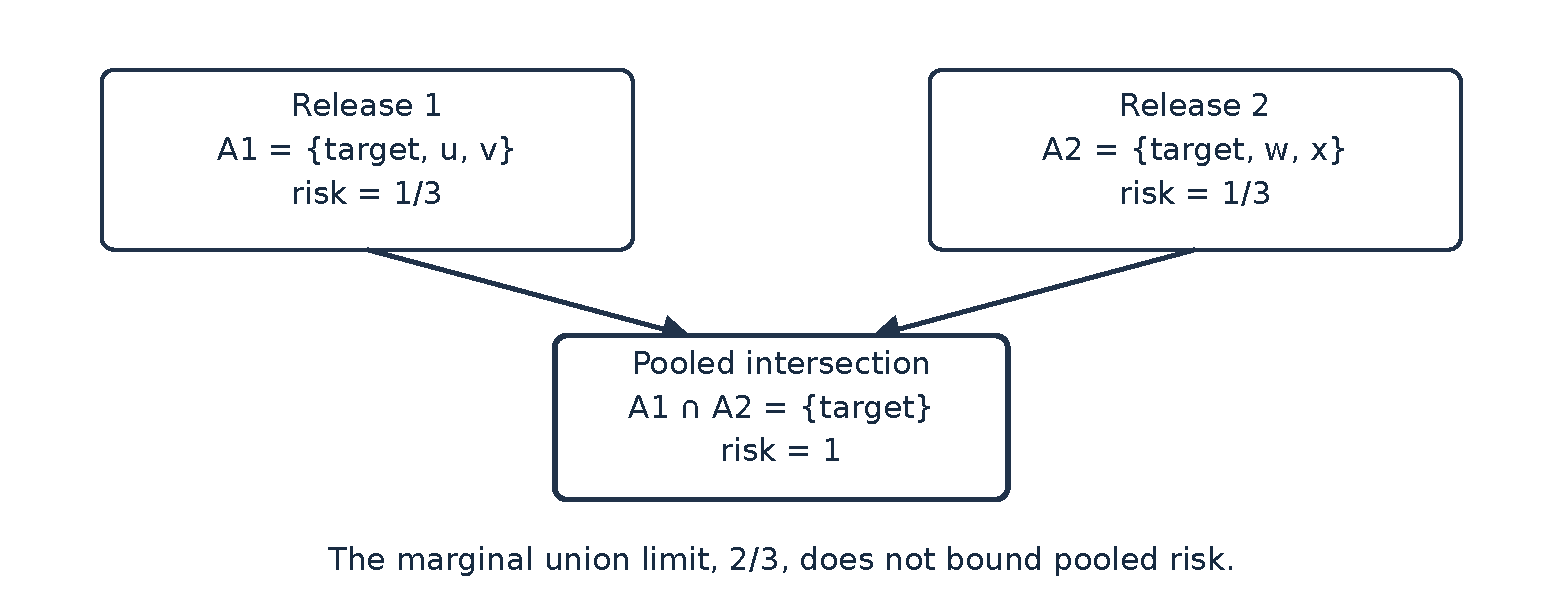
\includegraphics[width=.94\linewidth]{diagrams/pooling.pdf}
\caption{Pooling intersects candidate sets. This illustrative construction assumes uniform selection within each displayed set; it is distinct from the measured four-release simulation.}
\label{fig:pool-diagram}
\end{figure}


The larger difficulty is that $C_\cup$ is the wrong event. An adversary who holds
all $m$ releases is not restricted to using them one at a time. It applies a
joint linkage rule
\begin{equation}
\delta_a^{(m)} : \mathcal{Z} \times \mathcal{Y}_1 \times \cdots \times
\mathcal{Y}_m \longrightarrow I \cup \{\emptyset\} ,
\label{eq:joint}
\end{equation}
and the programme-level risk is $R_{\mathrm{pool}} = \Prob\{\delta_a^{(m)} =
t\}$, which is not contained in the union $C_\cup$.

\begin{proposition}[Marginal risks do not bound pooled risk]\label{prop:nopool}
Let $m \geq 2$. Suppose each released record carries a pseudonym that is the same
in every release, so that records can be matched across releases, and the adversary
knows the target's full quasi-identifier vector, from which it forms the target's key
in every release. For every $\nu > 0$ there exist a population, a sample and $m$
releases such that $R_i \leq \nu$ for every $i$ while
$R_{\mathrm{pool}} = 1$. Consequently no upper bound on $R_{\mathrm{pool}}$ can
be written as a function of $(R_1, \dots, R_m)$ alone. If each release
publishes the candidate set implied by its key and the adversary selects
uniformly from the intersection of those sets, then $R_{\mathrm{pool}}$ is
nondecreasing in $m$ and satisfies $R_{\mathrm{pool}} \geq \max_i R_i$.
\end{proposition}

\begin{proof}
See Appendix \ref{app:proofs}. The construction takes $n = k^m$ units labelled
by vectors in $\{1, \dots, k\}^m$ and lets release $i$ key on all coordinates
except the $i$th, so that every release is $k$-anonymous while the intersection
of the $m$ candidate sets is a singleton.
\end{proof}

\begin{remark}[A persistent pseudonym makes the programme one release]\label{rem:finer}
If every release carries the same pseudonym, the adversary can join the releases
into one table keyed on the union of their key projections. The pooled attack is
then an attack on one finer release, and Proposition \ref{prop:nopool} says that
the finer key can carry far more risk than any of its projections. That is true,
but it is not a composition theorem, and it points to a remedy beside a higher
floor: rotate the pseudonym between releases, so that linkage has to run through
the published fields. Rotation is a control on linkability. It is not
pseudonymisation in the sense of Article 4(5) of Regulation (EU) 2016/679
\citep{gdpr2016}, which concerns whether data can be attributed to a person
without separately held information; a rotated pseudonym leaves the published
fields as they were. The pseudonym itself should be keyed, for example a keyed
hash (HMAC) of the record identifier under a key held apart from the release
team, so that nobody can recompute it from the identifier. Whether rotation helps
depends on the published fields. On the credit register of Section
\ref{sec:eval} it does not while exposure is published exactly, because the
published key and exposure relink every loan; with exposure rounded to one
significant figure they relink about one loan in ten (Section
\ref{sec:eval-programme}). Many release
types, such as aggregates, payment statistics and supervisory tables, carry no
record pseudonym at all, and for them the proposition applies only through
whatever else links the releases.
\end{remark}

The proposition is an existence result, and it says nothing about how large the
gap is in any given programme. Section \ref{sec:composition} measures it on four
releases built from ordinary demographic keys, each carrying a minimum cell count
of three and containing no unique record at all, under the assumption that the
four share a record identifier. The pooled attack identifies the target with
probability 0.4581 against a Boole upper bound of 0.2530. Two releases are already
enough: the pooled risk at $m = 2$ is 0.4114, against a Boole bound of 0.148 for
those two releases, and it is 1.6 times the bound of all four.

Neither the phenomenon nor its direction is new. Complementary releases that are
each $k$-anonymous can be joined to re-identify \citep{sweeney2002}, linked
tables and differencing are an old problem in disclosure control
\citep[ch.~4]{hundepool2012}, and \citet{ganta2008} showed that
independent releases of overlapping populations, each protected by a syntactic
rule, can be combined into a successful attack, and the failure of syntactic
criteria under composition is the standard argument for a formal accountant
\citep{dwork2006a,dwork2014}. The problem of releases that follow one another
has its own literature: \citet{wang2006} anonymise sequential releases of one
table that publish different attributes, \citet{byun2006} treat a table that
grows by insertion, and \citet{xiao2007} define $m$-invariance for a table republished
as records enter and leave: each record keeps the same set of sensitive values
in every version, so intersecting the versions reveals nothing new about it. \citet{cohen2020} prove the same failure for a
formal version of the legal notion of singling out: more than logarithmically
many exact counts, each safe alone, let an adversary single out a record. What Proposition \ref{prop:nopool} adds is a
statement in the terms institutions use to certify releases. The
composition-attack literature shows that combining releases can break a syntactic rule;
the proposition says that no function of the published marginal risks can bound
the combined risk, so the quantity a release programme is certified against is
not the quantity that governs it. Section \ref{sec:eval} then measures that gap on
a synthetic release system with an operational lever.

Three consequences follow for practice. Marginal risk figures may be published,
but they license no programme-level claim. A programme tolerance must be
assessed by direct joint simulation under \eqref{eq:joint}, with shared targets
and shared auxiliary information; separate simulations of each release cannot
recover cross-release dependence by construction, because they never form the
intersection. And a formal accountant, discussed in Section \ref{sec:dp}, is
the one device that does compose without a dependence assumption.

A programme tolerance can also be split among releases as a risk budget on the
union event. Appendix \ref{app:budget} gives the optimal split (Proposition
\ref{prop:budget}) and shows that it differs from the equal split an institution
applies by default. By Proposition \ref{prop:nopool} such a budget governs the
union event only, not the pooled attack, so it allocates attention across
releases and does not replace joint simulation.

\section{Adaptive attacks and anytime-valid certification}\label{sec:sequential}

The preceding analysis fixes the number of releases and attacks. An operational
adversary does neither: it observes a new vintage, decides whether to acquire more
auxiliary information, and stops when the posterior is sufficiently favourable.
An institution also monitors its simulation and may be tempted to stop when the
bound first passes. Fixed-sample intervals do not generally survive either form
of optional stopping. \citet{wald1945} built tests for data that arrive one
observation at a time, \citet{darling1967} and \citet{lai1976} gave confidence
sequences that hold at every sample size, and \citet{johari2022} show how
repeated looks at an online experiment inflate the error of a fixed-sample
test.

Let $\mathcal F_s=\sigma(Y_1,\ldots,Y_s,Z^{(s)})$ be the information available
after release $s$, including auxiliary information acquired adaptively, and let
$H_t$ be the hypothesis that candidate record $j$ belongs to target $t$. The
posterior odds process is
\begin{equation}
O_s(H_t)=O_0(H_t)\prod_{v=1}^s
\frac{p(Y_v,Z^{(v)}\mid H_t,\mathcal F_{v-1})}
     {p(Y_v,Z^{(v)}\mid H_t^c,\mathcal F_{v-1})}.
\label{eq:sequential-odds}
\end{equation}
The conditional densities in \eqref{eq:sequential-odds} prevent the common error
of multiplying marginal likelihoods from dependent vintages. Revisions, common
records and mechanism randomness shared across releases must remain in the
conditioning history.

An adversary need not use the arbitrary posterior threshold one half. Suppose a
correct allegation produces benefit $h>0$, a false allegation costs $c_f\ge0$,
and making the allegation costs $c_a\ge0$. At posterior match probability $p$,
the expected payoff is $ph-(1-p)c_f-c_a$.

\begin{proposition}[Economically rational attack threshold]
\label{prop:attack-threshold}
Suppose an expected-payoff-maximising adversary acts when acting has
nonnegative expected payoff, and abstains when acting cannot gain at any
posterior. If $c_a\ge h$ it never acts, and we write
$p^\star=+\infty$. If $c_a<h$ it acts if and only if
\begin{equation}
p\ge p^\star:=\frac{c_f+c_a}{h+c_f},
\label{eq:attack-threshold}
\end{equation}
and then $p^\star<1$. The threshold equals one half exactly when $h=c_f+2c_a$.
\end{proposition}

The attack evaluation must therefore report the precision--coverage curve over
$p^\star$, or state the payoff assumptions that select one point. A low average
success rate can coexist with a high-payoff attack that makes few, accurate
allegations.

For institutional monitoring, let $X_b\in\{0,1\}$ be success in simulated attack
$b$, $S_B=\sum_{b\le B}X_b$, and consider a candidate risk $r\in(0,1)$. Mixing
the Bernoulli likelihood ratio against a $\mathrm{Beta}(a,b)$ alternative gives
the e-process
\begin{equation}
E_B(r)=
\frac{\mathrm B(a+S_B,b+B-S_B)}{\mathrm B(a,b)
r^{S_B}(1-r)^{B-S_B}}.
\label{eq:eprocess}
\end{equation}

\begin{proposition}[Anytime-valid risk sequence]\label{prop:anytime}
If the simulated attacks are conditionally Bernoulli with risk $r_0$, then
$\{E_B(r_0),\mathcal F_B\}_{B\ge0}$ is a nonnegative martingale with initial
value one. Consequently
\begin{equation}
\Prob_{r_0}\!\left\{\sup_{B\ge1}E_B(r_0)\ge\alpha^{-1}\right\}\le\alpha.
\label{eq:ville}
\end{equation}
The confidence sequence
\begin{equation}
\mathcal C_B=\{r\in(0,1):E_B(r)<\alpha^{-1}\}
\label{eq:cs}
\end{equation}
therefore contains $r_0$ simultaneously for every monitoring time with
probability at least $1-\alpha$ \citep{ville1939,howard2020,howard2021}. The
betting construction of \citet{waudbysmith2024} gives narrower sequences for
bounded means, and \eqref{eq:eprocess} is an instance of the e-values studied
by \citet{vovk2021} and \citet{grunwald2024}.
\end{proposition}

For a family of $q$ targets, mechanisms or subgroups fixed before any outcome
is seen, replacing $\alpha$ by $\alpha/q$ in \eqref{eq:cs} gives simultaneous
anytime coverage without independence, through the union bound. That is what a
report of every coordinate's bound needs. A release that must pass every
coordinate of a fixed family is an intersection--union test, and each coordinate
may keep level $\alpha$ (Section \ref{sec:gov}). The correction is not
valid when $q$ or the choice of family depends on the outcomes. If hypotheses
are added after inspection, $\alpha$ must be allocated by a spending sequence
registered in advance \citep{foster2008,tian2021}, which is the construction of the
companion article. A hierarchical or max-e-process can recover power only if its
dependence model is declared before the results are observed. Control of the
false discovery rate \citep{benjamini1995} is a weaker guarantee and does not
suit a certificate, which must hold for every release it covers.

Finally, calibration on one attack distribution $P$ does not transport without
a condition on the deployment distribution $Q$. The success indicator $C$ is a
function of the attack experiment, so by the data-processing inequality a
declared neighbourhood $D_{\mathrm{KL}}(Q\|P)\le\rho$ gives
$\mathrm{kl}(R_Q\|R_P)\le\rho$, where
$\mathrm{kl}(q\|p)=q\log(q/p)+(1-q)\log\{(1-q)/(1-p)\}$ is the divergence
between two Bernoulli laws. Hence
\begin{equation}
R_Q\le\max\{r\in[0,1]:\mathrm{kl}(r\|R_P)\le\rho\}.
\label{eq:shift}
\end{equation}
The right side increases with $R_P$, so on the event that the upper bound
$\overline R_P$ covers $R_P$ the bound stays valid with $\overline R_P$ in place
of $R_P$, and that is how the pipeline applies it. Pinsker's inequality gives
the looser special case $R_Q\le\min\{1,R_P+\sqrt{\rho/2}\}$, which is far
weaker near zero. The bound is a sensitivity statement over the law of the
data and the auxiliary information, with the attack algorithm held fixed. It
does not describe every change an institution should fear. A new attack
algorithm run on the same data leaves the law unchanged, so it sits at
divergence zero, while its success can move a long way. And the changes that
matter most are large on this scale: halving the standard deviation of the
adversary's exposure reading, from 0.6 to 0.3, is a divergence of about 0.32
per reading. The pipeline implements \eqref{eq:eprocess}--\eqref{eq:shift}, so
optional stopping is measured here and a declared $\rho$ is turned into a bound,
but the main evidence on shift in this paper is the direct rerun at other
reading precisions in Table \ref{tab:replication}.

Appendix \ref{sec:sequential-evidence} reports what these devices give on the
credit release system of Section \ref{sec:eval}. Twenty looks at a fixed-sample
bound put it below the true risk in 21 per cent of 500 runs, against 0 per cent
for the confidence sequence, at the cost of an interval wider by a ratio of 1.05.
An adversary's threshold set by its payoffs changes what it collects from the
same attack. And the programme floor of Section \ref{sec:eval-programme} can
absorb a divergence of well under $10^{-3}$ before its bound reaches the
tolerance.


\section{Formal privacy is a different regime}\label{sec:dp}

A randomised mechanism $M$ is $(\varepsilon, \delta_{\mathrm{dp}})$-differentially
private if, for all neighbouring datasets $x \sim x'$ and all measurable output
sets $E$,
\begin{equation}
\Prob\{M(x) \in E\} \leq e^{\varepsilon}\,\Prob\{M(x') \in E\}
+ \delta_{\mathrm{dp}} .
\label{eq:dp}
\end{equation}
For mechanisms $M_i$ with parameters $(\varepsilon_i, \delta_{\mathrm{dp},i})$,
basic adaptive composition gives $\varepsilon_{\mathrm{tot}} = \sum_i
\varepsilon_i$ and $\delta_{\mathrm{dp,tot}} = \sum_i \delta_{\mathrm{dp},i}$, and tighter accountants are
available \citep{dwork2010,kairouz2017,bun2016,mironov2017,dong2022}. Even the basic form shows the
structural difference from Section \ref{sec:comp}: the composition holds without
any assumption about the adversary or about dependence between releases.

The parameter $\varepsilon$ bounds the change in output distributions for
neighbouring databases. It is not itself the probability that a person is
correctly linked, but it does bound that probability. Read the guarantee as a
limit on hypothesis tests \citep{wasserman2010,kairouz2017,dong2022}. Let an
attack's success be any event that depends on the release and on the target's
record, and let $\kappa$ be its success probability when the target's record is
replaced by another. For an $(\varepsilon,\delta_{\mathrm{dp}})$-differentially
private release, \eqref{eq:dp} applied to that event gives a success of at most
$e^{\varepsilon}\kappa + \delta_{\mathrm{dp}}$, for every attack at once. A
tolerance $\tau$ is therefore met by all attacks together whenever
$e^{\varepsilon}\kappa + \delta_{\mathrm{dp}} \leq \tau$, with $\kappa$ the
largest baseline success the institution admits. The gate of this paper is for
releases that carry no privacy parameter, which is most of what central banks
publish. A second relation is Bayesian and depends on the prior.

\begin{proposition}[What $\varepsilon$ permits]\label{prop:dpbound}
Let $M$ satisfy \eqref{eq:dp} with $\delta_{\mathrm{dp}} = 0$, and let $H$ be a
hypothesis about a single individual such that the databases $x$ and $x'$ under
$H$ and its negation differ only in that individual's record (the replace-one
neighbouring relation), the rest of the database having the same distribution
under both.
For a Bayesian adversary with prior $\Prob(H) = p$, the posterior after
observing that the release falls in a measurable set $E$ of positive
probability satisfies
\begin{equation}
\Prob(H \mid M \in E) \ \leq \
\frac{e^{\varepsilon} p}{e^{\varepsilon} p + (1 - p)} .
\label{eq:dppost}
\end{equation}
\end{proposition}

\begin{proof}
See Appendix \ref{app:proofs}; the argument is the Bayesian reading of
differential privacy in \citet{kasiviswanathan2014}.
\end{proof}

Inequality \eqref{eq:dppost} shows why $\varepsilon$ alone is not a
tolerance. Take an adversary whose prior that a given record is the target's is
$0.1$, because side information outside the release has narrowed the target to
ten candidates. Against a release that is $\varepsilon$-differentially private,
$\varepsilon = 0.5$ permits a posterior of 0.155, $\varepsilon = 1$ permits 0.232
and $\varepsilon = 2$ permits 0.451. With a prior of $1/3$ the same
$\varepsilon = 1$ permits 0.576. An institution that adopts $\varepsilon = 1$
has not chosen a tolerance of 1; it has chosen a multiplier on whatever prior
the adversary brings, and the tolerance it has implicitly accepted depends on
what the adversary knows before it sees the release.

The two regimes therefore answer different questions and both belong in the
record. Scenario-conditional risk answers what a named adversary would achieve
against this release, which is the question a governance committee, a data
protection authority and an affected person all ask. Formal privacy bounds how
far any adversary's beliefs can differ between the release computed with a
record and the release computed without it. That comparison of two posteriors
\citep{kasiviswanathan2014} needs no assumption about how records depend on one
another; only the prior-to-posterior form of Proposition \ref{prop:dpbound}
needs one, because correlated records carry information about each other
\citep{kifer2011}. The guarantee composes across a programme,
which scenario analysis cannot do because Proposition \ref{prop:nopool} denies
it a composition theorem. \citet{kifer2011} show that
neither can be made assumption-free, and the Pufferfish framework of
\citet{kifer2014} makes the adversary's prior an explicit input, which is the
formal counterpart of a declared scenario. \citet{kairouz2017} and
\citet{balle2020} read the guarantee as a limit on the power of any test between
neighbouring datasets, in the sense of \citet{neyman1933}. The practical arrangement is to run a
formal accountant for the programme budget and a scenario assessment for the
release decision, and to report them separately with their assumptions attached.

The distinction decides which tool an institution should use. The framework of this paper is
adversary-specific: it answers what happens if someone with these resources
attacks this release, and the answer is a probability that can be compared with a
tolerance and audited against a stated attacker. Differential privacy is
adversary-agnostic: it answers how much any observer's beliefs can move because
one person's record was included, whoever that observer is and whatever it knows,
and the answer is not a linkage probability. The first is what a release committee
needs, because a committee must justify a decision about a particular publication
to a particular public. The second is what a programme needs, because it is the
only device that composes without an assumption about how releases relate to one
another. An institution that wants both should hold both. The two meet at the
bound $e^{\varepsilon}\kappa + \delta_{\mathrm{dp}}$: for a differentially private
release it turns the privacy parameter into a ceiling on every declared attack,
and the scenario assessment is then needed only to argue for $\kappa$.

\section{Simulation study}\label{sec:sim}

The results above are statements about any release. This section applies them
to a synthetic register where the population is known, so that every estimate
can be compared with a truth. All quantities come from one program with
fixed seeds; Appendix \ref{app:sim} gives the details.

\subsection{Design}

The population has $N = 200{,}000$ units. Each unit carries a district (40
categories with a skewed size distribution), sex, age in single years from 18
to 87, and an occupation group (12 categories, also skewed). The adversary's
key is the cross-classification of district, sex, five-year age band and
occupation group, giving 13,440 possible cells of which 12,596 are occupied.
1,305 cells are population unique, so 0.65 per cent of the population would be
identifiable from the key alone in a census.

The confidential variable is
\begin{equation}
y_i = 8 + \psi_{d(i)} + \omega_{o(i)} + 0.018\,(\mathrm{age}_i - 50)
+ 0.10\,\mathrm{sex}_i + \epsilon_i , \qquad
\epsilon_i \sim N(0, 0.6^2) ,
\end{equation}
with district and occupation effects drawn once from $N(0, 0.45^2)$ and
$N(0, 0.35^2)$. A Bernoulli sample with $\pi = 0.05$ gives $n = 10{,}035$
records containing 4,679 distinct keys, of which 2,729 are unique, so 27.2 per
cent of the released records are sample unique.

The release supports three declared analyses: the mean of $y$ by district, by
five-year age band, and by occupation. Utility \eqref{eq:util} is the negative
of the average of the three root mean squared errors, each computed at the
finest classification its analysis needs and normalised by the standard
deviation of $y$, plus a penalty of $0.5$ times the share of target categories
the release leaves unreportable. Coarsening the key therefore costs accuracy on the analysis it coarsens, and
suppression costs coverage, so both levers reduce measured utility. The two interact: once
a minimum cell count binds, coarsening also buys back records, so the levers are
substitutes as well as costs, which is why the frontier has to be traced rather
than reasoned out.

The declared adversary observes district and sex without error, the released
age band with probability 0.15 of a one-band error, the occupation group with
probability 0.10 of a wrong group, and a noisy reading $z_t = y_t + N(0,
0.75^2)$ of the confidential variable. It links by maximum posterior under the
same error model that generates the error, which is \eqref{eq:post} with a flat
prior over the records in the target's district and sex. The uncertainty set
$H_a$ in \eqref{eq:rob} contains two adversaries, the declared one and one
whose covariate is twice as precise, each modelling its own information
correctly. The robust risk is the larger, and across all 45 settings of the
grid it is attained by the more capable adversary, whose risk runs from 1 to 76
per cent above the declared one, with a median gap of 40 per cent.

Two target sets are reported, because as Section \ref{sec:gov} insists they are
different controls. The first is a target drawn uniformly from the released
records, whose risk is an average; this is the coordinate used for the frontier
and the mechanism grid. The second is the set of records sitting in the smallest
released cells, whose risk is estimated target by target and summarised by its
maximum; this is the supremum control of \eqref{eq:admiss} and it is the
stricter of the two.

The mechanism family is a grid of 45 settings: age band width in
$\{5, 10, 20\}$ years, occupation groups in $\{12, 6, 3\}$, and minimum cell
count $k_{\min} \in \{1, 3, 5, 10, 20\}$ with records in smaller cells
suppressed. A district record swapping lever
\citep{dalenius1982,fienbergmcintyre2004} was built and
then removed. Swapping reduced the simulated risk, but only against an
adversary that takes the released district at face value, and the declared
scenario gives no reason to assume that. Its apparent protection was a property
of the assumed adversary rather than of the release, which is the failure that
Section \ref{sec:est} warns about, so we dropped the lever rather than report a
risk figure that depends on it.

\subsection{The conventional measures disagree by orders of magnitude}

Table \ref{tab:measures} reports the standard summaries for the unprotected
release. The identity \eqref{eq:marksamp} holds exactly: the mean
sample-frequency risk and $D_I/n$ are the same number, 0.4663. The
population-frequency version is 0.0636, and the unconditional measure
\eqref{eq:markpop}, which carries the inclusion probability of
\eqref{eq:factor}, is 0.0233. The sample-frequency measure is 7.3 times the
population-frequency version and 20 times the unconditional one, and all three
have been published under the same label.

\begin{table}[t]
\centering
\caption{Conventional risk summaries for the unprotected release ($N = 200{,}000$, $\pi = 0.05$, $n = 10{,}035$).}
\label{tab:measures}
\begin{tabular}{llr}
\toprule
Measure & Experiment described & Value \\
\midrule
Prosecutor, mean $1/f_k$ & uniform choice among released candidates & 0.4663 \\
Prosecutor, $\max 1/f_k$ & worst released record & 1.0000 \\
Share of records with $f_k = 1$ & sample uniqueness & 0.2719 \\
Marketer, $D_I/n$ & identity \eqref{eq:marksamp}, same experiment & 0.4663 \\
Plug-in $n^{-1}\sum_i 1/F_{K(i)}$ & population frequencies assumed known & 0.0636 \\
Marketer, unconditional \eqref{eq:markpop} & membership unknown, $\pi$ applied & 0.0233 \\
$\pi$ times the plug-in measure & neither experiment; reported anyway & 0.0032 \\
Uniqueness probability $\rho$, truth & $\Prob(F_k = 1 \mid f_k = 1)$, computed & 0.0227 \\
Uniqueness probability $\rho$, model-based & fitted negative binomial for $F_k$ & 0.0274 \\
Journalist, naive $\pi$ & sampling fraction used as the risk & 0.0500 \\
\bottomrule
\end{tabular}
\end{table}


The uniqueness probability $\rho$, reported in the rows of the table headed
uniqueness probability,
is the one measure that needs a model for an unobservable.
If the population frequency law is negative binomial, binomial thinning leaves
it negative binomial with the same dispersion, so the law is identified from the
sample cell counts, and the fit recovers a mean population cell size of 14.83
against a truth of 14.88, within 1 per cent. The closure property fails its own
check, however: the fitted dispersion rises from 0.33 at $\pi = 0.02$ to 0.51 at
$\pi = 0.2$, where the model says it should not move. That drift is evidence of
misfit, and it belongs in falsification test 2 of Section \ref{sec:falsify}. Figure
\ref{fig:journ} compares the resulting $\rho$ with the truth across sampling
fractions. The model-based estimate is conservative at every sampling
fraction and its relative error lies between 8 and 25 per cent. Using $\pi$ itself in place of
$\rho$ overstates the truth at every sampling fraction, by a factor of 2.20 at $\pi = 0.05$ and 1.64 at $\pi = 0.5$.

\begin{figure}[t]
\centering
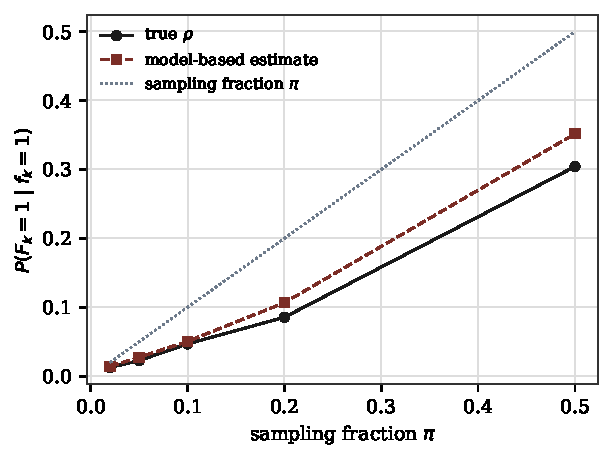
\includegraphics[width=0.62\textwidth]{figures/fig5_journalist.pdf}
\caption{The uniqueness probability $\rho = \Prob(F_k = 1 \mid f_k = 1)$, the
chance that a sample unique is population unique, against the sampling
fraction. The model-based estimate uses a negative binomial population
frequency law fitted to the sample cell counts. The sampling fraction itself is
not an approximation to $\rho$.}
\label{fig:journ}
\end{figure}

\subsection{Measurement error does not simply reduce risk}

Under exact exchangeable matching the predicted success rate for a uniformly
drawn released target is 0.4663. Simulating the declared adversary with key
reporting error but no covariate gives 0.3812 over 5,000 replicates, which is
the reduction practitioners expect. Adding the single noisy covariate returns
the success rate to 0.4642 over 20,000 replicates, with a one-sided 95 per cent
bound of 0.4701. The reciprocal-frequency figure is therefore accurate for this
release, but by cancellation between an error that spreads posterior mass and a
covariate that concentrates it. An assessment that modelled only the reporting
error would have understated the risk by 18 per cent.

Figure \ref{fig:calib} tests the posterior itself, which is the first
falsification requirement of Section \ref{sec:falsify}. When the adversary's
declared model matches the process that generates its information, the mean gap
between the binned maximum posterior and the empirical success rate is 0.007.
When the adversary assumes a covariate 2.5 times noisier than the truth, the mean gap rises to 0.049 and the miscalibration is one-sided: the posterior
understates the success rate in the lower bins. The overall success rate barely
moves, from 0.4642 to 0.4571. This is the practical lesson of the figure.
A single risk number cannot reveal that the linkage model is wrong, and a
calibration check on held-out matches can.

\begin{figure}[t]
\centering
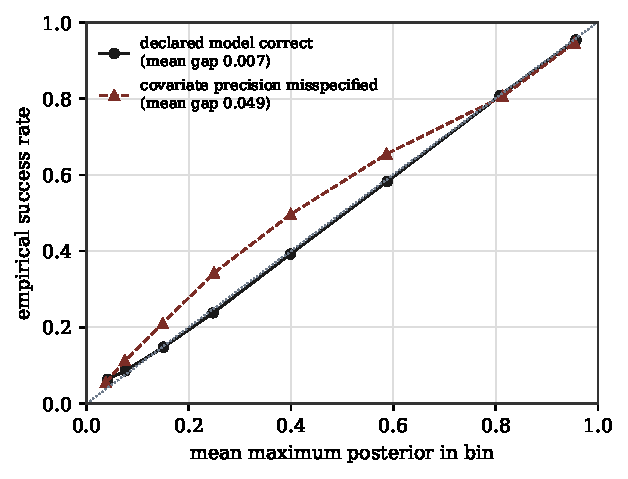
\includegraphics[width=0.58\textwidth]{figures/fig3_calibration.pdf}
\caption{Calibration of the adversary's maximum posterior against the empirical
success rate, 20,000 replicates per curve. The two models produce risk estimates
that differ by 0.007, while their calibration gaps differ by a factor of seven.}
\label{fig:calib}
\end{figure}

\subsection{$k$-anonymity does not deliver $1/k$}\label{sec:kanon}

Table \ref{tab:kanon} applies minimum cell counts and compares the nominal
bound $1/k$ with two simulated quantities: the average risk over a uniformly
drawn released target, and the risk of the worst target among those in the
smallest released cells, each of the latter estimated from 250 replicates.

The average risk stays below $1/k$ at $k = 3$ and $k = 5$ and exceeds it at
$k = 10$ and $k = 20$. The worst target's risk exceeds $1/k$ at every $k$, and so does its one-sided
95 per cent lower confidence bound, which is 0.82, 0.78, 0.64 and 0.68 as $k$
runs from 3 to 20. Those bounds carry a Bonferroni correction for the number of
targets examined, since the worst target is selected on its own estimate.
Between 27 and 75 per cent of the targets in minimum-size cells have an
individual lower bound above $1/k$. Both comparisons show that $k$-anonymity on
the declared key does not deliver $1/k$ when the intruder also holds a reading
of the released continuous variable, and the second shows it in the form that
matters for rule \eqref{eq:admiss}, which is stated as a supremum. This is a
failure of key selection, not of the criterion: the covariate separates members
of a key class, and raising $k$ on a key that leaves it out shrinks the share of
the adversary's information that the criterion controls while leaving the
covariate untouched.

Figure \ref{fig:riskdist} shows what the suppression does to the whole risk
distribution rather than to its maximum, and the utility loss is large. Reaching
$k = 10$ retains 15.5 per cent of the released records and reaching $k = 20$
retains 4.8 per cent, so a release governed by its maximum prosecutor risk
alone is pushed towards discarding most of its own content.

\begin{table}[t]
\centering
\caption{Minimum cell counts against the simulated risk of the declared adversary. The average uses 12{,}000 uniformly drawn targets with $\overline{R}_{0.95}$ its one-sided Clopper--Pearson bound. The worst target is taken over the listed number of targets in minimum-size cells, each estimated from 250 replicates, and is reported with a one-sided 95 per cent lower bound carrying a Bonferroni correction for the number of targets examined. The last column is the share of those targets whose individual lower bound exceeds $1/k$.}
\label{tab:kanon}
\small
\begin{tabular}{rrrrrrrrr}
\toprule
$k_{\min}$ & Kept & Share & $1/k$ & Average & $\overline{R}_{0.95}$ &
Targets & Worst (bound) & Share above $1/k$ \\
\midrule
3 & 5{,}426 & 0.541 & 0.3333 & 0.2573 & 0.2640 & 250 & 0.900 (0.817) & 0.748 \\
5 & 3{,}361 & 0.335 & 0.2000 & 0.1852 & 0.1911 & 250 & 0.868 (0.778) & 0.492 \\
10 & 1{,}555 & 0.155 & 0.1000 & 0.1129 & 0.1178 & 230 & 0.744 (0.638) & 0.326 \\
20 & 484 & 0.048 & 0.0500 & 0.0787 & 0.0828 & 60 & 0.768 (0.675) & 0.267 \\
\bottomrule
\end{tabular}
\end{table}


\begin{figure}[t]
\centering
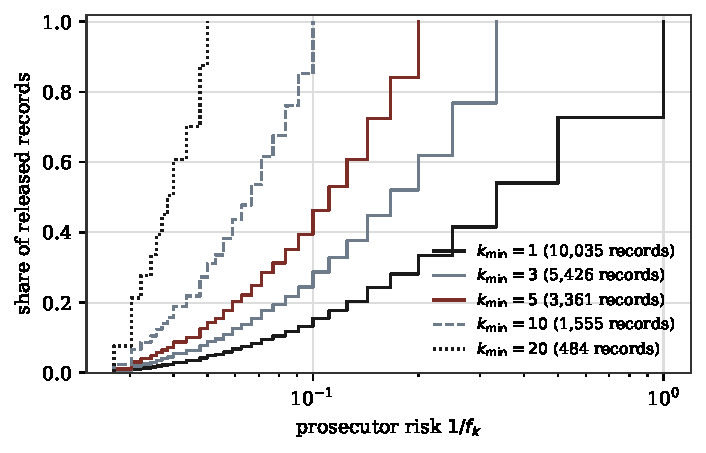
\includegraphics[width=0.66\textwidth]{figures/fig1_risk_distribution.pdf}
\caption{Distribution of prosecutor risk $1/f_k$ across released records under
minimum cell counts. Governing the maximum alone forces most of the file out of
the release.}
\label{fig:riskdist}
\end{figure}

\subsection{Frontier, tolerance and the relative weight assigned to harm}

Figure \ref{fig:frontier} plots all 45 mechanism settings in the plane of the
one-sided risk bound and the utility of Section \ref{sec:ru}. Eleven settings
are nondominated, and the frontier spans risk from 0.081 to 0.564. It is steep
at the low-risk end: halving the bound from 0.1715 to 0.0806 costs 0.17 of
utility, half the range the frontier spans, and cuts the records retained from
100 to 58 per cent.

The attainable frontier is not concave. Successive slopes of the eleven
nondominated points run from 6.0 down to 0.006 and not monotonically,
which is what a discrete mechanism family produces and what Proposition
\ref{prop:exist} anticipates. A three-parameter power curve fits it with $R^2 = 0.964$ and is concave over the
fitted range; it is used only for the allocation
in Section \ref{sec:composition}, which is therefore a stylised illustration on
a fitted curve, not an optimum over the discrete settings. Table \ref{tab:tau} reports the implied
tolerance of Proposition \ref{prop:tau}, computed as the value-maximising choice
over the eleven nondominated settings rather than on the fitted curve, and with
the one-sided bound as the risk coordinate as \eqref{eq:admiss} requires.

Two features matter for practice. The implied tolerance is flat over wide
ranges, since one setting is optimal from $\kappa = 5$ to $\kappa = 10$, and it
jumps between ranges: doubling the relative weight assigned to harm from $\kappa = 0.5$ to $\kappa = 1$ cuts the tolerance
from 0.345 to 0.145 and moves the release from an unsuppressed file with twelve
occupation groups to one with three groups and a minimum cell count of five. The jump is a property of the discrete mechanism
family, not of the argument, and it has a practical reading: over most of the
range an institution cannot fine-tune its tolerance, and near a breakpoint a
small revision of the relative weight assigned to harm changes the release.

\begin{figure}[t]
\centering
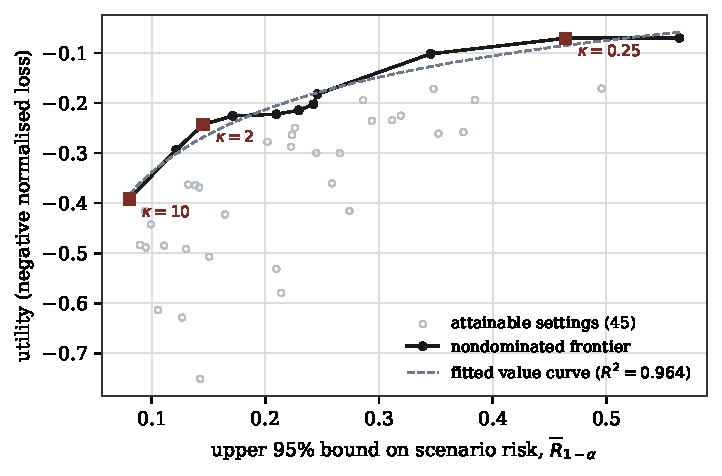
\includegraphics[width=0.72\textwidth]{figures/fig2_frontier.pdf}
\caption{Risk--utility plane for 45 mechanism settings. The risk coordinate is
the one-sided 95 per cent bound for a uniformly drawn target, not the point
estimate. Squares mark the value-maximising setting for three values of the
relative harm weight $\kappa$; the associated risk is the implied
tolerance $\tau^\star$ of Proposition \ref{prop:tau}.}
\label{fig:frontier}
\end{figure}

\begin{table}[t]
\centering
\caption{Tolerance implied by the relative harm weight, computed by maximising $U - \kappa \overline{R}_{0.95}$ over the nondominated settings. The selected setting reports age band width in years, occupation groups and minimum cell count.}
\label{tab:tau}
\begin{tabular}{rrlr}
\toprule
$\kappa = c_h/\lambda$ & Implied $\tau^\star$ & Selected setting & Records kept \\
\midrule
0.25 & 0.464 & 10-year bands, 12 groups, $k_{\min} = 1$ & 1.00 \\
0.50 & 0.345 & 20-year bands, 12 groups, $k_{\min} = 1$ & 1.00 \\
1.00 & 0.145 & 20-year bands, 3 groups, $k_{\min} = 5$ & 0.94 \\
2.00 & 0.145 & 20-year bands, 3 groups, $k_{\min} = 5$ & 0.94 \\
5.00 & 0.081 & 20-year bands, 3 groups, $k_{\min} = 20$ & 0.58 \\
10.00 & 0.081 & 20-year bands, 3 groups, $k_{\min} = 20$ & 0.58 \\
\bottomrule
\end{tabular}
\end{table}


\subsection{A programme of four releases}\label{sec:composition}

Four releases are built from the same sample. Release A keys on district, sex
and five-year age band; release B on district, sex and occupation; release C on
district, ten-year age band and six occupation groups; release D on sex,
ten-year age band and occupation. Each applies a minimum cell count of three,
so each is 3-anonymous and, by construction, no release contains a single
unique record. Their marginal risks, computed unconditionally so that a target suppressed from
a release contributes zero, are 0.0768, 0.0711, 0.0884 and 0.0168.

The pooled adversary below assumes that the four releases carry a common record
identifier, so that it can intersect the target's candidate sets across them.
Four releases cut from one sample need not carry one, and without it the
adversary would have to link records through the published keys; we did not
measure that case here. With a common identifier the four releases are one
release keyed on the union of their keys (Remark \ref{rem:finer}), and the
figures below measure how much finer that union is than any of its parts.

Table \ref{tab:comp} and Figure \ref{fig:comp} report what the programme
permits. The bounds implied by the marginals are $[0.0884, 0.2530]$ and the
independence value is 0.2313. An adversary that intersects the candidate sets of
the first two releases succeeds with probability 0.4114, which is 2.8 times the
bound of 0.148 implied by those two marginals and 1.6 times the upper bound implied
by all four. With all four releases the pooled risk
is 0.4581, which is 1.8 times that bound, and 26.0 per cent of targets are
uniquely identified by the intersection although none was unique in any single
release.

\begingroup\small\setlength{\tabcolsep}{3pt}\begin{table}[t]
\centering
\caption{Four 3-anonymous releases from one sample, 20{,}000 target replicates. No single release contains a unique record. Marginal risks are unconditional; a target suppressed from a release contributes zero to that release and does not narrow the intersection. The pooled adversary intersects the candidate sets of releases 1 to $m$ and selects uniformly from the intersection.}
\label{tab:comp}
\begin{tabular}{lrrr}
\toprule
& Records released & Marginal risk & Unique share \\
\midrule
Release A (district, sex, fine age) & 9{,}648 & 0.0768 & 0.000 \\
Release B (district, sex, occupation) & 9{,}709 & 0.0711 & 0.000 \\
Release C (district, ten-year age, six groups) & 9{,}257 & 0.0884 & 0.000 \\
Release D (sex, ten-year age, occupation) & 10{,}035 & 0.0168 & 0.000 \\
\midrule
\multicolumn{4}{l}{\emph{Programme-level quantities}} \\
Lower bound $\max_i R_i$ & & 0.0884 & \\
Upper bound $\min(1, \sum_i R_i)$ & & 0.2530 & \\
Value under independence & & 0.2313 & \\
Pooled attack, $m = 2$ & & 0.4114 & 0.208 \\
Pooled attack, $m = 3$ & & 0.4279 & 0.222 \\
Pooled attack, $m = 4$ & & 0.4581 & 0.260 \\
\bottomrule
\end{tabular}
\end{table}
\endgroup

\begin{figure}[t]
\centering
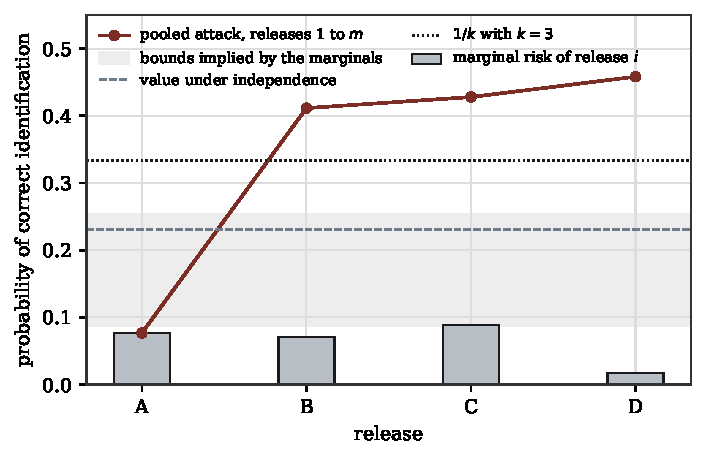
\includegraphics[width=0.72\textwidth]{figures/fig4_composition.pdf}
\caption{Marginal risks of four 3-anonymous releases and the risk of an
adversary that pools them. The shaded band is the interval implied by the
marginals under Proposition \ref{prop:boole}. The pooled attack leaves the band
at $m = 2$.}
\label{fig:comp}
\end{figure}

Two remarks. First, the effect is not driven by a large number of releases. Two
are enough, and the third and fourth add little because the first two already
carry most of the separating information. Second, on this draw, ranking
releases by their own risk figures does not rank their contribution to the
programme: release D has the smallest marginal risk, 0.0168, yet adding it to the
pool raises the risk by 0.030, while release C, whose marginal risk is the
largest at 0.0884, adds 0.017. The contributions depend on the order in which
releases are added and rest on one sample, so we read this as an example that
the two rankings can differ, not as a finding about releases C and D.
Neither observation is visible in a marginal assessment.

Applying Proposition \ref{prop:budget} to the union event, with value weights
$1, 0.7, 0.5, 0.3$ and $\tau_{\mathrm{prog}} = 0.50$, the optimal allocation is
$(0.186, 0.139, 0.106, 0.070)$ against the equal split of $0.125$ each, and cuts
the total loss by 4.5 per cent on the fitted curve. A constrained numerical
optimum agrees with the closed form \eqref{eq:power} to five decimal places, which
is one check on both. With the fitted $\gamma = -0.23$ the exponent in
\eqref{eq:power} is 0.81, so the allocation is flatter than the value weights.
This is a stylised illustration on a fitted curve, not an optimum over the
discrete settings, whose frontier is not concave; the gain is small, and it is
available only for the union event.

\subsection{Further checks}

Appendix \ref{app:further} reports three further checks on the synthetic
population: whether the gap between pooled and marginal risk survives at other
register sizes (it widens, Table \ref{tab:scaling}), what certifying a small
tolerance costs in simulated attacks (Table \ref{tab:cert}), and how much of the
variance of a risk estimate the binomial interval misses (Section
\ref{sec:nested}).

\subsection{Reproducing the study}\label{sec:repro}

Everything above comes from one program with a single seed, packaged in the
companion repository. The package keeps four kinds of work apart and labels
them: proof checks that verify algebraic consequences of the declared
assumptions, simulation checks that estimate attack success and its Monte Carlo
error, falsification tests that can reject the model, and the governance gate
that applies the tolerance. A run writes the configuration it used, every
result, the validation status, the five figures, the LaTeX fragments for the
tables in this section, a decision record naming the tolerance, owner, expiry
date and adversary, and a SHA-256 hash of each of those files. A failed
falsification test produces a non-zero exit status, so a rejected model cannot
be presented as governed evidence.

Two details of that arrangement matter for a reader checking this paper. The
tables in this section are generated by the run rather than typed, so a table
cannot disagree with the experiment that produced it. And the figures quoted in
the prose are checked against the run by a script that fails when one of them
drifts. The script checks every value the run writes to its number file and every
quoted decimal with three or more places; integers and two-place figures are
checked by hand. The run reported here selects the 20-anonymous setting under a
tolerance of 0.12. Its single-release upper bound meets the tolerance, so the
release check passes, but the upper bound on the pooled risk of the declared
four-release programme, 0.464, exceeds the release tolerance, and the gate
therefore returns a fail. The programme check compares the upper bound, not the
point estimate of 0.4581, with the tolerance, for the reason of Proposition
\ref{prop:point}. The programme validation check uses its own tolerance of 0.50,
which is recorded separately and plays no part in that decision. A failed
decision is the intended outcome here: the gate fails closed when the programme
is riskier than the tolerance the release was set. The credit evaluation of Section \ref{sec:eval}
was also rerun over 20 independent register draws by a separate script,
\texttt{scripts/programme\_robustness.py} (Table \ref{tab:replication}).

\section{Real data}\label{sec:real}

Everything above is measured on data we generated, which is the only way to check
an estimator against a truth. It is not a substitute for running the framework on
a file someone actually published. This section does that, on two real public
microdata files that ship with the \texttt{wooldridge} package: an extract of the
US Census 2000 public use sample, 29,501 records with state, public use microdata
area, years of schooling, potential experience and log weekly income; and the
Boston Fed mortgage application study, 1,986 real applications with area, income,
marital status, dependants, occupancy, the lending decision and a record of late
payments. Both files are already public and already protected. Nothing
confidential is read here, and the question asked is the one an agency asks before
publishing a file of that shape: what would a declared adversary achieve against
it.

Three things change when the data are real, and each of them is a claim the
earlier sections make. The population behind the file is not observed, so the
population-frequency measure cannot be computed at all and the uniqueness
probability $\rho$ has no truth to be checked against: a fitted model is the only route to it, which
is why Section \ref{sec:falsify} asks for a frequency-transport test rather than a
comparison. The analyses that define utility are given by what the file is used
for, not chosen by us. And the risk levels are much higher than in the simulation,
so the choice of tolerance matters more.

\subsection{The census sample}

The figures in this subsection are a demonstration that the pipeline runs on a
real published file. They are prosecutor risks computed inside the file, for an
adversary who knows that its target is in the extract. They are not an estimate
of the risk the file posed to the population, which a statistical office would
assess with the sampling fraction, the population frequencies and the access
conditions that we do not have.

On the full key, state, area, schooling and experience, the 29,501 records occupy
27,390 classes. Of those classes 92.9 per cent are unique, and they hold 86.3 per
cent of the records. The mean reciprocal frequency
is 0.928. This is a published file, so the finding is not that someone blundered:
it is that the key an outsider can reconstruct almost determines the record, and
that any protection claim about it has to come from something other than the key.
The key space, counting the areas actually observed inside each state, holds
665,896 cells. The uniqueness probability $\rho$ needs the file's sampling fraction, which
is not known, and the pipeline assumes $\pi = 0.05$. Under that assumption a
negative binomial law fitted to the observed counts puts the mean population
cell at 0.886 people once empty cells are counted, and a record unique in the
file is unique in the population with probability 0.225. The figure is a
consequence of the assumed $\pi$, not a finding about the file. With the
dispersion held at its fitted value, $\rho$ is 0.035 at $\pi = 0.01$ and falls further at smaller fractions, and the
file, a small subsample of the 2000 public use sample, covers a fraction of the
US population far below 0.05. There is no truth here to compare these with, which is the position an
agency is in when it does not know its own sampling fraction.

Table \ref{tab:real} reports the releases on the frontier of 25 settings that vary
the area, schooling and experience bands and the minimum cell count. The declared
adversary observes the key exactly but models a misreading probability of 0.10,
and holds a noisy reading of income. The column headed Simulated is the robust
risk, the larger of the risks of this adversary and one whose income reading is
twice as precise. The simulated attack beats exact matching at every setting, by
a factor between 1.05 and 4.19: at the widest bands with a minimum cell count of
ten, exact matching gives 0.062 and the simulated attack gives 0.239.

Utility charges for coarsening as well as for suppression. Each of the three
analyses is estimated at the fine level of its variable, and a release that
publishes a band supplies the band mean for every fine level inside it, as in
Section \ref{sec:sim}; so a release with four-year schooling bands loses accuracy
on income by schooling even when it suppresses nothing. The frontier then holds
eight of the 25 settings, and it runs from 0.276 to 0.942 under simultaneous
one-sided bounds over the 72 planned setting--adversary comparisons. These are
conditional attack success rates against the tested public file, not population
re-identification rates or certificates against untested attacks. The
pipeline also reads implied tolerances off this frontier, as in Section
\ref{sec:sim}; we do not report them, because a tolerance for a file of this kind
is a policy choice for the office that publishes it, and in-file prosecutor risks
are not the quantity it would govern. The settings with the finest bands sit at
the high-risk end of the frontier, where they buy the last units of utility.

\begin{table}[t]
\centering
\caption{US Census 2000 public use sample: the nondominated releases. The file holds 29{,}501 records, and the columns report the width of the area, schooling and experience bands, the minimum cell count, the share of records kept, the risk under exact matching, the simulated risk with its simultaneous one-sided bound over the 72 planned setting--adversary comparisons, and the utility across the three income analyses. The simulated risk is the larger of two adversaries, the declared one and one with a covariate reading twice as precise. Both read the key exactly but model a misreading probability of 0.10, and both hold a noisy reading of log weekly income.}
\label{tab:real}
\small
\begin{tabular}{rrrrrrrrr}
\toprule
Area & Schooling & Experience & $k_{\min}$ & Kept & Exact matching & Simulated & $\overline{R}_{0.95}$ & Utility \\
\midrule
100 & 4 & 10 & 10 & 0.284 & 0.0615 & 0.2393 & 0.2761 & -0.330 \\
10 & 4 & 10 & 10 & 0.253 & 0.0680 & 0.2713 & 0.3094 & -0.327 \\
100 & 4 & 10 & 5 & 0.566 & 0.1093 & 0.3407 & 0.3808 & -0.161 \\
10 & 4 & 10 & 5 & 0.554 & 0.1165 & 0.3567 & 0.3972 & -0.155 \\
100 & 4 & 10 & 1 & 1.000 & 0.2965 & 0.5060 & 0.5475 & -0.097 \\
100 & 1 & 10 & 1 & 1.000 & 0.4282 & 0.6567 & 0.6954 & -0.071 \\
100 & 4 & 1 & 1 & 1.000 & 0.7418 & 0.8827 & 0.9077 & -0.026 \\
100 & 1 & 1 & 1 & 1.000 & 0.8348 & 0.9213 & 0.9419 & -0.000 \\
\bottomrule
\end{tabular}
\end{table}


\paragraph{Selection and uncertainty.} Figure \ref{fig:real-audit} lays out the
public-file evaluation in the order it runs: the public files, the declared
releases, the attack simulation on fresh targets, the 72 exact bounds that share
one familywise error of 0.05, the frontier chosen from them, and the sensitivity
checks, which sit outside that family. The frontier is chosen after the bounds
are computed, and the familywise bound is what keeps that choice valid. The
grid plans $3\times2\times2\times3=36$
settings and two attacker precisions, although only 25 settings retain at least
500 records. For planned pair $j\in\{1,\ldots,72\}$ let $K_j$ be its number of
successful attacks in $n_j=1500$ independently sampled targets, with fresh
auxiliary noise, conditional on the released file and fixed attack rule. If
$U_j=B^{-1}_{1-\alpha/72}(K_j+1,n_j-K_j)$ for $K_j<n_j$, and $U_j=1$
otherwise, where $B^{-1}_q(a,b)$ is a beta quantile, then
\[
 \Pr\{\forall j:\ p_j\le U_j\mid\text{these public files}\}\ge1-\alpha,
 \qquad \alpha=0.05.
\]
This follows from the exact one-sided binomial bound and a union bound; it does
not assume independence between settings. Each setting's reported upper risk
is the maximum of its two $U_j$ values. Hence selecting a frontier setting
after viewing all simulated attacks does not undo this familywise Monte Carlo
coverage. The result does not cover a new attacker, a new file, uncertainty in
the source population, or adaptive additional grid searches. The utility is
measured against analyses of the public extract itself, rather than population
ground truth.

\begin{figure}[H]
\centering
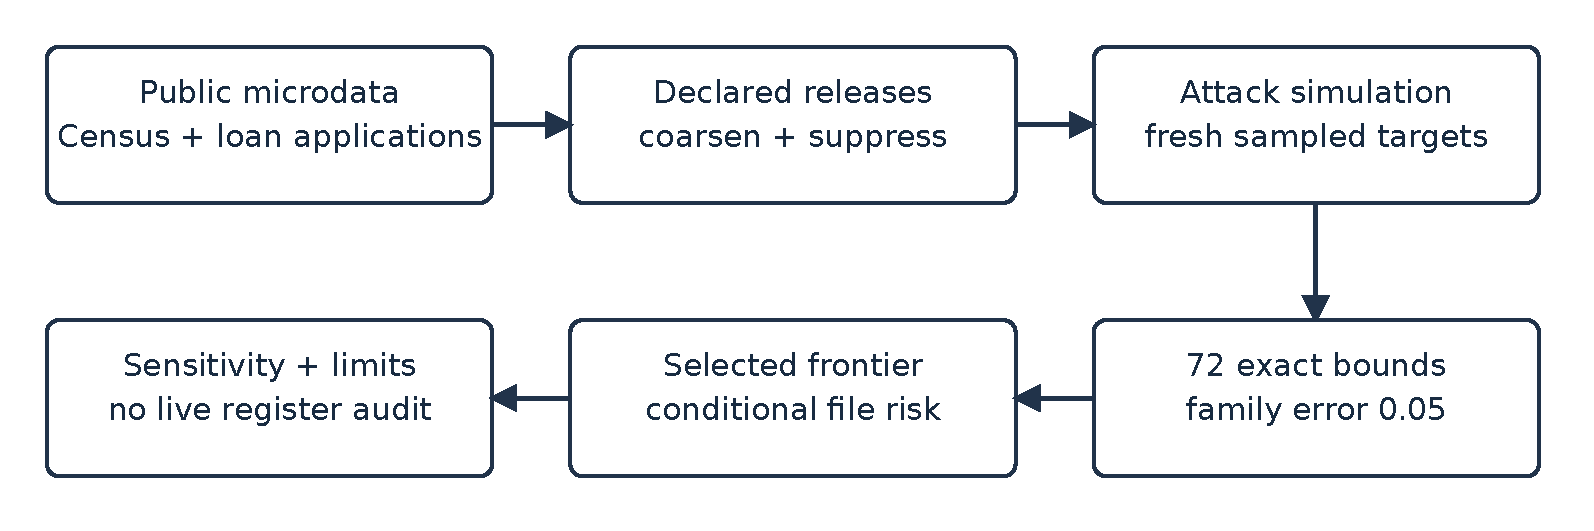
\includegraphics[width=.96\linewidth]{diagrams/realdata_audit.pdf}
\caption{Public-file evaluation. The familywise bound covers the planned
36 release settings and two attacker precisions on the census file,
conditional on the released file and independent sampled targets. Sensitivity checks are
exploratory; a separate audit is needed for a live register.}
\label{fig:real-audit}
\end{figure}


The attacker assumption matters: on one setting of the grid, a separate
exploratory run with 3,000 targets, archived in
\texttt{artifacts-real/replication.json}, gives success rates 0.371, 0.271 and 0.186
as the standard deviation of its log-income reading changes from 0.25 to 0.5
to 1.0. On the loan file the corresponding rates are 0.179, 0.137 and 0.093
for loan-amount standard deviations 20, 40 and 80. These additional rates have
individual 95 per cent intervals only and do not extend the 72-comparison
family. They make the assumed quality of auxiliary information visible rather
than treating one risk value as intrinsic to the file.

The supremum control needs a setting to act on, and the run takes the middle
setting of the frontier, which has four-year schooling bands and no minimum cell
count. The 80 records it examines sit in classes of 1. The attack names them with
mean probability 1.000, and the worst of them is identified with probability 1.00,
with a Bonferroni-corrected lower bound of 0.964. On this setting the key alone
separates them, so the check shows how exposed an unsuppressed release of this
file is; it does not test a $k$-anonymity promise, because the setting makes
none, and we do not compare it with the simulated register of Section
\ref{sec:kanon}.

Composition was run on this file under the same condition as Section
\ref{sec:composition}: the four releases are taken to share a record identifier,
so that a record can be matched across them. Four public-use files cut from one
census sample would not carry common record identifiers, and an adversary would
then have to link them through the published fields; we did not measure that case
on the census file. With the shared identifier, four releases were built by
dropping one key component at a time, each with a minimum cell count of three.
Their marginal risks are 0.138, 0.030, 0.118 and 0.096, so the union bound is
0.381. The pooled adversary reaches 0.709, which is 1.86 times that bound, and
60.7 per cent of targets are uniquely identified by the intersection although none
of the four releases contains a unique record. On the synthetic register the same
comparison gave 1.8 times the bound. Each figure comes from one draw, so the two
do not show that the effect is larger on either kind of data.

\subsection{The mortgage applications}

The second file, the Boston Fed mortgage applications, is small and shows the
other risks of Section \ref{sec:credit}: identification against a noisy reading
of the loan amount, attribute disclosure of the lending decision and of late
payments, and residual disclosure from published totals. Appendix
\ref{app:mortgage} reports the figures. Unlike the synthetic credit register,
both harmful directions of attribute disclosure occur in it.

\subsection{What the real files settle and what they do not}

Two findings from the generated data reappear on the two public files: the
covariate beats exact matching at every setting, and, when the releases share a
record identifier, the pooled attack exceeds the marginal bound.

Four limits should be read with the numbers. The files are samples whose
populations are not observed, so the uniqueness probability $\rho$ rests on an assumed
sampling fraction and a fitted law that this exercise cannot check, and the utility analyses are computed against the file
rather than against the population it came from. The adversary is declared, not
observed: the reporting error rate and the precision of the income reading are
assumptions, and Section \ref{sec:falsify} is how an institution would test them.
And these are public files, so the exercise measures what a release of this shape
discloses, not whether a wrong was done in publishing them. And only the
demographic path of the pipeline ran on these files: the credit evaluation of
Section \ref{sec:eval} has run only on the synthetic register.

\section{A granular credit register}\label{sec:credit}

Many central banks collect loan-level credit data under statute. In the euro
area, AnaCredit collects, mostly monthly, data on loans by credit institutions to
legal entities, not households, whenever the debtor's commitment amount with the
reporting institution is at least EUR 25{,}000, and each record ties a borrower to
a lender \citep{ecb2022}. The Irving Fisher Committee has discussed the use of
such micro data across jurisdictions \citep{ifc2016}, and \citet{israel2017}
describe the content and uses of AnaCredit. Loan-level registers also support
research on credit supply: \citet{khwaja2008} use a credit register to separate
supply from demand, and \citet{jimenez2012} use loan applications in the Spanish
register to identify the bank balance-sheet channel. Loan-level data of this
kind are not released for general use; research access is restricted. The
releases studied here are therefore a stylised set of three kinds: a loan-level
file of the sort a secure research environment might give access to, aggregates
by region, sector and lender, and a monthly series with revisions. The borrowers
are firms. That combination is what makes a credit register a different problem
from a demographic file, and it is the problem this section measures on a
synthetic register built to share the structure of a supervisory collection.

Five harms have to be told apart, because a single risk figure covers only one of
them. A borrower may be identified. A borrower--lender relationship may be
alleged, whether or not the borrower is identified. Arrears, default or
forbearance status may be inferred for a class of borrowers without identifying
anyone. One lender's contribution may be reconstructed from published totals by
another participant. And two consecutive vintages may be differenced. Table
\ref{tab:credit} reports all five against one lever, a minimum cell count on the
borrower key.

The simulated register has 20{,}000 borrowers, 60 lenders, 18 sectors, 12
regions and 4 size classes, so the borrower key has 864 cells. It runs for six
monthly vintages. Most loans are outstanding when the panel opens and the rest
are originated in a later month; every loan then leaves with a monthly hazard of
0.04 and does not come back. The stock stays near 27{,}000 loans, about 4 per
cent of it turns over each month, and 81 per cent of the loans in the first
release are live in all six. Over the six months 32{,}581 loans are observed,
and the first release holds 27{,}167 of them. Exposure is lognormal within size
class and arrears occur at 7 per cent. Appendix \ref{app:sim} gives the details.
The lenders hold unequal shares, the largest 23 per cent. One simplification
matters for everything that follows: a loan's exposure is the same in every
vintage in which it is live. A real register reports outstanding amounts that
change as loans are drawn and repaid, and we have not modelled that.

\begin{table}[t]
\centering
\caption{Credit register: five risks and one utility under a minimum cell count on the borrower key. The register holds 32{,}581 relationships between 20{,}000 borrowers and 60 lenders. Identification is the average over released relationships with its one-sided bound, and again for the largest size class alone. The predictive value is that of an alleged borrower-lender relationship, and the homogeneity share is the proportion of large borrowers whose key class discloses their arrears status. Utility is the negative weighted loss across credit growth, concentration, the arrears ratio and lender-level supervision.}
\label{tab:credit}
\small
\begin{tabular}{rrrrrrrr}
\toprule
$k_{\min}$ & Kept & Identification & $\overline{R}_{0.95}$ & Large firms & Relationship PPV & Status disclosed & Utility \\
\midrule
1 & 1.000 & 0.0855 & 0.0931 & 0.247 & 0.328 & 0.444 & -0.000 \\
5 & 0.990 & 0.0770 & 0.0843 & 0.273 & 0.324 & 0.381 & -0.050 \\
10 & 0.958 & 0.0705 & 0.0775 & 0.119 & 0.320 & 0.262 & -0.139 \\
20 & 0.851 & 0.0563 & 0.0626 & 0.155 & 0.313 & 0.119 & -0.254 \\
\bottomrule
\end{tabular}
\end{table}


\paragraph{Identification is a subgroup problem.} Success can be scored two ways,
and the difference matters. Recovering the exact relationship succeeds for 0.0855
of released rows, with a one-sided bound of 0.0931; recovering the right borrower,
which is the harm the register creates, succeeds for 0.1095, because a borrower
with several lenders can be found through any of them. Both look comfortable as
averages. Split by size class the relationship figure is 0.050, 0.091, 0.128 and
0.247, so a large borrower faces about five times the risk of a micro borrower.
This is the target-set point of Section \ref{sec:gov}: the same file meets any
tolerance its average figure meets and breaches that tolerance on the largest
size class. Raising the minimum cell count to 20 brings the large-borrower
figure to 0.155 and keeps 85 per cent of the relationships. That subgroup rests
on few targets, so it is reported with its interval: [0.192, 0.309] at
$k_{\min} = 1$ and [0.085, 0.250] at $k_{\min} = 20$. The two overlap, and the
risk is not monotone across the grid: it is 0.273 at $k_{\min} = 5$ and 0.119 at
$k_{\min} = 10$. The large-firm figure at no suppression agrees across draws: it
is 0.248 in Table \ref{tab:eval}, which scores the same event on its own draw,
and about 0.24 on a stratified draw of 4{,}000 large-firm targets (Section
\ref{sec:eval-programme}). A uniform draw holds only a few hundred large-firm
targets, which is why the subgroup floor of Section \ref{sec:eval-programme} uses
the stratified draw.

\paragraph{An alleged relationship is a base-rate statement.} Suppose the
adversary names, for every borrower in the release, the lender holding the
largest share of that borrower's key class. Equation \eqref{eq:ppv} gives the
quantity that matters, the probability that an allegation is true. On the
simulated register the prevalence of any given borrower--lender pair is 0.0243,
the sensitivity of this rule is 0.225 and its specificity is 0.989, and
\eqref{eq:ppv} returns 0.328, which is the realised share of correct
allegations. The four cells are reported so that a reader can check the identity
rather than take the predictive value on trust; their agreement is arithmetic,
not evidence. Two readings follow. A specificity of 0.989 sounds protective and
is not, because the prevalence is low. And an allegation that is right a third
of the time is 1.4 times the success rate of always naming the largest lender in
the market (share 0.23), and wrong about two borrowers in three. The minimum cell
count barely moves it: 0.328 at $k_{\min} = 1$ and 0.313 at $k_{\min} = 20$. The
lever that governs identification does not govern relationship disclosure, and
an institution that reports only the first has not addressed the second.

\paragraph{Status can be disclosed without identification.} A key class whose
members all share an arrears status discloses that status for every member,
whatever the class size. For large borrowers 44.4 per cent of released
relationships sit in such a class at $k_{\min} = 1$, falling to 11.9 per cent at
$k_{\min} = 20$. In this register every homogeneous class is homogeneous in the
benign direction, because arrears are rare, so what is disclosed is the absence
of arrears. Large borrowers carry the highest homogeneity share because their key
classes are the smallest. That is a property of the base rate and the class
sizes rather than a guarantee, and it is exactly the quantity an agency should
measure on its own register, where a small sector--region cell in distress is
the case that matters. A minimum cell count does not address the harm; the
attribute-level criteria of \citet{machanavajjhala2007} and \citet{li2007} do,
and they change the risk model rather than the tolerance.

\paragraph{Published totals give contributions away by subtraction.} Published
totals by region, sector and size class give a linear system, and Appendix
\ref{app:derivations} states when a contribution is determined by it. In the
first vintage 2.0 per cent of the 814 published cells have a single contributor,
so that lender's position is the published total, and a further 3.9 per cent
have two, so either participant recovers the other's amount by subtraction.
Together that is 5.9 per cent of cells, holding 2.8 per cent of total exposure;
the single-contributor cells alone hold 0.65 per cent. The remedy is a rule on
the aggregates, not on the microdata: requiring five contributors rather than
three suppresses 14.4 per cent of cells instead of 5.9 per cent. A threshold rule
is not enough on its own. With lender shares up to 23 per cent, one contributor
can estimate another's amount closely even when three or more contribute, which
is what the dominance $(n,k)$ rule and the $p\%$ rule for magnitude tables are
designed to catch \citep[ch.~4]{hundepool2012}. We do not evaluate them here. The
loan-level minimum cell count leaves this risk untouched, which is the third
place in this case where one lever fails to govern another risk.

\paragraph{Monthly vintages can be differenced.} When a published count moves by
one between vintages, the change in the published total is the arriving or
departing amount, provided one loan moved. The lever here is not the loan-level
minimum cell count but a minimum on the published count, written $c_{\min}$ to
keep the two apart. Across consecutive months 36.1 per cent of comparable cell
pairs show a unit change at $c_{\min} = 1$, and 39.0 per cent at $c_{\min} =
10$, because a higher minimum keeps only the busier cells, where counts move
more. The adversary does not observe the number of moves, and
\eqref{eq:diffpost} gives the posterior that a unit change was a single move.
Which rate goes into it decides the answer. Pooled over all cells, arrivals and
departures together average 2.7 per cell per transition, and \eqref{eq:diffpost}
returns 0.45. The cells that show a unit change are a little quieter, averaging
2.4 moves, and at the rate of the cell in question the model returns 0.65. The
realised share of unit changes that were in fact a single move is also 0.65, so
the per-cell Poisson model passes the calibration test of Section
\ref{sec:falsify} (test 1) on this register, and the pooled rate understates the
exposure. The institution holds the register and can count realised single moves
directly, and that count is what the record should carry. At $c_{\min} = 10$ a
unit change still reveals one loan's exposure in 56 per cent of cases, so a
count floor alone does not govern this harm.

\paragraph{The utility side is not one number either.} A credit register is
collected for credit growth measurement, concentration analysis, financial
stability monitoring and supervision, and a minimum cell count damages them
unequally. At $k_{\min} = 20$ the weighted loss is 0.254, of which almost all
comes from the sectoral exposure and lender-level supervision terms, at 0.531 and
0.435, while the concentration and arrears-ratio terms lose 0.015 and 0.016.
Both level estimates are grossed up by the retained share of records, which is
the rule an analyst applies who is told how many records were suppressed and not
how much exposure they carried; suppression removes the thin large-borrower
cells, so that rule understates the totals and the loss reflects both effects
together. Suppression removes whole thin cells, which is where a supervisor looks
and where an aggregate ratio does not change. An institution that reports one
utility score for the release hides which analysis paid for the protection.

\paragraph{What the record should say.} The five risks have different target
sets, different harm classes and different owners, so they need five entries of
the form \eqref{eq:tuple} rather than one. Section \ref{sec:eval} adopts
$\tau = 0.12$ for illustration; no institution has set a tolerance for this
register, and without one neither \textit{pass} nor \textit{fail} means anything
under Definition \ref{def:thresh}. On this register a defensible record would set
a subgroup tolerance for identification of large borrowers. At $\tau = 0.10$ no
setting in Table \ref{tab:credit} passes \eqref{eq:admiss}, and none passes even
on its point estimate, the lowest being 0.119 at $k_{\min} = 10$. The record
would also set a separate tolerance on the predictive value of an alleged
relationship, an attribute rule rather than a cell-count rule for status, a
contributor rule on the aggregates, a count rule with a stated tolerance for
differencing, and a programme tolerance for the monthly series over a declared
horizon, assessed by the joint simulation of Section \ref{sec:comp}, since
consecutive vintages whose loans carry a persistent pseudonym are exactly the
pooled adversary of Proposition \ref{prop:nopool}. No single minimum cell count
delivers all five, and Table \ref{tab:credit} shows why: as $k_{\min}$ rises from
1 to 20 the large-borrower identification risk falls by about two fifths, the
relationship predictive value by about 5 per cent, and the reconstruction risk
does not move at all.

\section{An adversarial evaluation of a credit-release system}\label{sec:eval}

Section \ref{sec:credit} measured five risks on a synthetic credit register
against one protection lever. This section fixes an adversary and a set of
attacks, and runs them against stylised versions of protection policies
described in the disclosure control literature, on the same register and with
one body of auxiliary information. The results report how often an attack
succeeds, how often it is right when it chooses to act, what it must know before
it can act at all, and how it degrades when its own model of the data is wrong.
The same reporting is used for attacks on trained models. \citet{shokri2017}
introduced membership inference against such models, \citet{carlini2022} argue
that an attack should be judged by its true positive rate at a low false positive
rate rather than by average accuracy, and \citet{jagielski2020} and
\citet{steinke2023} turn simulated attacks into an empirical lower bound on a
privacy parameter.

The evaluation asks whether the quantity these policies are calibrated against,
the risk of one release, governs the risk of the programme they are part of.
Proposition \ref{prop:nopool} says that, when loans carry a persistent
pseudonym, no bound in terms of the marginals exists. The evaluation measures the size of that gap on a synthetic register
built to share the structure of a supervisory collection, and what closing it
costs in loans and in exposure released.

\subsection{Threat model}\label{sec:eval-threat}

The adversary targets one borrower and holds up to five pieces of auxiliary
information about it: sector, region and size class, which it holds exactly; one
reading of log exposure, or one per published vintage in which the loan is live,
each corrupted by independent Gaussian noise; and, in some attacks, the loan's
history, that is, the vintages in which the target's loan is live. Holding the key
fields exactly is the pessimistic case for the institution and the natural one for
a credit register, where a firm's sector, region and size class are matters of
public record.

The history needs an argument, because it is what lets pooling help. Some
adversaries know it. The borrower knows its own loan, and so does the lender and
any counterparty to it, such as a guarantor or a buyer of the loan. Public records
can reveal it too: where a register of security interests or of charges over
company assets is public, or where a firm reports the start and repayment of its
borrowing in its accounts or in a bond or equity filing, an outsider can date the
loan's start and end. Others do not. A journalist or researcher who knows a firm's
sector, region and size, and has an estimate of what it borrows, will not in
general know in which months a particular loan was drawn or repaid. We therefore
report every pooled attack with and without the history (Table \ref{tab:robust}),
and the institution declares which adversary it guards against. We also report
an insider, such as the lender or the borrower itself, who knows the history and
reads exposure with a standard deviation of 0.01 on the log scale.

Each released loan carries a pseudonym that is the same in every vintage, so the
pooled adversary can match a loan across vintages. If the pseudonym rotated each
month, the adversary would have to link vintages through the published key and
exposure; Section \ref{sec:eval-programme} measures how often those fields
relink a loan.

The attack blocks on region, restricts to loans in the first release whose key
agrees with the target's, scores each candidate by the log density of the
exposure readings under the adversary's own error model, and names the candidate
with the highest score. The pipeline attack behind Tables \ref{tab:credit} and
\ref{tab:eval} takes the first of tied candidates, which is rare with continuous
readings; the attack behind the floors of Table \ref{tab:robust} breaks ties at
random. For the precision and coverage
figures it acts only when the normalised posterior passes one half, so the
adversary may abstain and precision is measured over real choices. The
per-release attack uses one vintage and one exposure reading. The pooled attack
uses every vintage and adds the evidence across them. It can gain in two ways.
With the history, it uses the full likelihood of the target's pattern of
appearances: a candidate whose pattern differs from the target's in any vintage,
whether it is absent where the target is live or live where the target is
absent, is excluded. And with one reading per vintage, it gains from the extra
readings, which together amount to one more precise reading of the same exposure.
Figure \ref{fig:history} shows the history test on four loans in one key cell:
only the candidate whose pattern of appearances matches the target's in all six
vintages survives, and the exposure readings then rank the survivors.
Algorithm \ref{alg:attack} states the whole attack, and the per-release attack is
the special case of one release, one reading and no history. The algorithm is
the attack behind the floors of Table \ref{tab:robust}; the pipeline attack
behind Tables \ref{tab:credit} and \ref{tab:eval} runs the same steps and also
returns the normalised posterior of the named loan, which the precision and
coverage figures use. The exclusion is
implemented as a penalty of 30 on the log score for each mismatched vintage;
because the target itself always matches, a mismatched candidate is in effect
removed. Example \ref{ex:history} works the attack through on one cell.

\begin{figure}[t]
\centering
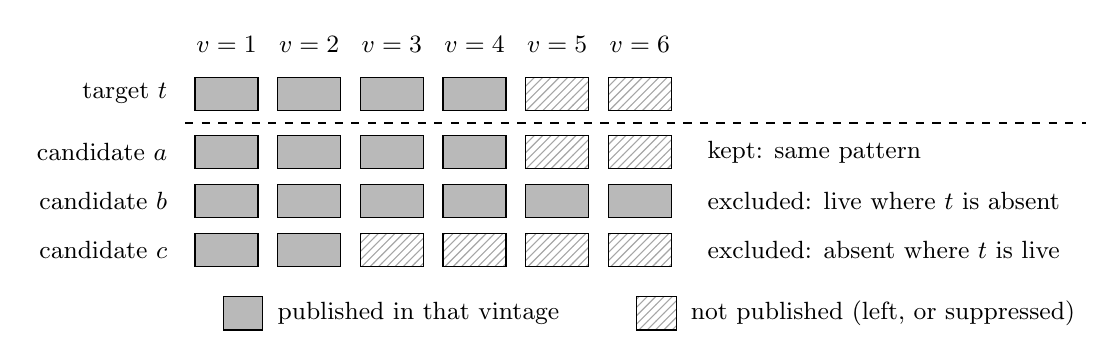
\begin{tikzpicture}[x=1.05cm,y=0.62cm,font=\small,
  live/.style={draw,fill=gray!55,minimum width=0.8cm,minimum height=0.42cm},
  gone/.style={draw,pattern=north east lines,pattern color=gray!70,minimum width=0.8cm,minimum height=0.42cm},
  lab/.style={anchor=east}]
  % header
  \foreach \m in {1,...,6} {\node at (\m,1) {$v=\m$};}
  % target
  \node[lab] at (0.4,0) {target $t$};
  \foreach \m/\s in {1/live,2/live,3/live,4/live,5/gone,6/gone} {\node[\s] at (\m,0) {};}
  % candidates
  \node[lab] at (0.4,-1.2) {candidate $a$};
  \foreach \m/\s in {1/live,2/live,3/live,4/live,5/gone,6/gone} {\node[\s] at (\m,-1.2) {};}
  \node[lab] at (0.4,-2.2) {candidate $b$};
  \foreach \m/\s in {1/live,2/live,3/live,4/live,5/live,6/live} {\node[\s] at (\m,-2.2) {};}
  \node[lab] at (0.4,-3.2) {candidate $c$};
  \foreach \m/\s in {1/live,2/live,3/gone,4/gone,5/gone,6/gone} {\node[\s] at (\m,-3.2) {};}
  % verdicts
  \node[anchor=west] at (6.7,-1.2) {kept: same pattern};
  \node[anchor=west] at (6.7,-2.2) {excluded: live where $t$ is absent};
  \node[anchor=west] at (6.7,-3.2) {excluded: absent where $t$ is live};
  \draw[dashed] (0.5,-0.6) -- (11.4,-0.6);
  % legend
  \node[live,minimum width=0.5cm] (l1) at (1.2,-4.5) {};
  \node[anchor=west] at (1.5,-4.5) {published in that vintage};
  \node[gone,minimum width=0.5cm] (l2) at (6.2,-4.5) {};
  \node[anchor=west] at (6.5,-4.5) {not published (left, or suppressed)};
\end{tikzpicture}
\caption{How the pooled adversary uses a loan's history. All four loans share the
target's key cell. An adversary who knows the vintages in which the target is
live keeps only candidates whose pattern of appearances matches the target's in
every vintage, and then ranks the survivors by its exposure readings
(Algorithm~\ref{alg:attack}). Shade and hatching both mark the two states, so the
figure reads in black and white.}
\label{fig:history}
\end{figure}

\begin{algorithm}[t]
\caption{Full-likelihood linkage attack on a programme of releases}\label{alg:attack}
\begin{algorithmic}[1]
\Require target $t$ with key $K(t)$; releases $D_1,\ldots,D_V$ with a persistent pseudonym;
  readings $y_r$ of $\log$ exposure with declared error $\sigma$, $r\in R$, where $R$ holds
  one reading or one per vintage in which $t$ is live; history
  $h_v(t)=\mathbf 1\{t\in D_v\}$ if the scenario grants it
\State $C\gets\{a\in D_1: K(a)=K(t)\}$ \Comment{candidates in the target's key cell}
\For{$a\in C$}
  \State $s(a)\gets\sum_{r\in R}\log\phi\bigl((y_r-\log e_a)/\sigma\bigr)$ \Comment{published exposure $e_a$}
  \If{the scenario grants the history}
    \For{$v=2,\ldots,V$}
      \If{$\mathbf 1\{a\in D_v\}\ne h_v(t)$} $s(a)\gets s(a)-30$ \Comment{mismatch in either direction}
      \EndIf
    \EndFor
  \EndIf
\EndFor
\State $M\gets\arg\max_{a\in C}s(a)$; name $\hat a$ drawn uniformly from $M$
\State \Return success $\mathbf 1\{\hat a=t\}$
\end{algorithmic}
\end{algorithm}


Table \ref{tab:decomp} separates the two for the adversary with history, and
Table \ref{tab:robust} adds the adversary without it. Each entry in Table
\ref{tab:eval} rests on 4{,}000 simulated attacks against independently drawn
targets. Tables \ref{tab:credit} and \ref{tab:eval} compute the per-release
identification rate with two separate functions of the pipeline, and a check at
20{,}000 targets (\texttt{scripts/estimand\_check.py}) shows that they estimate
the same quantity: 0.076 against 0.081 at $k_{\min} = 5$, 0.070 against 0.069 at
$k_{\min} = 10$, and 0.056 against 0.054 at $k_{\min} = 20$, each difference
within two standard errors.

Three further attacks run against the same releases. The relationship attack names,
for each released borrower, the lender holding the largest share of that borrower's
key class, and is scored by the share of allegations that are true. The attribute
attack reads arrears status off a key class whose members agree, and is scored by
accuracy on the classes it is confident about. The differencing attack compares two
vintages of the same cell and claims a single arrival or departure whenever the
count moves by one, and is scored by how often exactly one loan moved.

\subsection{The policies compared}\label{sec:eval-policies}

Five loan-level policies enter the comparison. They are stylised versions of rules
described by \citet{hundepool2012}, not copies of any institution's practice:

\begin{itemize}
\item no suppression, the isolated-release baseline;
\item a threshold rule, which withholds a cell unless at least three lenders
  contribute to it; for magnitude tables such a rule is usually applied beside a
  dominance $(n,k)$ or $p\%$ rule \citep[ch.~4]{hundepool2012}, which we leave out;
\item the same rule with a heuristic secondary suppression (the row labelled
  complementary suppression), which also withholds the smallest surviving cell in
  each region so that a suppressed cell cannot be recovered from a published row
  total; it is not audited against the other margins, sector and size, and is not
  secondary suppression in the sense of \citet{cox1980} and
  \citet{fischetti2001};
\item $k$-anonymity on the borrower key at $k = 5$ and $k = 10$.
\end{itemize}

The pipeline also runs two releases of noisy counts; we do not compare them with
the loan-level policies, because their targets are key classes rather than loans
and so their success event differs. Utility is the same weighted loss across
credit growth, concentration, the arrears ratio and lender-level supervision that
Section \ref{sec:credit} used, computed on what each policy actually publishes.

\begingroup\let\small\footnotesize\setlength{\tabcolsep}{4pt}\begin{table}[t]
\centering
\caption{Attack outcomes by protection policy, on the same credit register and the same adversary. The release and pooled columns give the share of targets the maximum-posterior linkage names correctly, for one release and pooled over the 6 vintages. Precision is measured over the attempts the adversary acts on, those whose posterior passes 0.5, and the column headed acts is how often it acts at all. The last two columns use the same success event as the release column for the size class with the highest rate, with that class's exact 95 per cent upper bound; a release passes the subgroup control when every class's bound meets the tolerance, which needs no correction for the number of classes. Utility is the negative weighted loss on the four analyses the register is collected for. Noisy-count releases are not compared: their targets are key classes, not loans.}
\label{tab:eval}
\small
\begin{tabular}{lrrrrrrrr}
\toprule
Policy & Kept & Utility & Release & Pooled & Precision & Acts & Worst class & Upper \\
\midrule
no suppression & 27{,}167 & -0.000 & 0.089 & 0.260 & 0.716 & 0.020 & 0.248 & 0.297 \\
three contributors & 27{,}068 & -0.019 & 0.084 & 0.255 & 0.822 & 0.018 & 0.180 & 0.228 \\
complementary suppression & 27{,}027 & -0.028 & 0.080 & 0.259 & 0.746 & 0.015 & 0.156 & 0.203 \\
$k$-anonymity, $k=5$ & 26{,}885 & -0.050 & 0.074 & 0.269 & 0.771 & 0.012 & 0.183 & 0.234 \\
$k$-anonymity, $k=10$ & 26{,}019 & -0.139 & 0.070 & 0.244 & 0.800 & 0.009 & 0.141 & 0.193 \\
\bottomrule
\end{tabular}
\end{table}
\endgroup

\subsection{What the attacks achieve}\label{sec:eval-results}

Table \ref{tab:eval} gives four results.

First, every suppression policy reduces the per-release risk and none of them
removes it. With no suppression the adversary names the right loan for
0.089 of targets. The threshold rule brings that to
0.084, $k$-anonymity at $k=5$ to 0.074, and at $k=10$ to
0.070. The reduction within a release is modest, because the exposure reading
separates candidates inside a cell however large the cell is. Every policy meets
the tolerance of 0.12 on one release.

Second, the same policies do far less against the pooled attack. Pooled over the
programme, the five policies lie between 0.244 and 0.269, and no suppression is
at 0.260. Under $k=5$ the per-release figure of 0.074 becomes 0.269 once the
adversary combines the vintages, and under $k=10$ it becomes 0.244. The largest
gap in the table, 0.195, belongs to $k$-anonymity, $k=5$. Table \ref{tab:decomp}
shows where the gap comes from. Under no suppression, six readings of exposure
against one release raise the rate from 0.089 to 0.158, and pooling the six
vintages with a single reading raises it to 0.191, with an upper bound of 0.201,
above the tolerance of 0.12. With both the rate is 0.260, so on this register the
two effects add with almost no interaction. The pooled attacks in this table know
the loan's history. For that adversary the programme finding does not rest on
the extra readings: with the same exposure reading as the per-release attack,
pooling alone takes the release above the tolerance. Without the history pooling
adds nothing (Section \ref{sec:eval-programme}).

\begingroup\let\small\scriptsize\setlength{\tabcolsep}{2pt}\begin{table}[t]
\centering
\caption{Where the pooled excess comes from. Share of targets named correctly, with the exact 95 per cent upper bound in brackets. The adversary attacks one release or all 6 vintages, holding one exposure reading or one per vintage (6). The first and last columns are the release and pooled columns of Table~\ref{tab:eval}; the middle two change one factor at a time on the same targets.}
\label{tab:decomp}
\small
\begin{tabular}{lrrrr}
\toprule
Policy & One release, one reading & One release, 6 readings & All releases, one reading & All releases, 6 readings \\
\midrule
no suppression & 0.089 (0.097) & 0.158 (0.168) & 0.191 (0.201) & 0.260 (0.272) \\
$k$-anonymity, $k=5$ & 0.074 (0.081) & 0.141 (0.150) & 0.183 (0.194) & 0.269 (0.281) \\
$k$-anonymity, $k=10$ & 0.070 (0.076) & 0.130 (0.139) & 0.179 (0.190) & 0.244 (0.256) \\
\bottomrule
\end{tabular}
\end{table}
\endgroup

Third, the adversary is often right when it acts, but it seldom acts on one
release. Under $k=5$ it passes the decision threshold on 0.012 of its attempts
and is right on 0.771 of those: 48 of 4{,}000 attempts pass, and 37 of them are
right. That is about 108 attempts per correct identification, and the precision
rests on 48 decisions, so it is loosely measured. An evaluation that reports only
the average success rate hides the precision, and one that reports only the
precision hides how few attempts it rests on.

Fourth, the average conceals a subgroup. The last two columns of Table
\ref{tab:eval} use the same success event as the release column, that the
highest-scoring candidate is the target, for the size class with the highest
rate, with that class's own exact upper bound. The release passes the subgroup
control only if every class's bound meets the tolerance, an intersection--union
test that needs no correction for the number of classes (Section \ref{sec:gov}).
With no suppression the largest-firm class reaches 0.248, with an upper bound of
0.297; under $k=5$ it reaches 0.183 (0.234), and under $k=10$ 0.141 (0.193). No
row of the table passes the subgroup control at 0.12 even on a single release.
Large borrowers are few, so their key classes are small and their exposures are
far apart, and both effects push the same way.

The other three attacks are largely indifferent to the lever. Under $k=5$ an alleged
borrower-lender relationship is true 0.324 of the time, and a unit change between
vintages is a single loan movement 0.623 of the time. A confident reading of
arrears status is right 0.946 of the time, but guessing no arrears for every loan
is right 0.929 of the time, so the gain over the base-rate guess is 0.017 and the
attack discloses little. Every homogeneous class on this register is homogeneous
in the benign direction (Section \ref{sec:credit}), so in the harmful direction it
discloses nothing here. Suppression on the borrower key is aimed at identification,
and it does not touch the disclosures that do not require it.

\subsection{Per-release calibration against programme calibration}\label{sec:eval-programme}

Fix the tolerance at 0.12 and choose the minimum cell count by the exact upper
bound, as rule \eqref{eq:admiss} requires, not by the point estimate. The level is
chosen from a grid by the same bounds that certify it, so we use fixed-sequence
testing (Proposition \ref{prop:fixedseq}): the levels are tested from $k_{\min} =
300$ down, the procedure stops at the first level whose bound exceeds 0.12, and
the floor is the last level that passed. The choice uses one draw of 4{,}000
targets at each level. The chosen level is then audited on a second, independent
draw, and that confirmation is the figure a decision record should carry; where
it fails, the next stricter level is confirmed on the same fresh draw, which stays
valid for the reason given after Proposition \ref{prop:fixedseq}. Table
\ref{tab:robust} gives the result for six adversaries, which differ in the
vintages, the readings, the history and the precision they hold, and it reports
the cost of each floor in loans and in exposure. Algorithm \ref{alg:selection}
sets out the selection and confirmation steps as they were run, and Example
\ref{ex:selection} carries them through for one adversary; the error bound
rests on the selection step, and the confirmation draw only guards against
reporting a floor that passed by chance near the tolerance.

\begin{algorithm}[t]
\caption{Fixed-sequence choice of a floor, with confirmation}\label{alg:selection}
\begin{algorithmic}[1]
\Require floors $k_1>k_2>\cdots>k_L$ fixed in advance; tolerance $\tau$; level $\alpha$;
  two independent target draws of size $B$
\State $\hat k\gets\text{none}$
\For{$\ell=1,\ldots,L$} \Comment{selection draw}
  \State run the declared attack on $B$ fresh targets at $k_\ell$; $Y\gets$ successes
  \If{$\overline R(Y,B;\alpha)>\tau$} \textbf{break} \Comment{first failure ends the search}
  \EndIf
  \State $\hat k\gets k_\ell$
\EndFor
\If{$\hat k\ne\text{none}$} \Comment{confirmation draw}
  \For{each $k\ge\hat k$ in increasing order}
    \State run the attack on $B$ new targets at $k$; $Y'\gets$ successes
    \If{$\overline R(Y',B;\alpha)\le\tau$} \Return $k$ with its confirmed bound
    \EndIf
  \EndFor
\EndIf
\State \Return none \Comment{no tested floor meets the tolerance}
\end{algorithmic}
\end{algorithm}


\begin{table}[t]
\centering
\caption{What sets the programme floor on the synthetic credit register, tolerance 0.12. History: the adversary knows in which vintages the target's loan is live. The floor is chosen by fixed-sequence testing from $k=300$ down on one draw of 4{,}000 targets and confirmed on a second, independent draw (rate, with exact 95 per cent upper bound); where confirmation fails the next stricter level that passes is shown. Loans and exposure are the percentages of the first release kept at that floor. The subgroup floor requires every size class to meet the tolerance, with the largest firms on a stratified draw, from $k=200$ down. The insider reads exposure with error 0.01 on the log scale. In the Floor column ``none'' means no level up to 300 passes, and in the Subgroup column no level up to 200.}
\label{tab:robust}
\small\setlength{\tabcolsep}{3pt}
\begin{tabular}{lrrrrr}
\toprule
Adversary & Floor & Confirmation & Loans (\%) & Exposure (\%) & Subgroup \\
\midrule
One release, one reading & 1 & 0.084 (0.092) & 100 & 100 & 20 \\
Six releases, one reading, no history & 1 & 0.083 (0.091) & 100 & 100 & -- \\
Six releases, one reading, history & 75 & 0.096 (0.104) & 45 & 11 & 200 \\
Six releases, reading per vintage, no history & 20 & 0.105 (0.114) & 85 & 52 & -- \\
Six releases, reading per vintage, history & 150 & 0.101 (0.109) & 20 & 4 & none \\
Insider: exact exposure, history & none & -- & -- & -- & -- \\
\midrule
\multicolumn{6}{l}{\emph{Exposure published to one significant figure}}\\
One release, one reading & 1 & 0.079 (0.086) & 100 & 100 & -- \\
Six releases, one reading, history & 50 & 0.111 (0.119) & 58 & 20 & -- \\
Six releases, reading per vintage, history & 150 & 0.085 (0.092) & 20 & 4 & -- \\
Insider: exact exposure, history & none & -- & -- & -- & -- \\
\bottomrule
\end{tabular}
\end{table}


Against one release with one exposure reading, the floor is 1: no suppression, all
27{,}167 loans of the first release kept, and a confirmation rate of 0.084 with an
upper bound of 0.092. Pooling the six releases with the same single reading, for
an adversary that does not know in which vintages the target's loan is live, adds
nothing: the floor stays at 1 and the confirmation is 0.083 (0.091). The reason is
structural, and it is stated in Proposition \ref{prop:nohistory} below.

The adversary that knows the history needs more. Selection passes at 50, but
confirmation there fails, at 0.115 with an upper bound of 0.123, so the floor is
the next stricter level, 75, confirmed at 0.096 (0.104). This is the floor that
pooling alone requires, with the auxiliary data of the per-release attack plus
the history. An adversary that holds one reading per live vintage but not the
history needs 20 (confirmation 0.105, bound 0.114). The full attack, the pooled
attack of Table \ref{tab:eval}, with a reading per live vintage and the history,
needs 150, confirmed at 0.101 (0.109). The insider fails at every level: its
success is 0.772 at $k_{\min} = 1$ and still 0.416 at $k_{\min} = 300$, because a
precise reading of exposure separates candidates in any cell.

When several adversaries are declared for one release, the floor must meet the
tolerance for all of them at once. The companion article does this with a release
chain, shown in Figure \ref{fig:chain} and stated in Algorithm \ref{alg:chain}:
the floors are audited from the strictest down, each declared attack at each
floor is a coordinate of the registered betting gate at the full error level, and
the chain stops at the first floor at which any attack fails. Because a floor
that fails ends the search, no split of $\alpha$ over floors or attacks is needed.
Figure \ref{fig:chain} shows the pattern most streams followed on this register:
the three attacks certify down to $k_{\min} = 150$, and at 100 the full pooled
attack, whose risk there is 0.116, does not certify within the cap of 3{,}000
draws, so the chain chooses 150.

\begin{figure}[t]
\centering
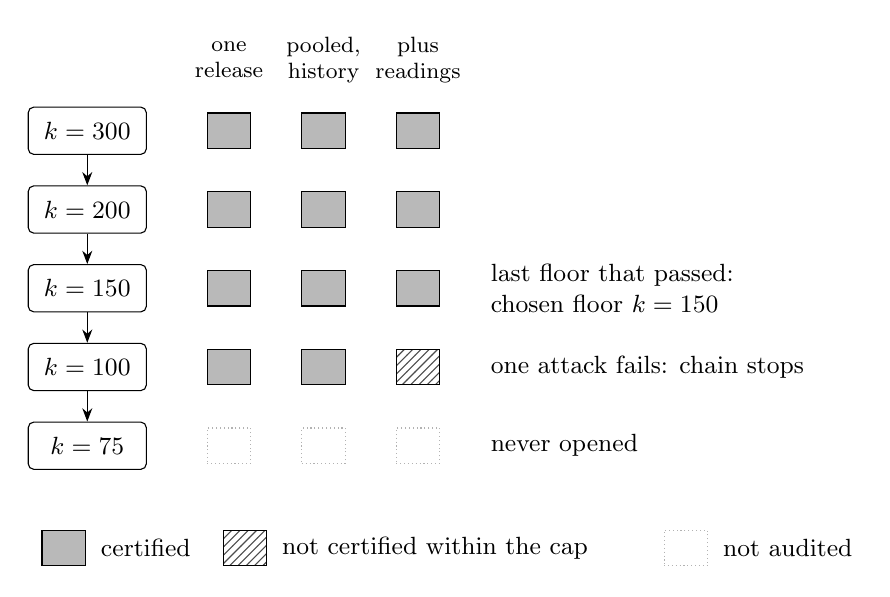
\begin{tikzpicture}[font=\small,
  floor/.style={draw,rounded corners=2pt,minimum width=1.5cm,minimum height=0.6cm},
  coord/.style={draw,minimum width=0.55cm,minimum height=0.45cm,inner sep=1pt},
  pass/.style={coord,fill=gray!55},
  fail/.style={coord,pattern=north east lines,pattern color=black!70},
  skip/.style={coord,draw=gray!60,densely dotted},
  >=Stealth]
  \foreach \k/\y in {300/0,200/-1,150/-2,100/-3,75/-4} {
    \node[floor] (f\k) at (0,\y) {$k=\k$};
  }
  % components: single, pooled-history, full
  \foreach \k/\y/\a/\b/\c in {300/0/pass/pass/pass,200/-1/pass/pass/pass,150/-2/pass/pass/pass,100/-3/pass/pass/fail,75/-4/skip/skip/skip} {
    \node[\a] at (1.8,\y) {};
    \node[\b] at (3.0,\y) {};
    \node[\c] at (4.2,\y) {};
  }
  \node[align=center,font=\footnotesize] at (1.8,0.9) {one\\release};
  \node[align=center,font=\footnotesize] at (3.0,0.9) {pooled,\\history};
  \node[align=center,font=\footnotesize] at (4.2,0.9) {plus\\readings};
  \foreach \a/\b in {300/200,200/150,150/100,100/75} {\draw[->] (f\a) -- (f\b);}
  \node[anchor=west,align=left] at (5.0,-2) {last floor that passed:\\ chosen floor $k=150$};
  \node[anchor=west,align=left] at (5.0,-3) {one attack fails: chain stops};
  \node[anchor=west,align=left] at (5.0,-4) {never opened};
  % legend
  \node[pass] at (-0.3,-5.3) {}; \node[anchor=west] at (0.05,-5.3) {certified};
  \node[fail] at (2.0,-5.3) {}; \node[anchor=west] at (2.35,-5.3) {not certified within the cap};
  \node[skip] at (7.6,-5.3) {}; \node[anchor=west] at (7.95,-5.3) {not audited};
\end{tikzpicture}
\caption{A release chain chooses the cell-count floor. Floors are audited from the
strictest down; at each floor every declared attack is a coordinate audited on
fresh targets at the full error level, and the floor passes only if all of them
certify. The chain stops at the first floor that fails and chooses the last one
that passed (Algorithm~\ref{alg:chain}). The pattern shown is the one most streams
followed in the credit-register audit of the companion article.}
\label{fig:chain}
\end{figure}

\begin{algorithm}[t]
\caption{Release chain with the registered betting gate}\label{alg:chain}
\begin{algorithmic}[1]
\Require floors $k_1>\cdots>k_L$ and declared attacks $a_1,\ldots,a_J$, both fixed before
  any outcome; tolerance $\tau$; chain weight $w$; bet cap $c<\tau$; draw cap $B$
\State register the chain in the programme ledger, spending $w$ once
\State $\hat k\gets\text{none}$
\For{$\ell=1,\ldots,L$}
  \For{$j=1,\ldots,J$} \Comment{open coordinate $(k_\ell,a_j)$ only now}
    \State $\log E\gets0$; $Y\gets0$
    \For{$b=1,\ldots,B$}
      \State $q\gets\min\{(Y+\tfrac12)/b,\,c\}$ \Comment{bet fixed before the outcome}
      \State draw a fresh target; $X\gets$ success of $a_j$ at $k_\ell$
      \State $\log E\gets\log E+X\log(q/\tau)+(1-X)\log\{(1-q)/(1-\tau)\}$; $Y\gets Y+X$
      \If{$\log E\ge\log\{1/(\alpha w)\}$} mark certified; \textbf{break}
      \EndIf
    \EndFor
    \If{not certified} \Return $\hat k$ \Comment{the floor fails; stop the chain}
    \EndIf
  \EndFor
  \State $\hat k\gets k_\ell$ \Comment{every declared attack certified}
\EndFor
\State \Return $\hat k$
\end{algorithmic}
\end{algorithm}


The cost of these floors falls on credit volume more than on loan counts. Large
firms carry the largest exposures and sit in the thinnest cells, so they are the
first to go. The floor of 75 keeps 45 per cent of loans but 11 per cent of
exposure, and the floor of 150 keeps 20 per cent of loans, 4 per cent of exposure
and no loan to a large firm; no large-firm loan survives any floor from 75 up.
Even the floor of 50 that selection first picked for the history adversary keeps
58 per cent of loans and 20 per cent of exposure. A file that meets the
tolerance against a history-aware adversary is therefore not the file its users
asked for: it has lost the borrowers that concentration and supervisory
analysis are about. Against such an adversary a loan-level release is the wrong
product. Aggregates with a contributor rule (Section \ref{sec:credit}), or access
to the loan-level file in a secure setting under the Five Safes
\citep{desai2016}, where the declared adversary no longer holds the file, are the
realistic options. The loan-level file of this section stands in for two real
products: the loan-level disclosures that accompany securitisations, and research
files as an accredited user sees them.

The subgroup control asks more. When every size class must meet the tolerance, with
the largest-firm class audited on its own stratified draw of 4{,}000 targets
because a uniform draw gives it too few, the per-release floor is 20, pooling with
the history needs 200, and for the full attack no level up to 200 passes. The
grid for this control starts at 200, because at 300 the classes that remain are
too thin to audit. From $k_{\min} = 75$ no loan of the largest class is released,
and that class then has no target to protect, so the subgroup floors above 75
are set by the other classes. These subgroup floors were chosen by the same
fixed-sequence rule but not confirmed on a second draw. Under the supremum control
the per-release answer is therefore 20, not 1, and a programme needs far more.

Two further rows of Table \ref{tab:robust} publish exposure rounded to one
significant figure. The outside adversaries barely notice: their floors are 1, 50
and 150. The insider still fails at every level, but its success at $k_{\min} = 1$
halves, to 0.388, because rounding creates ties among candidates that a precise
reading can no longer break.

\paragraph{The floor depends on the tolerance.} Table \ref{tab:tolerance-floors}
repeats the selection at three other tolerances, from the same draw. At 0.05 the
per-release floor is 40, pooling with the history needs 300 and the full attack
has no floor up to 300; at 0.20 the three floors are 1, 5 and 30. The column for
pooling with the history shows the selection result, 50 at a tolerance of 0.12,
before the confirmation that moved it to 75. A committee that is unsure of its
tolerance should read the whole table, since the floor moves by an order of
magnitude across this range.

\begin{table}[t]
\centering
\caption{The floor chosen at four tolerances by the selection draw of Table~\ref{tab:robust}, before confirmation; at 0.12 pooling with the history therefore shows 50, where Table~\ref{tab:robust} shows the confirmed 75. ``None'' means no level up to 300 passes.}
\label{tab:tolerance-floors}
\small
\begin{tabular}{lrrrr}
\toprule
Tolerance & One release & Pooling, history & Full pooled & Insider \\
\midrule
0.05 & 40 & 300 & none & none \\
0.09 & 5 & 100 & 200 & none \\
0.12 & 1 & 50 & 150 & none \\
0.20 & 1 & 5 & 30 & none \\
\bottomrule
\end{tabular}
\end{table}


\paragraph{A chain of audits.} The companion article runs the same choice as one
release chain: a fixed sequence of intersection--union tests, each at the full
level $\alpha$, with all three outside attacks declared as coordinates. Over 20
independent target streams it chose 150 in 19 and 100 once, against an estimated
true floor of 100, and no stream chose a floor that was unsafe. The floor of 150
is thus what an honest audit of this register returns. The gap to 100 comes from
the full attack's risk at that floor, 0.116, which lies so close to the tolerance
that the audit's capped bet certifies it only by chance.

\begin{proposition}[Without the history, the other vintages are uninformative]\label{prop:nohistory}
Suppose that each loan's published key and exposure are the same in every vintage
in which it is released, that whether a loan is live in a vintage is drawn
independently of its key, its exposure and the adversary's auxiliary information,
and that the adversary knows only that the target is live in the first release.
Then, for any fixed auxiliary information, the posterior over candidates computed
from all $m$ releases equals the posterior computed from the first release, and the
pooled attack succeeds exactly when the single-release attack does.
\end{proposition}

\begin{proof}
The candidates are the loans live in the first release whose key agrees with the
target's. Let $Z$ be the auxiliary information and write $L_j$ for the vector of
live indicators of candidate $j$ over vintages $2, \dots, m$. Under the hypothesis
$H_j$ that $j$ is the target, the other vintages add to the likelihood only the
published key and exposure of each candidate, which repeat those of the first
release, and the factor $\prod_\ell \Prob(L_\ell)$. By assumption the law of
$L_\ell$ does not depend on which candidate is the target, and the adversary holds
nothing that ties $Z$ to any $L_\ell$, so the factor is the same under every $H_j$
and cancels from the posterior \eqref{eq:post}. What remains is the first-release
likelihood of $Z$, so the two posteriors, and their maximisers, coincide.
\end{proof}

The proposition explains the second row of Table \ref{tab:robust}, and it holds on
this register by construction of the generator: published values do not change
between vintages, and whether a loan is live is drawn independently of them. It
shows where the gain from pooling lives here: in the history, not in the
releases. On a register where published fields change from month to month, for
example where outstanding exposure is published and amortises, the other vintages
would carry information of their own, and the proposition would not apply.

\paragraph{Replication over register draws.} Every figure so far comes from one
register draw with one reading noise. Table \ref{tab:replication} repeats the
choice over 20 independent register draws and three values of the standard
deviation of the adversary's log-exposure reading, with 2{,}000 targets per level.
At the value of the main study, 0.6, the per-release floor is 1 in every draw,
pooling with the history gives a median of 75 (range 40 to 75) and the full
attack 150 (range 100 to 150). With a reading twice as precise, at 0.3, the
medians are 20, 150 and 300, and for the full attack no level up to 300 passes in
3 of the 20 draws. At 1.0 they are 1, 40 and 75. The adversary's reading
precision moves the floor more than anything else we varied, and it is the input
an institution most needs to argue for. For the full attack at $k_{\min} = 150$
the rate has a between-register standard deviation of 0.0073 over the 20 draws.
We computed a 95 per cent interval for it from the chi-square law with 19 degrees
of freedom, which runs from 0.006 to 0.011. The binomial standard error of one
draw of 2{,}000 targets at the mean rate is 0.0064, inside that interval, so the
register draw may add nothing or may add a design standard deviation of up to
about 0.009. Twenty draws do not estimate the design term well. What they do show
is that at fixed precision the floor stays in a narrow band across register
draws, from 40 to 75 for pooling with the history and from 100 to 150 for the
full attack.

% the generated table writes a text-mode >, which the OT1 encoding prints as an inverted question mark
\begingroup\let\small\scriptsize\setlength{\tabcolsep}{4pt}\begin{table}[t]
\centering
\caption{The floor over 20 independent register draws and three levels of reading noise (the standard deviation of the adversary's log-exposure reading), 2{,}000 targets per level. Median floor, with the smallest and largest in brackets; ``none'' means no level up to 300 passed, and a superscript counts the register draws in which that happened.}
\label{tab:replication}
\small
\begin{tabular}{lrrr}
\toprule
Reading SD & One release, one reading & Six releases, one reading, history & Six releases, reading per vintage, history \\
\midrule
0.3 & 20 [10, 20] & 150 [150, 200] & 300 [300, none]$^{3}$ \\
0.6 & 1 [1, 1] & 75 [40, 75] & 150 [100, 150] \\
1 & 1 [1, 1] & 40 [30, 40] & 75 [50, 100] \\
\bottomrule
\end{tabular}
\end{table}
\endgroup

\paragraph{Rotating the pseudonym.} The attacks match loans across vintages
through a pseudonym that persists. If the pseudonym rotated each month, the
adversary would have to relink vintages through the published fields. With
exposure published exactly, the pair of key and exposure is unique for every
first-release loan at every floor tested (a share of 1.000), so the published
fields alone relink every loan and rotation gives no protection. With exposure
rounded to one significant figure the pair relinks 0.104 of loans at $k_{\min} =
1$, so rotation would then remove most of the relinkage that the persistent
pseudonym gives. Rotation is a control on linkability, not pseudonymisation in
the sense of the data protection law (Remark \ref{rem:finer}), and the pseudonym
should be a keyed hash under a key held apart from the release team. We did not
rerun the attacks with rotation; the relink share is a count of loans that could
be joined, not an attack.

This is the practical content of Proposition \ref{prop:nopool}. The proposition
denies that any function of the marginals can bound the pooled risk, and the
evaluation shows what that denial costs on a synthetic monthly collection with
a lever supervisors recognise. Among the policies in Table \ref{tab:eval}, none
calibrated on one release meets the tolerance against the pooled attack with
history, while each passes its own test at vintage 1. A floor chosen by
fixed-sequence testing on the declared pooled adversary does meet it (Table
\ref{tab:robust}). Which floor that is depends on what the institution declares
the adversary to know: 1 without the history, 75 with it, 150 with a reading in
every vintage as well, none for an insider, and more again if every size class
must be protected.

\subsection{The neural release pipeline}\label{sec:eval-neural}

The release chain needs a bet for every draw and a floor at which to start. The
neural release pipeline supplies both from a network, and it is the package's main
entry point (\texttt{python -m privacy\_risk.neural\_pipeline}). Figure
\ref{fig:neural-pipeline} shows its four stages and Algorithm \ref{alg:neural}
states them. The declared attacks are first run on a dense grid of 25 floors with
400 development targets each, on seeds the final audit never uses. A network with
two hidden layers of 16 units is fitted to these counts by the binomial
likelihood, one output per declared attack, with a third of the floors held out
for early stopping; a logistic model is fitted to the same counts as a baseline.
The features are those an agency can compute from the register without running an
attack: the floor, the share of loans kept, the mean size of the released cells
and the share of released loans not live in every vintage. Before any final
outcome exists, the fitted model predicts every attack's success at every floor of
the release grid, and the plan (the bets, and a start floor one step stricter than
the floor the model predicts to be safe) is frozen with its digest. The release
chain then audits the plan on fresh targets. If it fails at its first floor, a
reserve of a fifth of the error budget runs a second chain from $k_{\min} = 300$.

Because every bet is fixed before its outcome and the chain's order is fixed at
registration, the network's accuracy does not enter the error bound: a poor model
costs attacks and cannot raise the chance of certifying an unsafe floor. Table
\ref{tab:neural-pipeline} compares five designs on the same final draws. Every
design chose the same floor as the release chain with running-rate bets in almost
every stream, 150, and none chose an unsafe floor. The difference is cost. With
bets from the network the chain used a median of 5{,}620 attacks against 6{,}422
with running-rate bets, and with the network's start floor as well it used 5{,}044,
about a fifth fewer, and never needed the reserve. Depth does not explain the
saving. The logistic model's predictions were closer to the estimated true risks
(mean absolute error 0.004 against 0.008 for the network), and its plan saved as
many attacks; the gain comes from basing bets and the start on development
evidence rather than on the network's hidden layers. The network is kept as the
pipeline's default because its architecture extends to many more features and
declared attacks than this register has, and the logistic model is reported
beside it so that a reader can see when depth has not paid.

\begin{figure}[t]
\centering
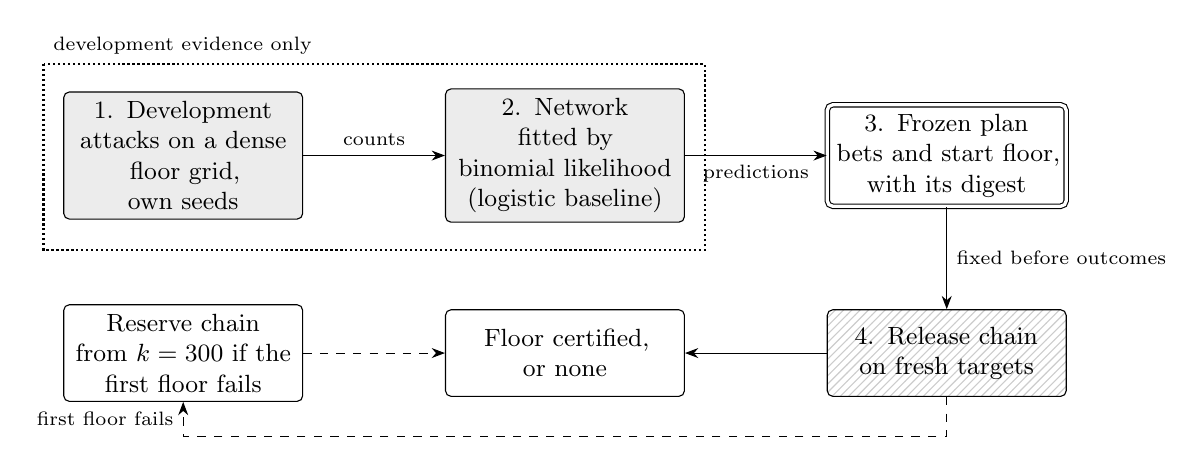
\begin{tikzpicture}[font=\small,node distance=0.5cm and 1.8cm,
  stage/.style={draw,rounded corners=2pt,align=center,text width=2.8cm,minimum height=1.1cm},
  dev/.style={stage,fill=gray!15},
  final/.style={stage,pattern=north east lines,pattern color=gray!40},
  frozen/.style={stage,double,double distance=1.2pt},
  >=Stealth]
  \node[dev] (a) {1. Development\\attacks on a dense\\floor grid, own seeds};
  \node[dev,right=of a] (b) {2. Network fitted by\\binomial likelihood\\(logistic baseline)};
  \node[frozen,right=of b] (c) {3. Frozen plan\\bets and start floor,\\with its digest};
  \node[final,below=1.3cm of c] (d) {4. Release chain\\on fresh targets};
  \node[stage,left=of d] (e) {Floor certified,\\or none};
  \node[stage,left=of e] (f) {Reserve chain\\from $k=300$ if the\\first floor fails};
  \draw[->] (a) -- node[above,font=\scriptsize]{counts} (b);
  \draw[->] (b) -- node[below,font=\scriptsize]{predictions} (c);
  \draw[->] (c) -- node[right,font=\scriptsize]{fixed before outcomes} (d);
  \draw[->] (d) -- (e);
  \draw[->,dashed] (d.south) -- ++(0,-0.5) -| node[near end,left,font=\scriptsize]{first floor fails} (f.south);
  \draw[->,dashed] (f) -- (e);
  \draw[densely dotted,thick] ($(a.north west)+(-0.25,0.35)$) rectangle ($(b.south east)+(0.25,-0.35)$);
  \node[anchor=south west,font=\scriptsize] at ($(a.north west)+(-0.25,0.35)$) {development evidence only};
\end{tikzpicture}
\caption{The neural release pipeline. Grey boxes use development attacks only;
the double box is the plan, frozen with its digest before any final outcome
exists; the hatched box is the only stage whose outcomes can certify a floor. The
network's predictions choose the bets and the floor at which the release chain
starts, so a poor network costs attacks but cannot raise the chance of certifying
an unsafe floor.}
\label{fig:neural-pipeline}
\end{figure}

\begin{algorithm}[t]
\caption{The neural release pipeline}\label{alg:neural}
\begin{algorithmic}[1]
\Require declared attacks $a_1,\ldots,a_J$; release grid $k_1>\cdots>k_L$; tolerance
  $\tau$; level $\alpha$; reserve share $\omega$; bet cap $c<\tau$
\State run each $a_j$ on $n$ development targets at every floor of a dense grid, on
  seeds the final audit never uses; record counts $K_{kj}$ \Comment{stage 1}
\State compute features $x_k$ of each floor from the register alone (floor, share
  kept, mean cell size, share of loans not live in every vintage)
\State fit $f_\theta$ by the binomial log likelihood of $K_{kj}$ out of $n$, with
  held-out floors for early stopping \Comment{stage 2}
\State $\hat r_{kj}\gets f_\theta(x_{k})_j$ for the release grid; $q_{kj}\gets\min\{\hat r_{kj},c\}$
\State $\hat k\gets$ last floor, from $k_1$ down, with $\max_j\hat r_{kj}<\tau$; start
  $k_s\gets$ the floor one step stricter than $\hat k$
\State freeze $\{q_{kj}\}$, $k_s$ and their digest in the ledger \Comment{stage 3}
\State run Algorithm~\ref{alg:chain} from $k_s$ down with weight $1-\omega$ and the frozen
  bets \Comment{stage 4}
\If{the chain fails at $k_s$}
  \State run Algorithm~\ref{alg:chain} from $k_1$ down with weight $\omega$
\EndIf
\State \Return the certified floor, or none
\end{algorithmic}
\end{algorithm}

\begin{table}[t]
\centering
\caption{The neural release pipeline on the synthetic credit register, 20 attack streams, tolerance 0.12, $\alpha=0.05$. Every design is a release chain over the three declared attacks on the same final draws; they differ only in where the bets and the start floor come from. The network and the logistic model are fitted to development attacks on separate seeds and fixed before the final audit. Entries give each floor chosen with the number of streams in brackets, and the median number of attacks.}
\label{tab:neural-pipeline}
\small
\begin{tabular}{lrr}
\toprule
Source of bets and start & Floor chosen & Attacks \\
\midrule
Running-rate bets, chain from 300 & 100 (1), 150 (19) & 6{,}422 \\
Logistic bets, chain from 300 & 100 (2), 150 (18) & 5{,}572 \\
Network bets, chain from 300 & 100 (2), 150 (18) & 5{,}620 \\
Logistic bets and start floor & 100 (1), 150 (19) & 5{,}019 \\
Network bets and start floor & 100 (1), 150 (19) & 5{,}044 \\
\bottomrule
\end{tabular}
\end{table}


Figure \ref{fig:neural-predictions} shows what the network learned. In each panel
the solid line is the network's prediction at the 13 floors of the release grid,
fixed before the final audit, and the dotted line is the true risk estimated from
100{,}000 separate targets per floor. The crosses are the development rates, each
from only 400 attacks, which is all the network saw. It recovers the shape of all
three curves: flat and low for a single release, and falling steeply with the floor
for the two pooled attacks, crossing the tolerance near $k_{\min} = 100$ for the
full pooled attack, which is where the true floor lies. Its largest errors are in
the middle of panel (c), where it follows the scatter of the development rates
more closely than the logistic model does. Table \ref{tab:neural-fit} puts numbers
on this. The two models reach almost the same held-out log loss, 0.3482 for the
network and 0.3480 for the logistic model, and both predict a floor of 100 and
start the chain at 150; the network's mean error against the true risks is 0.008
and the logistic model's 0.004. The network therefore fits the development data as
well as the simpler model and no better, and on this register its extra capacity
goes into following noise.

\begin{figure}[t]
\centering
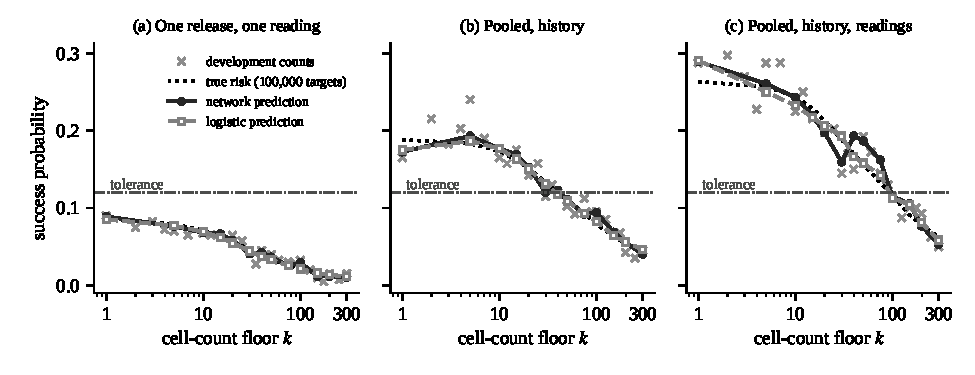
\includegraphics[width=\linewidth]{figures/fig_neural_predictions.pdf}
\caption{What the neural network predicted. For each declared attack, the frozen
predictions of the network (solid line, filled circles) and of the logistic model
(dashed line, open squares) against the true risk estimated from 100{,}000
separate targets (dotted line), with the development success rates the models were
fitted to (crosses, 400 targets each) and the tolerance (dash-dot line). The
network was fitted to the crosses alone and never saw the final audit.}
\label{fig:neural-predictions}
\end{figure}

\begin{table}[t]
\centering
\caption{What the two models learned from the development attacks. Log losses are the binomial log loss per development attack on the training and held-out floors; the epoch is where held-out loss was lowest. Errors compare each model's frozen prediction with the true risk, estimated from 100{,}000 separate targets, over the 39 coordinates of the release grid. The predicted floor is the last floor, from $k=300$ down, at which every predicted risk lies below the tolerance; the start floor is one step stricter.}
\label{tab:neural-fit}
\small\setlength{\tabcolsep}{4pt}
\begin{tabular}{lrrrrrrr}
\toprule
 & \multicolumn{2}{c}{Log loss} & & \multicolumn{2}{c}{Error against truth} & \multicolumn{2}{c}{Floor}\\
\cmidrule(lr){2-3}\cmidrule(lr){5-6}\cmidrule(lr){7-8}
Model & Training & Held out & Epoch & Mean & Largest & Predicted & Start \\
\midrule
Network, two hidden layers & 0.3240 & 0.3482 & 1146 & 0.008 & 0.031 & 100 & 150 \\
Logistic model & 0.3245 & 0.3480 & 2067 & 0.004 & 0.027 & 100 & 150 \\
\bottomrule
\end{tabular}
\end{table}


\subsection{What the attack needs, and a wrong model}\label{sec:eval-cost}

Appendix \ref{app:eval-extra} withdraws the adversary's auxiliary information one
field at a time (Table \ref{tab:ablation}). Without the exposure reading the
adversary never passes the decision threshold under $k$-anonymity at $k=5$; the
key narrows the candidates to a cell and the reading separates the members of
that cell, while neither does much alone. When the adversary misstates the
dispersion of its own reading, its success barely moves but its calibration gap
grows from 0.003 to as much as 0.073, which is what the falsification tests of
Section \ref{sec:falsify} are for.

\subsection{What this evaluation does not settle}\label{sec:eval-limits}

The register is synthetic, and every result in this section holds on the
synthetic register only. Its structure follows a supervisory collection, with
skewed lender shares, several relationships per large borrower and monthly entry and
exit, but the parameters are chosen, not estimated from a real credit register,
which cannot be released. Two simplifications bear on the floors. Exposure is
constant across vintages, so the other vintages carry no information without the
history (Proposition \ref{prop:nohistory}); with amortising balances they would.
And whether a loan is live is independent of its key and exposure, where in a
real register large loans may run longer. The results are therefore claims about
a class of release systems with these structural features, and the way to refute
them is to run the same evaluation inside an institution that holds the real
file. The pipeline's credit module would take the real register in place of the
simulated one, but it has not been run on a real register, and Section
\ref{sec:real} ran only the demographic path on real files.

The adversary is one adversary, strong in some respects and weak in others. It
holds the key exactly, uses a persistent pseudonym, knows the true error model of
its exposure reading and, in the pooled attacks with history, the loan's live
vintages. It does not use the arrears status, the lender identity or a longer
history. The evaluation is therefore neither a lower nor an upper bound on what an
adversary can achieve. Its value is comparative, since every policy faces the same
attacker, and conditional, since every floor holds for the adversary declared.

Finally, the evaluation compares policies as they are usually configured, not as
they could be. A minimum-contributor rule applied to the pooled programme rather
than to each vintage would do better than the row for it here: the same lever,
calibrated on the programme, changes the outcome.


\section{Falsification and validation}\label{sec:falsify}

Reproducing the equations of Sections \ref{sec:setup} to \ref{sec:dp} in
software is an implementation check, not empirical validation. Evidence for the
scenario model must be capable of contradiction. We propose six tests, each
with a stated failure consequence, and report how the simulation of Section
\ref{sec:sim} performs against them.

\begin{enumerate}
\item \textbf{Linkage calibration.} Posterior probabilities from \eqref{eq:post}
must agree with held-out match frequencies within prespecified bands. Figure
\ref{fig:calib} shows the test passing for the correct model with a mean gap of
0.007 and failing for a misspecified covariate precision with a gap of 0.049,
while the two risk estimates differ by 0.007. Failure means the risk figure is not
supported, whatever its value.

\item \textbf{Population-frequency validation.} The model behind
\eqref{eq:rho} must predict held-out or externally benchmarked key frequencies.
In Section \ref{sec:sim} the fitted law recovers the mean population cell size
to within 1 per cent and the uniqueness probability $\rho$ to between 8 and 25
per cent, and the direction of the error is conservative. The test also shows
misfit: the fitted dispersion drifts with the sampling fraction, from 0.33 to
0.51, where a negative binomial law closed under thinning would hold it fixed.
Failure means the model-based $\rho$ should be replaced by a bound. We act on
that here: the model-based figure enters no decision in this paper and is
reported only beside the truth, and on the census file, where there is no truth,
Section \ref{sec:real} reports $\rho$ across a range of sampling fractions
rather than as one value.

\item \textbf{Adversary stress test.} A materially stronger plausible feature
set must not push the upper risk bound above $\tau$. In the simulation, an adversary whose
covariate is twice as precise raises the simulated risk by between 1 and 76 per
cent across the 45 settings of the grid, with a median of 40 per cent. This is
why the robust risk \eqref{eq:rob}, and not the nominal risk, is the coordinate
in Figure \ref{fig:frontier}. Capability and modelling are separate things, and
a second check records the difference: an adversary that keeps its information
but assumes the covariate is noisier than it is loses only 0.007 of its success
rate while its calibration gap grows sevenfold, so a risk figure alone will not
reveal the mistake. The record swapping lever described in Section
\ref{sec:sim} was removed on the same principle. Failure of the test means the
release fails or the scenario is revised in writing.

\item \textbf{Mechanism monotonicity.} Where stronger protection is claimed to
reduce risk, violations must be investigated rather than smoothed. Every row of
Table \ref{tab:kanon} violates the nominal bound on the supremum control, and
the investigation of that violation is Proposition \ref{prop:kanon}. Three breaks
in order also appear. The worst target in Table \ref{tab:kanon} rises from 0.744
at $k = 10$ to 0.768 at $k = 20$, a difference within one standard error of
estimates that rest on 250 replicates each. The pooled rate in Table
\ref{tab:eval} rises from 0.260 with no suppression to 0.269 at $k = 5$, a
difference of about one standard error at 4{,}000 attacks each, and the
large-firm rate in Table \ref{tab:credit} rises from 0.247 to 0.273 between the
same two levels, on a few hundred targets. Beyond this check we
did not look for a mechanism, and we treat all three as consistent with sampling noise. The choice of floor
does not rely on monotonicity, because fixed-sequence testing stops at the first
failure whatever the order of the true risks (Proposition
\ref{prop:fixedseq}).

\item \textbf{Composition test.} Simulated joint attacks under \eqref{eq:joint}
must be compared with the marginal bound \eqref{eq:boole} and evaluated against
a programme tolerance. In Section \ref{sec:composition} the comparison fails at
two releases by a factor of 2.8 against the bound of those two releases, 0.148,
and by a factor of 1.8 at four releases against the bound of all four. Failure means the programme, not the release,
is the object that needs governing.

\item \textbf{Temporal transport.} An assessment must fail or be re-estimated
when new registers, linkage methods or data vintages move observed attack
performance outside its prespecified range. This is the test that the expiry
date $d$ in Definition \ref{def:thresh} enforces, and it is the only one of the
six that cannot be run at assessment time.
\end{enumerate}

\section{Operational protocol}\label{sec:protocol}

The governance record should follow six stages, in this order, with the output
of each written down before the next begins.

\begin{enumerate}
\item \textbf{Declare} the legal basis and protected parties $\ell$, the access
route $s$, the attack scenario $a$, the target set $T$, the harm class $h$, the
uncertainty set $H_a$ and the loss $\mathcal{L}$.
\item \textbf{Compute} the point estimate $\widehat{R}_a$, the bound
$\overline{R}_{1-\alpha}$ and the number of replicates $B$, with the dependence structure
of the replicates stated.
\item \textbf{Review} whether the declared scenario is plausibly conservative,
using the tests of Section \ref{sec:falsify}.
\item \textbf{Apply} the tolerance $\tau$ through the named owner $o$, using
rule \eqref{eq:admiss}.
\item \textbf{File} the complete record with the expiry date $d$ and evidence
sufficient to reproduce the computation.
\item \textbf{Re-assess} when a new vintage would take the programme past its
declared horizon $m$: re-run the joint simulation over the longer programme
before the vintage is released, and file a new record.
\end{enumerate}

Exposure and harm remain distinct throughout. The risk $R_a$ measures the
probability of successful exposure; the tolerance $\tau(h)$ reflects the
consequence class, the legal duties and the public value of the release. The
owner owns the residual risk. The analyst owns the correctness of the
calculation. These are separate responsibilities and should sit with separate
people.

For a programme, two further items belong in the record: the joint attack
simulation under \eqref{eq:joint} with its own tolerance, and, where a formal
mechanism is used, the accountant's running total with the accounting method
named. Neither can be inferred from the single-release records.

Table \ref{tab:record} fills the record for the synthetic credit register, for
the first vintage and for the programme of six, using only figures reported in
Sections \ref{sec:credit} and \ref{sec:eval}. The tolerance of 0.12 is the
illustrative value of Section \ref{sec:eval}; the owner, dates and legal basis
are illustrative. The record declares a scientific-use file for accredited
researchers and the full outside adversary, with a reading per vintage and the
loan's history, and so sets the floor at 150; a committee that declares a weaker
adversary would file the rows for the floor of 75, or of 1, in its place (Table
\ref{tab:robust}). The record shows what that floor costs, because the owner has
to weigh it: 20 per cent of loans, 4 per cent of exposure and no loan to a large
firm. One row fails at every floor tested, the insider row would fail at every
floor once a tolerance is set for it, and three more cannot reach a decision
because no tolerance has been set for their harm. The owner's decision on the
file as a whole follows from those rows rather than from the one that passes. A record
that shows these gaps is more useful to a committee than a single pass.

\begin{table}[htbp]
\centering
\caption{Decision record for the synthetic credit register, assessed on the first
vintage as released and on the programme of six vintages. Common to every row:
legal basis, Council Regulation (EC) No 2533/98, Article 8, as amended by Council
Regulation (EC) No 951/2009 (illustrative); protected parties, borrowers,
reporting agents and natural persons behind borrowers; access route, a
scientific-use file for accredited researchers; $\alpha = 0.05$; owner, the
Chair, Statistics Release Committee (illustrative); expiry one year after the
assessment date (illustrative); re-assessment on a vintage beyond the horizon
$m = 6$, a new auxiliary source available to the adversary, a change of mechanism
or a change of access route. The bound is the exact one-sided upper bound with
the number of simulated attacks $B$; where the figure is a census of released
units rather than a simulation, the measure is named instead. The level
$k_{\min} = 150$ was chosen by fixed-sequence testing from $k_{\min} = 300$ down
(Proposition \ref{prop:fixedseq}) and confirmed on a second, independent draw of
targets.}
\label{tab:record}
\footnotesize
\setlength{\tabcolsep}{3pt}
\begin{tabular}{@{}>{\raggedright\arraybackslash}p{2.0cm}>{\raggedright\arraybackslash}p{2.2cm}>{\raggedright\arraybackslash}p{2.5cm}>{\raggedright\arraybackslash}p{0.8cm}>{\raggedright\arraybackslash}p{2.6cm}>{\raggedright\arraybackslash}p{2.1cm}>{\raggedright\arraybackslash}p{2.2cm}@{}}
\toprule
Harm $h$ & Target set $T$ & Adversary $a$ & $\tau$ & Evidence & Setting & Decision \\
\midrule
Identification, one release & Released loans, first vintage & Linkage attack of
Section \ref{sec:eval-threat}, one exposure reading & 0.12 & At $k_{\min} = 150$,
confirmation 0.0135, $\overline{R}_{0.95} = 0.017$, $B = 4{,}000$; the floor for
this row alone would be 1 & $k_{\min} = 150$ & Pass \\
Identification, programme & Loans over the six vintages, horizon $m = 6$ &
Pooled attack, one reading per live vintage, knows the loan's history & 0.12 &
Floor 150 by fixed sequence; confirmation 0.101, $\overline{R}_{0.95} = 0.109$,
$B = 4{,}000$ fresh targets; keeps 20\% of loans, 4\% of exposure & $k_{\min} =
150$ & Pass on risk; the owner decides whether the file is still worth
releasing; re-assess before vintage 7 \\
Identification, every size class & Each size class, largest firms on a stratified
draw & As in the second row & 0.12 & At $k_{\min} = 150$ the worst class bound is
0.184; no floor up to 200 passes & None found & Fail; offer aggregates or secure
access instead \\
Identification by an insider & Released loans & A party to the loan, exposure read
with log error 0.01, knows the history & Not set & Success 0.772 at $k_{\min} =
1$ and 0.416 at $k_{\min} = 300$ & Not governed by $k_{\min}$ & Fail at every
floor if a tolerance is set; restrict access \\
Relationship allegation & Released borrowers & Names the largest lender in the
key class & Not set & Predictive value 0.328 at $k_{\min} = 1$, 0.313 at
$k_{\min} = 20$ & Not governed by $k_{\min}$ & No decision until $\tau$ is set \\
Arrears status & Large borrowers & Reads status off a homogeneous key class &
Not set & Homogeneity share 0.119 at $k_{\min} = 20$ & Attribute rule needed &
No decision until $\tau$ is set \\
Contribution from totals & 814 published cells & A participating lender, by
subtraction & -- & 5.9 per cent of cells recoverable & Three-contributor
threshold rule; dominance rule not assessed & Rule-based; not a probability \\
Differencing & Consecutive cell pairs & Claims a single move on a unit change &
Not set & A unit change is a single move in 65 per cent of cases at $c_{\min} =
1$, 56 per cent at $c_{\min} = 10$ & $c_{\min} = 10$ & No decision until $\tau$
is set \\
\bottomrule
\end{tabular}
\end{table}

\section{Applying the framework to a central bank release programme}\label{sec:apply}

This section sets out how a central bank can apply the framework to its own
releases. It assumes no reading of the derivations. Each step names what the
institution must decide, who decides it, what evidence the step produces, and
where in the paper the method is justified. Appendix \ref{app:worksheets} holds
blank worksheets for each step, and Table \ref{tab:record} shows them filled for
the synthetic credit register.

\subsection{Roles}\label{sec:apply-roles}

Four roles are needed, and the first and third should not be held by the same
person.
\begin{description}
\item[Release owner.] A named senior officer, for example the chair of a
statistics release committee, who sets the tolerance, signs the decision and owns
the residual risk.
\item[Data owner.] The business area that collects the source register and knows
which products are drawn from it, how often, and under what legal basis.
\item[Disclosure analyst.] The statistician who declares the scenarios, runs the
attack simulation and computes the bounds. The analyst owns the correctness of the
calculation, not the decision.
\item[Reviewer.] A person outside the production line, in the risk, audit or
methodology function, who checks that the scenarios are plausible and that the
falsification tests of Section \ref{sec:falsify} were run.
\end{description}
The analyst and the data owner sit in the first of the three lines of defence,
the reviewer in the second, and internal audit, which checks the filed record
and the audit controls of Section \ref{sec:security}, in the third (Section
\ref{sec:gov}).


\subsection{Seven steps}\label{sec:apply-steps}

Figure \ref{fig:protocol} shows the seven steps as a decision process, and
Algorithm \ref{alg:protocol} states them compactly. Two loops matter. The dotted
loop is the re-assessment at each new vintage or at the expiry of the decision,
which starts again at the planning step and draws on what remains of the
programme's error budget. The dashed loop is a change of product: when no setting
meets the tolerance, as for loan-level files against an adversary who knows loan
histories (Section \ref{sec:eval-programme}), the institution moves to another
product, such as aggregate tables or access in a secure setting, and assesses it
from the start.

\begin{figure}[t]
\centering
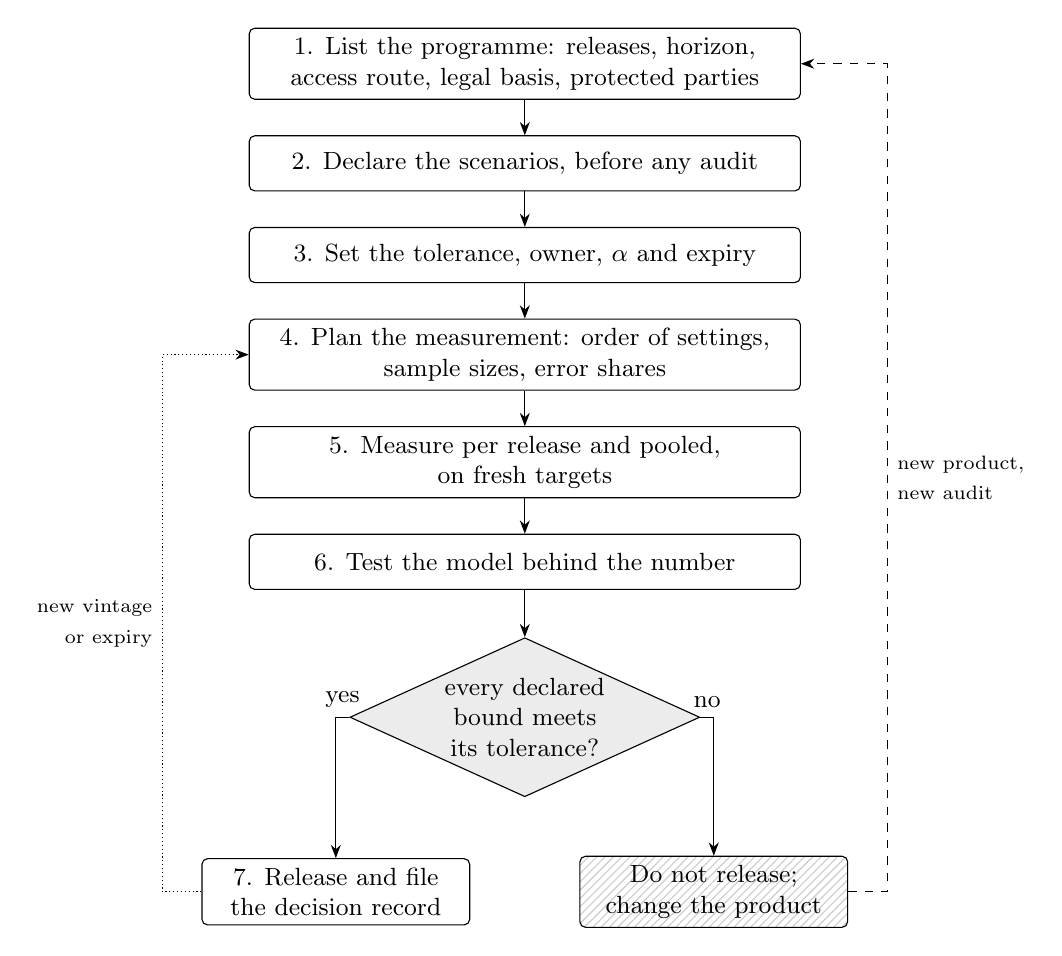
\begin{tikzpicture}[font=\small,node distance=0.45cm,
  stp/.style={draw,rounded corners=2pt,align=center,minimum width=7cm,minimum height=0.7cm},
  gate/.style={draw,diamond,aspect=2.2,align=center,inner sep=1pt,fill=gray!15},
  >=Stealth]
  \node[stp] (s1) {1. List the programme: releases, horizon,\\access route, legal basis, protected parties};
  \node[stp,below=of s1] (s2) {2. Declare the scenarios, before any audit};
  \node[stp,below=of s2] (s3) {3. Set the tolerance, owner, $\alpha$ and expiry};
  \node[stp,below=of s3] (s4) {4. Plan the measurement: order of settings,\\sample sizes, error shares};
  \node[stp,below=of s4] (s5) {5. Measure per release and pooled,\\on fresh targets};
  \node[stp,below=of s5] (s6) {6. Test the model behind the number};
  \node[gate,below=0.6cm of s6] (g) {every declared\\bound meets\\its tolerance?};
  \node[stp,minimum width=3.4cm] (rel) at ($(g.south)+(-2.4,-1.2)$) {7. Release and file\\the decision record};
  \node[stp,minimum width=3.4cm,pattern=north east lines,pattern color=gray!40] (no) at ($(g.south)+(2.4,-1.2)$) {Do not release;\\change the product};
  \draw[->] (s1)--(s2); \draw[->] (s2)--(s3); \draw[->] (s3)--(s4); \draw[->] (s4)--(s5); \draw[->] (s5)--(s6); \draw[->] (s6)--(g);
  \draw[->] (g.west) -| node[near start,above]{yes} (rel.north);
  \draw[->] (g.east) -| node[near start,above]{no} (no.north);
  \draw[->,dashed] (no.east) -- ++(0.5,0) |- node[near start,right,align=left]{\scriptsize new product,\\\scriptsize new audit} (s1.east);
  \draw[->,densely dotted] (rel.west) -- ++(-0.5,0) |- node[near start,left,align=right]{\scriptsize new vintage\\\scriptsize or expiry} (s4.west);
\end{tikzpicture}
\caption{The assessment of a release programme as a decision process. Solid
arrows follow the seven steps of Section~\ref{sec:apply} and Algorithm~\ref{alg:protocol}; the dotted arrow is the
re-assessment at each new vintage or at expiry, which draws on the programme's
remaining error budget; the dashed arrow is a change of product, such as moving
from loan-level files to aggregates or to secure access, which needs a new audit.}
\label{fig:protocol}
\end{figure}

\begin{algorithm}[t]
\caption{Assessing a release programme}\label{alg:protocol}
\begin{algorithmic}[1]
\Require a release programme and the institution's governance record $G$
\State list the releases, horizon, access route, legal basis, protected parties \Comment{Step 1}
\State declare every scenario, pooled ones included, before any audit \Comment{Step 2}
\State set $\tau$ with its owner, harm class, $\alpha$ and expiry \Comment{Step 3}
\State fix the order of settings, the sample sizes and the error shares \Comment{Step 4}
\State measure per release and pooled on fresh targets; choose the setting by
  Algorithm~\ref{alg:selection} or Algorithm~\ref{alg:chain} \Comment{Step 5}
\State run the falsification tests; if one fails, stop: the figure is invalid \Comment{Step 6}
\If{every declared bound meets its tolerance}
  \State release, and file the decision record \Comment{Step 7}
\Else
  \State do not release; change the product and return to Step 1
\EndIf
\State at each new vintage or at expiry, re-assess from Step 4 on the remaining budget
\end{algorithmic}
\end{algorithm}



\paragraph{Step 1. List the programme, not the release.}
Start from the source register, not from the product about to be published. List
every product drawn from it over the planning horizon: monthly or quarterly
aggregates, supervisory publications, research extracts, data shared with other
authorities, and answers to ad hoc requests. For each product record its
frequency, the population it covers, the variables it publishes, and whether any
identifier or stable ordering persists from one vintage to the next. A persistent
pseudonym, a stable row order or a unique combination of rarely changing
attributes lets an adversary match records across vintages, which is the condition that Proposition \ref{prop:nopool} requires. With a persistent pseudonym the products are, for the adversary, one release on the union of their keys (Remark \ref{rem:finer}). Declare a horizon $m$,
the number of vintages the assessment covers. Worksheet 1 records the inventory.

\paragraph{Step 2. Declare the scenarios.}
For each product, and for each combination of products an outsider could hold
together, write down who the adversary is, what it knows, which records it
targets and what harm follows if it succeeds (Section \ref{sec:experiment}). For a
pooled scenario, say whether the adversary knows when the target's record is
present in each vintage, and why (Section \ref{sec:eval-threat}). The
declaration should be specific enough that someone can disagree with it. Table
\ref{tab:apply-map} gives starting declarations for release types common in
central banks. They are illustrations to be adapted, not a statement of what any
institution does. Worksheet 2 records each scenario.

\paragraph{Step 3. Set the tolerance.}
For each harm class the release owner sets a tolerance $\tau$, an error level
$\alpha$, an expiry date and the horizon $m$ of Step 1, and records the legal
basis, the parties the tolerance protects and the access route of the product
(Definition \ref{def:thresh}). The tolerance is the institution's written reading
of when identification is reasonably likely for that adversary and route. Two routes lead to a number. The direct route states the
largest probability of successful exposure the institution will accept for that
harm, taking account of its confidentiality duty and the public value of the
release. The indirect route states the relative weight the institution places on
harm against lost utility and reads the implied tolerance off the risk--utility
frontier (Proposition \ref{prop:tau}, Table \ref{tab:tau}). Either way, the
tolerance is written down before the risk is measured, and a programme tolerance
is set alongside the per-release one. Where the institution has not yet agreed a
tolerance for a harm, the record says so and no decision is made on that harm,
as in the last rows of Table \ref{tab:record}.

\paragraph{Step 4. Plan the measurement.}
Decide how many simulated attacks each scenario needs before running any. With no
observed success, certifying a tolerance $\tau$ at error level $\alpha$ needs
about $\log(1/\alpha)/\tau$ independent attacks, roughly $3/\tau$ at
$\alpha = 0.05$ \citep{hanley1983}; Table \ref{tab:cert} gives exact counts. A
tolerance of $10^{-3}$ needs 2{,}995 attacks, and one of $10^{-5}$ needs
299{,}572, so a very small tolerance can be expensive to certify by simulation.
If the release must pass every one of a fixed set of scenarios or subgroups, each
may be assessed at level $\alpha$, because that is an intersection--union test
(Section \ref{sec:gov}); divide $\alpha$ among them only when their bounds are to
be reported as one simultaneous statement. If a level such as a minimum cell
count is to be chosen from a grid, fix the order in which the levels are tested
before any result is seen (Proposition \ref{prop:fixedseq}). If scenarios may be added after results
are seen, for example because a reviewer proposes a stronger adversary, use a
registered spending sequence rather than a fixed split (Section
\ref{sec:sequential} and the companion article).

\paragraph{Step 5. Measure, per release and pooled.}
Run the declared attacks on the release as it would be published, on fresh
targets, and compute the exact upper bound $\overline{R}_{1-\alpha}$ for each
scenario (Section \ref{sec:est}). Then run the pooled attack over the programme
of Step 1, holding the same auxiliary information, and compute its bound in the
same way (Section \ref{sec:comp}). Report separately any pooled attack that adds
knowledge, such as more readings or the target's history across vintages. The
attacks must be reported side by side. Tables \ref{tab:decomp} and
\ref{tab:robust} show why: on the synthetic register, pooling with one reading
adds nothing unless the adversary knows the loan's history, and part of the
remaining excess comes from the adversary holding more readings, and a committee
needs to know which it is protecting against. Where a level is chosen from a
grid, audit the chosen level again on fresh targets. Report what the chosen
level keeps in volume, such as the share of exposure and of large borrowers, as
well as the share of records.

\paragraph{Step 6. Test the model behind the number.}
Before the bound is used, run the falsification tests of Section
\ref{sec:falsify}: calibration of the linkage posterior, the population-frequency
model, a stronger adversary, monotonicity of the mechanism, the composition test
and temporal transport. A failed test makes the assessment invalid, not failed:
the institution cannot release on it and must repair the model first.

\paragraph{Step 7. Decide, record and re-assess.}
Apply rule \eqref{eq:admiss}: the release passes a scenario only if the upper
bound, not the point estimate, is at or below the tolerance, and it passes
overall only if it passes every declared scenario, pooled ones included. Where
the programme fails, the release fails, even if it passes on its own. File the
decision record (Worksheet 3). Re-assess when the programme is about to pass its
horizon, when a new product is drawn from the same register, when a new public
source could serve as auxiliary information, when the mechanism changes, and at
expiry.

\subsection{Release types common in central banks}\label{sec:apply-map}

Table \ref{tab:apply-map} maps six release types to the objects of Steps 2 to 5.
The first column of the table is the product; the others say whom the adversary
targets, what it plausibly holds, which harm is at stake, which measure of this
paper applies, and where a pooled scenario arises.

\begin{table}[!t]
\centering
\caption{Starting declarations for release types common in central banks. The
entries are illustrations to be adapted to each institution's products, legal
basis and users; they do not describe the practice of any institution.}
\label{tab:apply-map}
\footnotesize
\setlength{\tabcolsep}{3pt}
\begin{tabular}{@{}>{\raggedright\arraybackslash}p{2.3cm}>{\raggedright\arraybackslash}p{2.4cm}>{\raggedright\arraybackslash}p{2.6cm}>{\raggedright\arraybackslash}p{2.3cm}>{\raggedright\arraybackslash}p{2.6cm}>{\raggedright\arraybackslash}p{2.6cm}@{}}
\toprule
Release type & Targets & Adversary holds & Harm & Measure in this paper & Pooled scenario \\
\midrule
Aggregates from a credit register (by sector, region, size) & Borrowers in small cells; lenders in concentrated cells & A firm's sector, region and size from public filings; a lender's own book & Identification of a borrower; a lender's position revealed & Prosecutor risk by cell (Section \ref{sec:three}); residual disclosure from totals (Appendix \ref{app:derivations}) & Monthly vintages; differencing of consecutive months \\
Loan-level research extract & Every borrower in the extract & Key fields and a noisy reading of exposure from other sources & Identification; attribute disclosure of arrears & Linkage attack of Section \ref{sec:eval-threat}; attribute rule & Successive extracts for the same project; extracts for different projects \\
Supervisory statistics by bank group & Individual banks & Each bank's own figures; published annual reports & A bank's confidential figure recovered & Contribution from totals; dominance and $p\%$ rules \citep{hundepool2012} & Quarterly series; tables that share a margin \\
Payment and transaction statistics & Merchants or payers in thin cells & Merchant category and location; own transactions & Identification; commercial information revealed & Prosecutor risk by cell; minimum contributor count & Daily or weekly series of the same cells \\
Household or firm survey microdata & Respondents & Demographic or firm characteristics from registers or social media & Identification; attribute disclosure of wealth or debt & Journalist and marketer measures (Section \ref{sec:three}); frequency model (Section \ref{sec:est}) & Survey waves; the public file and a scientific-use file \\
Answers to ad hoc data requests & Units in the requested breakdown & Everything already published from the same register & Identification by differencing & Differencing posterior (Appendix \ref{app:derivations}) & Each answer pooled with every earlier publication \\
\bottomrule
\end{tabular}
\end{table}

\subsection{When a release fails}\label{sec:apply-fail}

A failed scenario does not end the matter. It tells the committee what to change,
and the record should state which remedy was chosen and why. The remedies fall
into five groups.
\begin{enumerate}
\item \emph{Change the key.} Coarsen the published breakdown, or withdraw the
field that the adversary uses most (Table \ref{tab:ablation} shows how far each
field moves the risk on the synthetic register).
\item \emph{Raise the floor.} Increase the minimum cell count or add a dominance
rule, choosing the level by fixed-sequence testing on the upper bound of the
pooled scenario and confirming it on fresh targets (Table \ref{tab:robust}).
\item \emph{Break the link between vintages.} Rotate pseudonyms, change the row order,
or publish some products less often, so that the pooled adversary cannot match
records across vintages. Rotation is a control on linkability, not
pseudonymisation in the legal sense, and the pseudonym should be a keyed hash
under a key held apart from the release team. It helps only if the published
fields cannot relink the records; on the synthetic credit register the key and
the exact exposure relink every loan, and with exposure rounded to one
significant figure about one loan in ten (Section \ref{sec:eval-programme}).
\item \emph{Add noise.} Use a formal mechanism and account for its budget over the
horizon, remembering that its guarantee bounds posterior odds rather than naming a
linkage probability (Section \ref{sec:dp}).
\item \emph{Change the access route or the product.} Move the product from public
or scientific-use release to a secure research environment, where the risk is
governed by access controls and output checking rather than by the release alone
\citep{desai2016}, or publish aggregates in place of loan-level records. On the
synthetic credit register this is the realistic remedy against an adversary who
knows loan histories, because the floors that meet the tolerance keep a small
share of the exposure (Section \ref{sec:eval-programme}).
\end{enumerate}
Shortening the horizon $m$ is also a remedy, but only if the institution is prepared
to stop the series or re-assess it at the new horizon.

\subsection{Starting small}\label{sec:apply-pilot}

An institution does not need to apply the framework to every product at once. A
workable start is one register and one product family over one quarter:
\begin{enumerate}
\item choose the register whose products are published most often;
\item complete Worksheet 1 for it and agree a horizon;
\item agree one tolerance, for identification, with a named owner;
\item run one per-release and one pooled attack, with the sample sizes of Step 4;
\item file one decision record and present it to the release committee beside the
current method, so the committee can see where the two disagree.
\end{enumerate}
The pipeline that produces this paper runs the attacks and
writes the record. It needs, for each product, the published file or its
specification, the key fields, the auxiliary variables the adversary is declared to
hold and the tolerance. Section \ref{sec:real} shows the demographic path of the
code applied to two public files, which is the pattern for adapting it to an
institution's own data; the credit path has so far run only on the synthetic
register.

\subsection{What the framework does not decide}\label{sec:apply-limits}

The framework makes a decision reproducible; it does not make it for the
institution. It cannot say whether a declared adversary is realistic, whether a
tolerance is legally or ethically right, or whether a release is worth its risk.
Those remain judgements for the release owner. What it adds is that each judgement
is written down, owned and dated, and that the number it is compared with carries
its uncertainty and covers the whole programme.


\section{Worked examples}\label{sec:worked}

The examples below take one step of the method at a time and carry it through
with the numbers of this paper, so that an analyst can reproduce each figure by
hand. Every number comes from the runs reported in Sections \ref{sec:eval} and
\ref{sec:security}, and \nolinkurl{scripts/worked_examples.py} recomputes all of
them into \nolinkurl{artifacts-robustness/worked_examples.json}.
Examples \ref{ex:bound} and \ref{ex:selection} show how a floor is decided,
Example \ref{ex:history} shows the attack that the floor must resist, Examples
\ref{ex:zero} to \ref{ex:length} show how many attacks an audit costs, and
Examples \ref{ex:grinding} and \ref{ex:dp} show what can go wrong and how the
result compares with differential privacy.

\begin{example}[One coordinate, one bound]\label{ex:bound}
Take the single-release attack with one exposure reading at $k_{\min} = 1$, the
first row of Table \ref{tab:robust}. On the confirmation draw the attack named
the right loan for 337 of 4{,}000 targets, a rate of 0.084. Rule \eqref{eq:admiss}
compares the exact one-sided 95 per cent upper bound with the tolerance; that
bound is the 0.95 quantile of the $\mathrm{Beta}(337+1,\,4000-337)$
distribution, which is 0.092. The tolerance is
0.12, so the bound meets it with a margin of $1 - 0.092/0.12 = 0.23$, and the
file passes for this adversary with no suppression. The decision uses the bound,
not the rate: had the rate been 0.115 with the same number of targets, the bound
would have been 0.123 and the release would have failed, as the next example shows.
\end{example}

\begin{example}[Choosing a floor when the confirmation fails]\label{ex:selection}
For the adversary who pools six vintages, holds one reading and knows the
target's history, Algorithm \ref{alg:selection} tests the floors from 300 down on
the selection draw of 4{,}000 targets each. The upper bounds are 0.042 at 300,
0.059 at 200, 0.073 at 150, 0.081 at 100, 0.101 at 75 and 0.111 at 50, all below
0.12, and 0.139 at 40, which fails. The search stops there and selects 50, the
last floor that passed. On the independent confirmation draw the same attack at
50 succeeded for 458 of 4{,}000 targets, a rate of 0.115 with a bound of 0.123,
above the tolerance. The algorithm therefore moves to the next stricter floor,
75, where 384 of 4{,}000 targets were named, a rate of 0.096 with a bound of
0.104, which passes. The floor for this adversary is 75, as Table
\ref{tab:robust} reports. Falling back to 75 keeps the error bound, because 75
had already passed at selection; choosing 40 or 30 after seeing these numbers
would not.
\end{example}

\begin{example}[The history attack on one cell]\label{ex:history}
Consider the four loans of Figure \ref{fig:history}, all in the target's key cell,
with published log exposures 12.0 for the target $t$, 12.7 for $a$, 12.25 for
$b$ and 11.6 for $c$. The adversary's reading of the target is 12.30, with
standard deviation 0.6. Without the history, Algorithm \ref{alg:attack} scores
each loan by the normal density of the reading, and the normalised posteriors are
0.277 for $t$, 0.251 for $a$, 0.313 for $b$ and 0.159 for $c$. The adversary names
$b$, which is wrong, and with a posterior below one half it would not act on the
claim. With the history, $b$ and $c$ are excluded, because $b$ is live in a
vintage where the target is not and $c$ is absent from one where the target is
live. Only $t$ and $a$ remain, with posteriors 0.524 and 0.476. The adversary now
names the target and, with a posterior above one half, acts. Nothing in any
single release changed; the gain comes entirely from the pattern of appearances
across vintages, which is why pooled attacks need coordinates of their own.
\end{example}

\begin{example}[How many attacks certify a coordinate with no successes]\label{ex:zero}
Proposition \ref{prop:cert} gives the fixed-sample count: with no success in $B$
attacks the bound meets $\tau$ when $B \ge \log\alpha/\log(1-\tau)$. At
$\tau = 0.12$ and $\alpha = 0.05$ this is $2.996/0.128 = 23.4$, so 24 attacks. If
the coordinate carries only a third of the error budget, as each attack does when
three are split equally, $\alpha$ becomes $0.05/3$ and the count rises to
$\lceil 4.094/0.128\rceil = 33$. Splitting the budget is therefore cheap when the
risk is far below the tolerance: the count grows with the logarithm of the number
of coordinates, not in proportion to it. The release chain of Algorithm
\ref{alg:chain} avoids even this cost, because a floor that fails ends the search
and each attack keeps the full level.
\end{example}

\begin{example}[The betting gate, draw by draw]\label{ex:gate}
In Algorithm \ref{alg:chain} a coordinate certifies when its evidence $E$ reaches
$1/\alpha = 20$. Fix the bet at $q = 0.05$ with $\tau = 0.12$. Each failed attack
multiplies $E$ by $(1-q)/(1-\tau) = 0.95/0.88 = 1.080$, and each success
multiplies it by $q/\tau = 0.05/0.12 = 0.417$. Starting from $E = 1$, a run of
failures reaches 20 after $\log 20/\log 1.080 = 39.1$ draws, so on the 40th. One
success sets the evidence back by a factor of 0.417, which takes
$\log(1/0.417)/\log 1.080 = 11.4$ further failures to recover. An attack that
succeeds on one target in twenty gains about 0.029 in $\log E$ per draw and so
certifies after about a hundred draws on average, while one that succeeds on one
in nine never gains ground: at
$p = 0.116$ the expected change in $\log E$ per draw is negative for this bet.
The auditor may look at $E$ after every draw and stop at the first crossing
without any correction, which a fixed-sample bound does not allow.
\end{example}

\begin{example}[Why the release chain stops at 150]\label{ex:length}
Near the tolerance the cost of certification is set by the gap between the true
risk and $\tau$. With the best fixed bet, the expected number of draws is about
$\log(1/\alpha)$ divided by the Kullback--Leibler divergence between
$\mathrm{Bernoulli}(p)$ and $\mathrm{Bernoulli}(\tau)$ (the expected-length
proposition of the companion article). For the full pooled attack at
$k_{\min} = 150$, where the true risk is 0.091, that is about 720 draws, well
within the cap of 3{,}000. At $k_{\min} = 100$ the true risk is 0.116, only 0.004
below the tolerance, and the same calculation gives about 43{,}000 draws. The
release chain of Figure \ref{fig:chain} therefore certifies 150 in almost every
stream and 100 only by chance. The floor of 100 is safe, but an audit of any
practical size cannot show it.
\end{example}

\begin{example}[What seed grinding buys an operator]\label{ex:grinding}
Table \ref{tab:audit-process} reports that an honest audit of a coordinate whose
true risk equals the tolerance certifies it falsely in 3.8 per cent of runs. An
operator who can try ten seeds and report the first that passes succeeds with
probability $1 - (1 - 0.038)^{10} = 0.32$, and with a hundred seeds
$1 - (1-0.038)^{100} = 0.98$. The stated error level of 0.05 then means nothing.
Algorithm \ref{alg:committed} removes the choice: the targets are fixed by a
secret committed at registration and by a beacon value published later, so the
operator has one stream per coordinate and the rate returns to 0.038.
\end{example}

\begin{example}[The same tolerance under differential privacy]\label{ex:dp}
Suppose instead that a release were $(\varepsilon,\delta)$-differentially private
with $\varepsilon = 1$ and $\delta = 10^{-6}$, and that a declared attack succeeds
3 per cent of the time when the target's record is replaced by another. The
hypothesis-testing bound of Section \ref{sec:dp} caps that attack's success at
$e^{1}\times 0.03 + 10^{-6} = 0.082$, below the tolerance of 0.12, and the same
cap holds for every attack at once, declared or not. The gate cannot give that
guarantee: its certificate covers the attacks that were registered. What it can
do is certify releases, such as the suppressed loan-level files of this paper,
that have no privacy parameter at all.
\end{example}


\section{What the method adds to the security of a release system}\label{sec:security}

A statistical release system can be assessed in the terms used for any other
information system. This section restates the method in those terms, for readers
in information security, operational risk and internal audit, and follows the
fuller treatment in the companion article. It does not claim that the method
meets, or is certified under, any security standard.

\paragraph{Two adversaries.} The asset is the confidential register: its units
(loans, borrowers and lenders) and their attributes. Disclosure review faces two
adversaries. The first, $\mathcal{A}_{\mathrm{data}}$, holds the releases and the
declared auxiliary information and tries to identify a unit. On the credit
register the record declares three outside classes of it: a single-release
adversary, a pooling adversary with the history, and a pooling adversary with the
history and a reading per vintage (Section \ref{sec:eval-threat}), with the
insider reported beside them. The second, $\mathcal{A}_{\mathrm{op}}$, is whoever
runs the audit and wants a release to pass, through carelessness, deadline
pressure or intent. Per-release review has a model of neither. The method gives a
claim about the first that holds only if the second is contained, so both belong
in the record.

\paragraph{The security claim and what it trusts.} For each declared adversary
and harm class, with probability at least $1-\alpha$, no release is certified
whose declared attack succeeds at a rate at or above the tolerance $\tau$. The
probability is over the simulated attacks, given the register and the declared
attack. It holds for a floor chosen from a grid (Proposition \ref{prop:fixedseq}),
for every subgroup at once (Section \ref{sec:gov}), and while the evidence is
being watched (Proposition \ref{prop:anytime}). It holds against
$\mathcal{A}_{\mathrm{op}}$ only if five things are trusted: (T1) the registry
that stores the audits and the error budget, one per programme and kept across
re-assessments;
(T2) the randomness from which targets are drawn, which the operator cannot
predict when it registers an audit; (T3) the attack code, fixed by a digest when
it is registered; (T4) the list of attacks declared for each release, fixed
before its first outcome; and (T5) a time source the operator does not control.
An operator who chooses the seed knows every outcome in advance, and then no
error statement holds; Example \ref{ex:grinding} puts a number on it.
Figure \ref{fig:trust} draws these boundaries: the outside adversary reads only
the released files, the operator reaches the register only through the registry,
and the five trusted parts sit inside the dashed box. Algorithm \ref{alg:committed}
gives one audit draw under these controls. The bet is written to the ledger before
the target exists, the target is derived from a secret committed at registration
and a beacon value the operator cannot choose, and the outcome is written after
the attack runs, so a later reviewer can recompute every target and check the
order of every entry.

\begin{figure}[t]
\centering
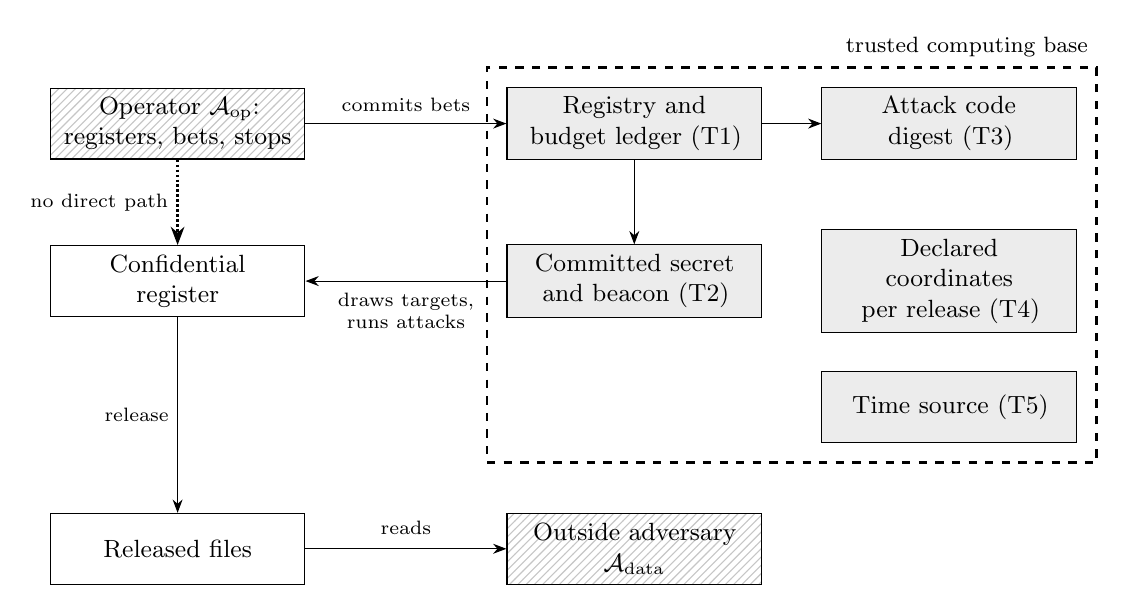
\begin{tikzpicture}[font=\small,
  box/.style={draw,align=center,minimum height=0.9cm,text width=3.0cm},
  tcb/.style={box,fill=gray!15},
  adv/.style={box,pattern=north east lines,pattern color=gray!45},
  lbl/.style={font=\scriptsize,fill=white,inner sep=1pt},
  >=Stealth]
  \node[adv] (op) at (-1.2,0) {Operator $\mathcal A_{\rm op}$:\\registers, bets, stops};
  \node[tcb] (reg) at (4.6,0) {Registry and\\budget ledger (T1)};
  \node[tcb] (code) at (8.6,0) {Attack code\\digest (T3)};
  \node[tcb] (rand) at (4.6,-2.0) {Committed secret\\and beacon (T2)};
  \node[tcb] (decl) at (8.6,-2.0) {Declared\\coordinates\\per release (T4)};
  \node[tcb] (time) at (8.6,-3.6) {Time source (T5)};
  \node[box] (conf) at (-1.2,-2.0) {Confidential\\register};
  \node[box] (rel) at (-1.2,-5.4) {Released files};
  \node[adv] (data) at (4.6,-5.4) {Outside adversary\\$\mathcal A_{\rm data}$};
  \node[draw,dashed,thick,inner sep=7pt,fit=(reg)(rand)(code)(decl)(time)] (tcbbox) {};
  \node[anchor=south east,font=\footnotesize] at (tcbbox.north east) {trusted computing base};
  \draw[->] (op) -- node[lbl,above=3pt]{commits bets} (reg);
  \draw[->] (reg) -- (code);
  \draw[->] (reg) -- (rand);
  \draw[->] (rand) -- node[lbl,below=3pt,align=center]{draws targets,\\runs attacks} (conf);
  \draw[->] (conf) -- node[lbl,left=2pt]{release} (rel);
  \draw[->] (rel) -- node[lbl,above=4pt]{reads} (data);
  \draw[->,densely dotted,thick] (op) -- node[lbl,left=2pt]{no direct path} (conf);
\end{tikzpicture}
\caption{Trust boundaries of the audit. The outside adversary sees only the
released files. The operator reaches the confidential register only through the
registry, which draws targets from committed randomness, records each bet before
the attack runs, runs attack code fixed by its digest and keeps one budget per
programme (Algorithm~\ref{alg:committed}). Everything inside the dashed box must
be trusted for the error bound to hold against the operator; the dotted arrow is
the path that complete mediation forbids. Hatching marks the two adversaries and
grey fill the trusted parts.}
\label{fig:trust}
\end{figure}

\begin{algorithm}[t]
\caption{One committed audit draw}\label{alg:committed}
\begin{algorithmic}[1]
\Require registered coordinate $i$ with commitment $c_i=H(s)$ to an operator secret $s$
  and a beacon round $\beta$ named at registration; draw index $b$; hash-chained ledger $\mathcal L$
\State operator chooses bet $q$ from the ledger alone
\State $\mathcal L.\textsc{append}(\text{bet},i,b,q)$ \Comment{recorded before the target exists}
\State registry checks $H(s)=c_i$ and reads beacon value $\beta$
\State target seed $\gets\mathrm{HMAC}_s(\beta\,\|\,i\,\|\,b)$; draw target $t_{i,b}$ from the registered law
\State run the attack code whose digest was registered; $X\gets$ success on $t_{i,b}$
\State $\mathcal L.\textsc{append}(\text{outcome},i,b,X)$; update $E_{i,b}$ with $(X,q)$
\State publish or time-stamp the ledger head outside the operator's control
\end{algorithmic}
\end{algorithm}



\paragraph{What breaking the trusted parts costs.} Table \ref{tab:audit-process}
measures three ways an operator can break them. An operator who can pick among
seeds, or who runs shadow audits outside the registry and registers only the one
that passed, turns a false-certification rate of 0.038 at the tolerance into
0.322 with ten tries and 0.979 with a hundred, rates computed from the measured
single-try rate with the tries treated as independent. An operator who chooses each bet
of the sequential audit after seeing the outcome certifies an unsafe attack in
every run. The repository implements the matching controls in
\texttt{privacy\_risk.adaptive\_audit}: targets are derived from a committed
secret and a later round of a public randomness beacon, so that neither the
operator nor the beacon alone chooses them; each bet is recorded in a
hash-chained ledger before the attack runs and its outcome is recorded after;
and the ledger's entries cannot be changed, dropped or reordered without breaking
the chain or changing its head. With the controls in place, and the registry
trusted, the rates return to the honest ones.

\begin{table}[t]\centering\small
\caption{Attacks on the audit process. Share of runs in which an unsafe or boundary coordinate is certified, with one coordinate at the full level $\alpha=0.05$ and tolerance 0.12. Seed grinding rows use at most 3{,}000 draws and the capped plug-in bet; post-hoc rows use at most 300 draws and the operator's bet without the control, and the capped plug-in bet with it. Tries is the number of seeds or shadow audits the operator can choose among. Without the control, the rate for several tries is $1-(1-f)^{\rm tries}$ for the single-try rate $f$; with it, the operator has one stream. Script: \nolinkurl{scripts/audit_process_attacks.py}.}\label{tab:audit-process}
\begin{tabular}{lrrrr}
\toprule
Attack on the audit & True risk & Tries & Without control & With control\\\midrule
Seed grinding or shadow audits & 0.12 & 1 & 0.038 & 0.038 \\
Seed grinding or shadow audits & 0.12 & 10 & 0.322 & 0.038 \\
Seed grinding or shadow audits & 0.12 & 100 & 0.979 & 0.038 \\
Seed grinding or shadow audits & 0.14 & 1 & 0.007 & 0.007 \\
Seed grinding or shadow audits & 0.14 & 10 & 0.066 & 0.007 \\
Seed grinding or shadow audits & 0.14 & 100 & 0.495 & 0.007 \\
Bet chosen after the outcome & 0.14 & 1 & 1.000 & 0.007 \\
Bet chosen after the outcome & 0.20 & 1 & 1.000 & 0.000 \\
\bottomrule
\end{tabular}
\end{table}


\paragraph{What it adds over per-release review.} Against
$\mathcal{A}_{\mathrm{data}}$ the method adds four properties.
\begin{enumerate}
\item[(a)] \emph{Programme coverage.} It assesses the pooled, or intersection,
attack over the declared horizon, which Proposition \ref{prop:nopool} shows cannot
be read off per-release figures.
\item[(b)] \emph{Assurance with a stated error.} The decision compares an upper
bound with the tolerance, so the chance of false assurance is at most $\alpha$,
where a point estimate passes a release at the boundary about half the time
(Proposition \ref{prop:point}). Monitoring uses an anytime-valid sequence, so
watching the evidence does not raise the error: in Section
\ref{sec:sequential-evidence}, 20 looks at a fixed-sample bound put it below the
true risk in 21 per cent of runs, against 0 per cent for the anytime sequence.
\item[(c)] \emph{Fail-closed defaults.} These are properties of the pipeline. An
attack that has not been audited is given a risk bound of one and fails, rather
than being treated as zero risk, and the pipeline returns a fail when the upper
bound on the pooled risk of the declared programme exceeds the release
tolerance, even when each release passes on its own (Section \ref{sec:repro}).
\item[(d)] \emph{Red-team findings.} A new attack proposed by a red team enters
as a new coordinate with its own share of the error budget, without voiding the
certificates already issued for earlier coordinates, if budget was reserved for
it, as the companion article shows.
\end{enumerate}
Against $\mathcal{A}_{\mathrm{op}}$ it makes audit shopping, repeating an audit or
scanning settings until one passes, either impossible or paid for out of the
error budget. That holds only under complete mediation \citep{saltzer1975}: every
attack run on the confidential register must pass through the registry, and
development work must use a separate extract. Registering settings, targets,
tolerances and sample sizes before any outcome is seen, and choosing a level by
fixed-sequence testing, are the procedural half of the same condition.

\paragraph{What it does not give.} The implementation is a library, not a
security boundary. Read-only fields in Python are not a security control: code in
the same process can change private state. The SHA-256 hashes a run writes are
the pipeline's manifest of its outputs; they show that a file has changed since
the run, but they carry no key or trusted time stamp, and the ledger's hash chain
detects changes only if its head is published or time-stamped outside the
operator's control. A deployment that must hold against the operator needs the
registry as a separate service with its own storage, signing keys and time
stamps; separation of duties, in which an independent team writes and signs the
attack code, a data custodian holds the register and the randomness commitment,
and the owner signs the tolerance before the first outcome; and verification by
internal audit inside the secure environment, since the log of which targets
were identified is itself confidential. The method gives no guarantee against
attacks that were not registered, and no differential privacy guarantee (Section
\ref{sec:dp}). The evidence in this paper is synthetic, and the floor depends
most on how precisely the adversary can read exposure (Table
\ref{tab:replication}), which an institution has to argue for from what it knows
of the sources outsiders hold.

\paragraph{Relation to security-assessment practice.} The declared scenario is a
threat model in the usual sense \citep{shostack2014}: asset, adversary, capability
and harm are written down before testing. The attack simulation is red-team
testing with a statistical stopping rule. The decision record is an assurance
case: a claim (the release meets $\tau$ against the declared adversaries), the
evidence (bounds, sample sizes and falsification tests) and the argument that
links them (the propositions of this paper), with a named owner and an expiry
date. The mapping is offered to help an institution place the method within its
existing risk and audit processes, not as a claim of conformity with any
standard.

\section{Discussion}\label{sec:disc}

The argument of this paper is that a release decision has three parts that
should be separately visible, and that most of the difficulty in practice comes
from collapsing them. Section \ref{sec:experiment} shows that the standard risk
measures are theorems about one linkage experiment, so that changing the
experiment changes the measure; Section \ref{sec:est} shows that the resulting
figure is an estimate whose uncertainty belongs in the decision rule; Section
\ref{sec:gov} shows that the tolerance is a policy quantity that a stated relative harm weight
already pins down. Two negative results follow. The first holds by
construction: a $k$-anonymous release does not guarantee a risk of $1/k$ once the
adversary holds a variable the key leaves out (Table \ref{tab:kanon}), and its use
is to show how large the gap can be, not to reveal a flaw in the criterion. The
second has more consequence for institutions: when records carry a persistent
pseudonym, a programme of low-risk releases can be attacked far above the bound
its marginals imply (Table \ref{tab:comp}). Section \ref{sec:eval} shows what the
second costs on a release system rather than in a construction, and what it
depends on. On the synthetic register, with the floor chosen by fixed-sequence
testing and confirmed on fresh targets, per-release review passes the file with
no suppression, or with a floor of 20 when every size class must pass. An
adversary who pools the vintages and knows when the target's loan is live needs
75 (200 for every size class); without that knowledge pooling adds nothing there.
An adversary that also holds a reading per vintage needs 150, and no floor up to
200 protects every size class. An insider who reads exposure closely is stopped
by no floor. The answers are all correct, for different adversaries, and the
choice among them is the institution's declaration, not a result of the analysis
(Table \ref{tab:robust}).

The cost is the finding a committee should weigh most. The floor of 150 keeps 20
per cent of loans and 4 per cent of exposure, and no loan to a large firm, so the
file that survives is not the file that concentration and supervisory analysis
need. We draw a plain conclusion from this for the synthetic register: against an
adversary who knows loan histories, a loan-level release is the wrong product.
The realistic options are aggregates with contributor and count rules, or access
to the loan-level file in a secure setting, where the Five Safes govern who sees
it and what leaves. The loan-level file here stands in for securitisation
loan-level disclosures and for research files as an accredited user sees them;
it is not a claim that any central bank publishes loan-level credit data.

Four limitations apply. First, the simulation is synthetic.
It establishes that the phenomena occur under a transparent data generating
process and that the estimators behave as the propositions say, and it cannot
establish the magnitudes an agency would see on its own register; those depend
on the auxiliary data actually available, which is exactly the quantity a
declared scenario has to guess. Second, the framework represents harm through a
scalar $c_h$ within a declared class $h$. Harms that fall on groups rather than
individuals, and harms that arise from correct inference about a population
rather than identification of a person, are outside it, and the second of these
is precisely what \citet{dwork2014} argue is not a privacy violation at all.
Third, the joint attacks are one pooling rule among many, and they assume a
record identifier shared across releases. They measure what pooling achieves for
that adversary's information, so they support the negative result of
Proposition \ref{prop:nopool}, but no simulation can deliver the supremum over
rules that a formal guarantee delivers by construction. Fourth, the credit
floors are conditional. They depend on the tolerance (Table
\ref{tab:tolerance-floors}), on the precision of the adversary's exposure reading
(Table \ref{tab:replication}), which an institution can argue for but not
measure, and on a register whose exposures do not change between vintages.

Four extensions look tractable. The frontier estimation in Section
\ref{sec:ru} could be given a proper inferential treatment, since the frontier is a functional of an estimated set and its selected point
is biased in the same way as any quantity chosen by maximising an estimate. The risk budget of Proposition
\ref{prop:budget} could be extended from the union event to a joint accountant
that admits dependence, which would need a composition theorem for
scenario-conditional risk under a stated dependence class. The implied tolerance
of Proposition \ref{prop:tau} could be estimated from revealed institutional
behaviour, since agencies have been making these decisions for decades and
their past choices identify $\kappa$ under the framework. And the calibration
test of Section \ref{sec:falsify} could be developed into a formal
specification test with a distribution under the null.

The recommendation is to publish, alongside each release decision, the risk
estimate, the uncertainty bound and the number of replicates behind it, the
tolerance, the adversary specification, the legal basis and access route, the
mechanism setting with what it keeps in records and in volume, the named owner
and the expiry date. For a programme, publish the joint simulation and its
horizon as well. The record does not remove judgement from the decision. It
places the judgement in the tolerance and leaves the probability calculation
reproducible and open to being proved wrong.

\subsection{What a release committee should take from this}

Three decisions follow from the argument, and each needs a committee. The first is the tolerance, its accountable owner and its expiry date,
which Definition \ref{def:thresh} makes a record rather than a habit. Section \ref{sec:apply} sets out how to reach it. The
second is whether that tolerance is asserted of each release or of the programme,
which Section \ref{sec:eval} shows is not a matter of wording: on the synthetic
register, at a tolerance of 0.12, the per-release reading of the rule releases all
27{,}167 loans of the first vintage, while the programme reading against the full
adversary releases 5{,}553, with 4 per cent of the exposure. The third is the
adversary specification, written down, so that the assumption can be disagreed
with explicitly instead of inherited silently. On the credit register it decides
the floor: whether the adversary knows the history of the target's loan moves the
programme floor from 1 to 75, and whether it holds a reading in every vintage
moves it from 75 to 150.

A fourth choice is easy to miss because the arithmetic hides it. The measures of
Section \ref{sec:three} protect different people. The marketer measure is an
average over the released records, and a release can meet a tolerance on that
average while a particular record in it is identified with near certainty. The
prosecutor measure in its supremum form protects the most exposed record instead,
and the subgroup bounds of Section \ref{sec:eval} are the operational form of
the same idea. Which one an institution reports is an ethical choice about whose
protection the threshold is for, not a technical preference, and the framework
supports either as long as the committee says which it has chosen.

\section{Conclusion}\label{sec:conclusion}

A release programme, not a release, is the object a central bank should govern.
When records keep a pseudonym across vintages, per-release risk figures cannot
bound what an adversary who holds every vintage can do, and a point estimate at
the tolerance passes about half the time. The rule we propose compares an exact
upper bound on the programme's risk with a written tolerance that has an owner,
an expiry date, a harm class, a horizon, a legal basis and an access route, and
it chooses the protection level by fixed-sequence testing, confirmed on fresh
targets, with the adversary set declared before any table is read.

On a synthetic credit register at a tolerance of 0.12, that rule passes the
loan-level file with no suppression on one release, needs a floor of 75 against
an adversary who knows loan histories and 150 against one who also reads
exposure in each vintage, and finds no floor against an insider. The floor of
150 keeps a fifth of the loans and 4 per cent of the exposure, and no large firm.
The floors move with the tolerance and with the adversary's reading precision,
so both belong in the record. For a register like this one, and an adversary who
knows loan histories, the loan-level file is the wrong product: aggregates, or
access in a secure setting, are the options a committee can defend. The results
are synthetic, and the pipeline that produced them can be run on a real register
inside the institution that holds it.

\subsection*{Data and code availability}

The pipeline in the companion repository generates every table, figure and quoted
study result, and writes the configuration and recorded outputs to
\nolinkurl{artifacts-paper/}. The script \nolinkurl{scripts/check_paper_numbers.py}
checks the figures quoted in the prose against the run. The script
\nolinkurl{scripts/programme_robustness.py} writes
\nolinkurl{artifacts-robustness/robustness.json}, the source of Tables
\ref{tab:robust}, \ref{tab:tolerance-floors} and \ref{tab:replication}, and
\nolinkurl{scripts/estimand_check.py} writes
\nolinkurl{artifacts-robustness/estimand_check.json}. The module
\texttt{privacy\_risk.adaptive\_audit} implements the audit-process controls of
Section \ref{sec:security}, and \nolinkurl{scripts/audit_process_attacks.py}
produces Table \ref{tab:audit-process}. The neural release pipeline of Section
\ref{sec:eval-neural} is \texttt{privacy\_risk.neural\_pipeline}, which writes
\nolinkurl{artifacts-neural/neural_pipeline.json} and Table
\ref{tab:neural-pipeline}. The earlier procedure of the online appendix is
\texttt{privacy\_risk.neural\_trust} and supplies no inputs to the tables or
figures here. The two public microdata files
of Section \ref{sec:real} are loaded through the \texttt{wooldridge} package.

\subsection*{Acknowledgements}

An earlier version was prepared for the Workshop on Data Security and Privacy of
the Banco de Portugal and the Irving Fisher Committee, Lisbon, September 2026.
The views are the author's own.

\appendix
\addtocontents{toc}{\protect\medskip\noindent\textbf{Appendices}\par}

\section{Allocating a programme tolerance}\label{app:budget}

Suppose an institution governs the union event, so that the programme
constraint is $\sum_i R_i \leq \tau_{\mathrm{prog}}$ by \eqref{eq:boole}. This is
not a conservative route: by Proposition \ref{prop:nopool} the pooled risk can
exceed the union bound. Each release has value weight $w_i > 0$ and frontier
$\varphi$ shared across releases for simplicity.

\begin{proposition}[Risk budget]\label{prop:budget}
The problem $\max \sum_i w_i \varphi(r_i)$ subject to $\sum_i r_i \leq
\tau_{\mathrm{prog}}$ and $r_i \geq 0$, with $\varphi$ increasing,
differentiable and strictly concave, and with $\varphi'(0^+) = \infty$, so that no release is
allocated zero risk, has a unique solution characterised by
\begin{equation}
w_i \varphi'(r_i^\star) = \mu \quad \text{for all } i, \qquad
\sum_i r_i^\star = \tau_{\mathrm{prog}} ,
\label{eq:water}
\end{equation}
for a multiplier $\mu > 0$. If $\varphi(r) = \log r$ then $r_i^\star =
\tau_{\mathrm{prog}} w_i / \sum_j w_j$, so the budget is allocated in
proportion to value.
\end{proposition}

\begin{proof}
See Appendix \ref{app:proofs}.
\end{proof}

The equal split $r_i = \tau_{\mathrm{prog}}/m$, which is what an institution
does by default when it applies one tolerance to every release, satisfies
\eqref{eq:water} only if all $w_i$ are equal. The proportional rule is equally
particular: it holds for the logarithmic value curve and for no other. For the
power family $\varphi(r) = a + b r^{\gamma}$ with $b < 0$ and $\gamma < 0$,
which is the family that fits the simulated frontier, condition
\eqref{eq:water} gives
\begin{equation}
r_i^\star \ \propto \ w_i^{1/(1-\gamma)} ,
\label{eq:power}
\end{equation}
so the allocation is flatter than value whenever $\gamma < 0$, and it
approaches an equal split as $\gamma \to -\infty$. In the simulation the fitted $\gamma = -0.23$ gives an exponent of 0.81, and
on the fitted curve the resulting allocation cuts the total loss by 4.5 per cent
relative to the equal split. That figure is a stylised illustration: the
attainable frontier is not concave, and the curve smooths it (Section
\ref{sec:sim}).

We stress the scope. Proposition \ref{prop:budget} governs the union event. It
does not govern the pooled attack, and by Proposition \ref{prop:nopool} nothing
stated in terms of the marginals can. A risk budget is a device for allocating
attention across releases, not a substitute for joint simulation.

\section{Proofs}\label{app:proofs}

\begin{proof}[Proof of Proposition \ref{prop:recip}]
Condition on $S_t = 1$ and $K_a(X_t) = k$. By Assumption \ref{as:key} the
released key of every record equals its confidential key, and by Assumption
\ref{as:obs} the adversary observes $k$. The compatible set is therefore
$\{j \in I : K_a(X_j) = k\}$, which has cardinality $f_k$ by \eqref{eq:freq}
and contains $t$. By Assumption \ref{as:exch} the adversary's information is
invariant to permutations of that set, and by Assumption \ref{as:unif} it
selects each member with probability $1/f_k$. Exactly one member is correct,
so
\[
\Prob\{\delta_a = t \mid S_t = 1, K_a(X_t) = k, f_k\}
= \sum_{j=1}^{f_k} \frac{1}{f_k}\ind{j = t} = \frac{1}{f_k} . \qedhere
\]
\end{proof}

\begin{proof}[Proof of Proposition \ref{prop:kanon}]
By \eqref{eq:pros} and Proposition \ref{prop:recip}, $\sup_{t \in I}
R_{\mathrm{pros}}(t,\theta) = 1/\min_{k : f_k > 0} f_k$. Hence $\sup_t
R_{\mathrm{pros}} \leq \tau$ if and only if $\min_k f_k \geq 1/\tau$, and since
$f_k$ is an integer this is $\min_k f_k \geq \lceil 1/\tau \rceil$, which is the
definition of $k$-anonymity with $k = \lceil 1/\tau\rceil$.

For the failure claim, drop Assumption \ref{as:exch}. Let the release publish a confidential
variable $y$ alongside the key, let a key class have $f_k = k$ members with
distinct values of $y$, and let the adversary observe $z_t = y_t + \sigma \xi$ with $\xi$ standard normal and
$\sigma$ small relative to the within-class spacing of $y$. The posterior
\eqref{eq:post} concentrates on the member whose $y$ is nearest $z_t$, and as
$\sigma \downarrow 0$ the success probability of the maximum-posterior rule
tends to one, while $k$-anonymity holds for every $\sigma$. Therefore
$\sup_t R_a^{\mathrm{in}} > 1/k$ for all sufficiently small $\sigma$.
\end{proof}

\begin{proof}[Proof of Proposition \ref{prop:cert}]
With zero successes the one-sided Clopper--Pearson upper limit solves $(1 -
U)^B = \alpha$, giving $\overline{R}_{1-\alpha} = 1 - \alpha^{1/B}$ as in \eqref{eq:cp0}.
Then $\overline{R}_{1-\alpha} \leq \tau$ if and only if $\alpha^{1/B} \geq 1 - \tau$.
Taking logarithms, and noting $\log \alpha < 0$ and $\log(1-\tau) < 0$, this is
$B^{-1}\log\alpha \geq \log(1-\tau)$, that is $B \geq \log\alpha /
\log(1-\tau)$. Since $\log(1-\tau) = -\tau + O(\tau^2)$, the right side is
$-\log\alpha/\tau + O(1)$ as $\tau \downarrow 0$.
\end{proof}

\begin{proof}[Proof of Proposition \ref{prop:plugin}]
For any occupied key class, $f_k \leq F_k$ by \eqref{eq:freq}, hence $1/f_k
\geq 1/F_k$ pointwise, and monotonicity of expectation gives the first claim,
with equality if and only if $f_k = F_k$ almost surely for every class the
average touches. The second claim is Jensen's inequality applied to the convex
function $x \mapsto 1/x$ on $(0, \infty)$, which is strict unless $f_k$ is
degenerate.
\end{proof}

\begin{proof}[Proof of Proposition \ref{prop:point}]
At $R_a = \tau$, asymptotic symmetry of the estimator gives
$\Prob(\widehat{R}_a \leq R_a) \to 1/2$, so the point-estimate rule releases
with probability tending to $1/2$. A valid one-sided $(1-\alpha)$ upper bound
satisfies $\Prob\{R_a \leq \overline{R}_{1-\alpha}\} \geq 1 - \alpha$, hence
$\Prob\{\overline{R}_{1-\alpha} < R_a\} \leq \alpha$. At the boundary, release under
\eqref{eq:admiss} implies $\overline{R}_{1-\alpha} \leq \tau = R_a$, an event of
probability at most $\alpha$ up to equality conventions.
\end{proof}

\begin{proof}[Proof of Proposition \ref{prop:fixedseq}]
Write $H_i$ for the hypothesis that $R(\theta_i) > \tau$, and say that setting
$i$ passes when its bound is at or below $\tau$. If every $H_i$ is false there is
nothing to prove. Otherwise let $i^\ast$ be the first index in the fixed order for
which $H_{i^\ast}$ is true. The procedure chooses a setting $j$ only if settings
$1, \dots, j$ all pass, so it chooses a setting with true risk above $\tau$ only
if it chooses some $j \geq i^\ast$, which requires that setting $i^\ast$ pass.
Setting $i^\ast$ is fixed before the data are seen, so by the one-sided bound at
level $\alpha$ the probability that it passes while $R(\theta_{i^\ast}) > \tau$
is at most $\alpha$. Hence the probability of choosing an unsafe setting is at
most $\alpha$. No step uses the order of the true risks, so the result holds
whether or not they are monotone \citep{maurer1995}.
\end{proof}

\begin{proof}[Proof of Proposition \ref{prop:tau}]
On the frontier the problem is $\max_r \{\lambda\varphi(r) - c_h r\}$ over
$[\underline r, \overline r]$. The objective is strictly concave because
$\varphi$ is, so a maximiser exists and is unique. Its derivative is
$\lambda\varphi'(r) - c_h$, which is strictly decreasing; under
$\varphi'(\underline r) > \kappa > \varphi'(\overline r)$ with $\kappa = c_h /
\lambda$ it is positive at $\underline r$ and negative at $\overline r$, so the
maximiser is interior and solves $\varphi'(r) = \kappa$. Monotonicity of
$\tau^\star$ in $\kappa$ follows because $\varphi'$ is strictly decreasing, so
$\tau^\star = (\varphi')^{-1}(\kappa)$ is decreasing in $\kappa$.
\end{proof}

\begin{proof}[Proof of Proposition \ref{prop:exist}]
The feasible set $\Theta_\tau = \{\theta : \sup_{t}\overline{R}_{1-\alpha}(t,\theta) \leq
\tau\}$ is closed by lower semicontinuity of the constraint function, hence
compact as a closed subset of the compact $\Theta$, and nonempty by assumption.
An upper semicontinuous function attains its maximum on a nonempty compact set.
\end{proof}

\begin{proof}[Proof of Proposition \ref{prop:boole}]
Monotonicity gives $C_i \subseteq \bigcup_j C_j$ and hence $R_i \leq R_\cup$
for every $i$, so $\max_i R_i \leq R_\cup$. Boole's inequality gives $R_\cup
\leq \sum_i R_i$, and $R_\cup \leq 1$ always, which is the upper bound.
Attainment: if the events are nested, $C_1 \supseteq C_2 \supseteq \cdots$,
then $R_\cup = R_1 = \max_i R_i$. If they are disjoint and $\sum_i R_i \leq 1$,
then $R_\cup = \sum_i R_i$; if $\sum_i R_i > 1$, a standard overlapping
construction on $[0,1]$ with Lebesgue measure, placing $C_i$ as intervals that
cover $[0,1]$, gives $R_\cup = 1$.
\end{proof}

\begin{proof}[Proof of Proposition \ref{prop:nopool}]
Fix $m \geq 2$ and an integer $k \geq 1/\nu$. Let the sample consist of
$n = k^m$ units labelled by the vectors $x = (x_1, \dots, x_m) \in \{1, \dots,
k\}^m$, all present with certainty. Let release $i$ publish the key
$K_i(x) = (x_1, \dots, x_{i-1}, x_{i+1}, \dots, x_m)$, that is all coordinates
except the $i$th. Each key class of release $i$ contains exactly $k$ units, so
the release is $k$-anonymous and, under Assumptions \ref{as:key} to
\ref{as:unif}, $R_i = 1/k \leq \nu$.

Now let the adversary hold all $m$ releases and know the target's full label.
The candidate set from release $i$ is $\{x : K_i(x) = K_i(t)\}$, which is the
set of units agreeing with $t$ in all coordinates except possibly the $i$th.
The intersection over $i = 1, \dots, m$ of these sets is $\{t\}$, because a
unit in the intersection agrees with $t$ in every coordinate: for coordinate
$j$, membership in the candidate set of any release $i \neq j$ forces
$x_j = t_j$, and $m \geq 2$ guarantees such an $i$ exists. Hence
$\delta_a^{(m)}$ that selects the unique element of the intersection satisfies
$R_{\mathrm{pool}} = 1$. Since $\nu$ was arbitrary and
$(R_1, \dots, R_m) = (1/k, \dots, 1/k)$ can be made arbitrarily small while
$R_{\mathrm{pool}} = 1$, no function of the marginals can bound
$R_{\mathrm{pool}}$ from above.

For the final claim, let $A_i(t)$ be the candidate set of release $i$ and
$G_m(t) = \bigcap_{i \leq m} A_i(t)$, and suppose the adversary selects
uniformly from $G_m(t)$. Then $G_{m+1}(t) \subseteq G_m(t)$ and $t \in G_m(t)$
for every $m$, so $1/|G_{m+1}(t)| \geq 1/|G_m(t)|$ pathwise and taking
expectations gives monotonicity. Since $G_m(t) \subseteq A_i(t)$ for each
$i \leq m$, the same argument gives $R_{\mathrm{pool}} \geq \max_{i \leq m}
\E[1/|A_i(t)|] = \max_i R_i$.
\end{proof}

\begin{proof}[Proof of Proposition \ref{prop:budget}]
The objective is strictly concave and the constraint set is compact and convex,
so a unique maximiser exists. Since $\varphi$ is increasing, the constraint
binds. The Lagrangian is $\sum_i w_i\varphi(r_i) - \mu(\sum_i r_i -
\tau_{\mathrm{prog}})$ and the first-order conditions are $w_i\varphi'(r_i) =
\mu$ for every $i$, which is \eqref{eq:water}; concavity makes them sufficient.
For $\varphi = \log$ the conditions read $w_i / r_i = \mu$, so $r_i \propto
w_i$, and the constraint fixes the constant at $\tau_{\mathrm{prog}}/\sum_j
w_j$. For $\varphi(r) = a + b r^{\gamma}$ with $b < 0$ and $\gamma < 0$, which
is increasing and strictly concave on $(0,\infty)$, we have $\varphi'(r) = b
\gamma r^{\gamma - 1}$, so \eqref{eq:water} reads $w_i r_i^{\gamma - 1} =
\mu / (b\gamma)$ and hence $r_i \propto w_i^{1/(1-\gamma)}$, which is
\eqref{eq:power}.
\end{proof}

\begin{proof}[Proof of Proposition \ref{prop:attack-threshold}]
At posterior probability $p$, acting has expected payoff
$V(p)=ph-(1-p)c_f-c_a=p(h+c_f)-(c_f+c_a)$, which is increasing in $p$
because $h+c_f>0$. Its largest value is $V(1)=h-c_a$. If $c_a>h$ then
$V(p)<0$ for every $p\le1$, and if $c_a=h$ then $V(p)\le0$ with equality only at
certainty, where acting gains nothing; in both cases the adversary does not act,
which we record as $p^\star=+\infty$. If $c_a<h$, then $V(p)\ge0$ if and only if
$p\ge(c_f+c_a)/(h+c_f)$, and this ratio is below one because $c_f+c_a<h+c_f$.
Finally $(c_f+c_a)/(h+c_f)=1/2$ if and only if $2c_f+2c_a=h+c_f$, that is
$h=c_f+2c_a$.
\end{proof}

\begin{proof}[Proof of Proposition \ref{prop:anytime}]
For fixed $u\in(0,1)$, the Bernoulli likelihood ratio through time $B$ between
risk $u$ and risk $r_0$ is a nonnegative $r_0$-martingale with initial value
one. Integrating these likelihood-ratio martingales against the
$\mathrm{Beta}(a,b)$ density preserves the martingale property by Tonelli's
theorem and gives exactly \eqref{eq:eprocess}. Ville's inequality for a
nonnegative martingale yields \eqref{eq:ville}. The event that $r_0$ exits
$\mathcal C_B$ at some time is the event that $E_B(r_0)\ge1/\alpha$ at some
time, so its probability is at most $\alpha$.
\end{proof}

\begin{proof}[Proof of Proposition \ref{prop:dpbound}]
Let $x$ and $x'$ be the databases in which $H$ is true and false respectively;
they differ in one individual's record, so they are neighbouring, and by
hypothesis the remaining records have the same distribution under both. For any
observed output set $E$ of positive probability, \eqref{eq:dp} with
$\delta_{\mathrm{dp}} = 0$ gives the likelihood ratio bound
$\Prob\{M(x) \in E\} / \Prob\{M(x') \in E\} \leq e^\varepsilon$. Bayes' rule in odds form gives
\[
\frac{\Prob(H \mid M \in E)}{1 - \Prob(H \mid M \in E)}
= \frac{p}{1-p}\cdot\frac{\Prob\{M(x) \in E\}}{\Prob\{M(x') \in E\}}
\leq \frac{p}{1-p}e^{\varepsilon} ,
\]
and solving for $\Prob(H \mid M \in E)$ gives \eqref{eq:dppost}. With
$\delta_{\mathrm{dp}} > 0$ the same steps give the exact bound
\[
\frac{\Prob(H \mid M \in E)}{1 - \Prob(H \mid M \in E)}
\leq \frac{p}{1-p}\Bigl(e^{\varepsilon}
+ \frac{\delta_{\mathrm{dp}}}{\Prob\{M(x') \in E\}}\Bigr) ,
\]
which is unbounded for rare $E$, so no uniform posterior bound holds when
$\delta_{\mathrm{dp}} > 0$. With probability at least
$1 - O(\delta_{\mathrm{dp}}/(1-e^{-\varepsilon}))$ over outputs, a bound of the
form \eqref{eq:dppost} holds with $\varepsilon$ inflated by a constant factor
\citep{kasiviswanathan2014}.
\end{proof}

\section{Expanded derivations}\label{app:derivations}

This appendix expands the calculations used in the text, so that each reported
quantity can be reconstructed without treating an intermediate identity as
given.

\subsection{From joint success to membership-conditional risk}

Let $A_t=\{\delta_a(Z_t,Y_\theta)=t\}$ and $B_t=\{S_t=1\}$. Since a released
record cannot equal an unsampled target, $A_t\subseteq B_t$, and
\begin{equation}
R_a^{\mathrm{unc}}(t,\theta)
 =\Prob(A_t\cap B_t\mid\mathcal{B}_a)
 =\Prob(A_t\mid B_t,\mathcal{B}_a)\Prob(B_t\mid\mathcal{B}_a)
 =\pi_t R_a^{\mathrm{in}}(t,\theta),
\end{equation}
which is \eqref{eq:factor}. If the auxiliary information changes the adversary's
belief about membership, the last factor is $\Prob(B_t\mid\mathcal{B}_a)$ and not
the design probability $\pi_t$; using $\pi_t$ requires that $\mathcal{B}_a$ carry
no information about who was sampled.

\subsection{Bayesian linkage from comparison vectors}

Let $\gamma_{tj}=\gamma(Z_t,Y_j)$ be a comparison vector, and write
$m(\gamma)=p(\gamma\mid H_{tj}=1)$ and $u(\gamma)=p(\gamma\mid H_{tj}=0)$ for its
density under a match and a non-match, with likelihood ratio
$\Lambda_{tj}=m(\gamma_{tj})/u(\gamma_{tj})$. Under the usual assumptions that the fields of a comparison vector are
conditionally independent given the match status \citep{fellegi1969}, and that the
comparison vectors of distinct candidates are conditionally independent of one
another, Bayes' theorem and division by $\prod_\ell u(\gamma_{t\ell})$ give
\begin{equation}
p_{tj}=\frac{q_{tj}\Lambda_{tj}}
 {q_{t0}\Lambda_{t0}+\sum_{\ell\in I}q_{t\ell}\Lambda_{t\ell}},
\end{equation}
where $\Lambda_{t0}=1$, because under the no-match hypothesis every candidate is
scored by its non-match density and the division leaves one. This is
\eqref{eq:post} with $L=\Lambda$. Exact exchangeable matching is the case
of equal likelihood and prior weight on each of the $f_k$ compatible records and
zero weight elsewhere, giving $1/f_k$ for each. For two candidates,
\begin{equation}
\frac{p_{tj}}{p_{t\ell}}
=\frac{q_{tj}}{q_{t\ell}}\cdot\frac{L_{tj}}{L_{t\ell}} ,
\label{eq:posterior-odds-link}
\end{equation}
so the reciprocal-frequency figure is valid only when both ratios equal one inside
the key class. Equation \eqref{eq:posterior-odds-link} is where informative side
information enters.

\subsection{The uniqueness probability under binomial thinning}

Conditional on $F_k=v$, Bernoulli sampling gives $f_k\mid F_k=v\sim
\mathrm{Binomial}(v,\pi)$, so $\Prob(F_k=1,f_k=1)=\pi\Prob(F_k=1)$ and
$\Prob(f_k=1)=\sum_{v\ge1}v\pi(1-\pi)^{v-1}\Prob(F_k=v)$. Dividing the first by
the second gives \eqref{eq:rho}. For a parametric frequency law $g(v;\eta)$ the
plug-in estimator is
\begin{equation}
\widehat\rho_k=
\frac{\pi g(1;\widehat\eta)}
 {\sum_{v\ge1}v\pi(1-\pi)^{v-1}g(v;\widehat\eta)} ,
\end{equation}
and the analyst must carry the uncertainty in $\widehat\eta$ through
\eqref{eq:delta-risk}, or refit $g$ inside each replicate.

\subsection{Exact binomial bounds and simultaneous control}

If $X=\sum_b C_t^{(b)}=x$, the one-sided Clopper--Pearson upper endpoint is
\begin{equation}
\overline{R}_{1-\alpha}(x,B)=
\mathrm{Beta}^{-1}_{1-\alpha}(x+1,B-x),\qquad x<B,
\label{eq:cp-general}
\end{equation}
and one when $x=B$, where $\mathrm{Beta}^{-1}_q(a,b)$ is the $q$th quantile of a
beta distribution. At $x=0$ the beta distribution function is $F(u)=1-(1-u)^B$,
so $F(\overline{R})=1-\alpha$ recovers \eqref{eq:cp0}.

If $T$ holds $q$ targets and the decision uses their maximum, separately valid
$(1-\alpha)$ intervals do not give a $(1-\alpha)$ file-level statement. Bonferroni control uses targetwise error $\alpha/q$. Section \ref{sec:kanon} needs
the lower form, since it reports the worst target, so writing
$\underline{R}_{\alpha/q,t}$ for a one-sided lower limit,
\begin{equation}
\Prob\left\{R_t\ge \underline{R}_{\alpha/q,t}\ \text{for every }t\in T\right\}
\ge 1-\sum_{t\in T}\frac{\alpha}{q}=1-\alpha ,
\label{eq:bonf}
\end{equation}
and the same argument gives the upper form when every target's bound is to be
reported at once. This is conservative but valid without independence, and it is
what Section \ref{sec:kanon} uses for the worst target. A release decision that
requires every target's bound to meet $\tau$ does not need it: that is an
intersection--union test, and per-target bounds at level $\alpha$ already
control false release at $\alpha$ \citep{berger1982}. A max-statistic bootstrap can replace
it when the resampling scheme preserves dependence across targets
\citep{efron1993}.

\subsection{Three layers of uncertainty}

It is useful to separate three layers of uncertainty that are otherwise hidden
inside one error bar. Write $\widehat\eta$ for parameters estimated from an
auxiliary source and $\mathcal{D}$ for the realised confidential sample. The law
of total variance gives
\begin{equation}
\mathrm{Var}(\widehat R_a)
=\E_{\mathcal{D},\widehat\eta}
  \{\mathrm{Var}(\widehat R_a\mid\mathcal{D},\widehat\eta)\}
 +\mathrm{Var}_{\mathcal{D},\widehat\eta}
  \{\E(\widehat R_a\mid\mathcal{D},\widehat\eta)\}
= V_{\mathrm{MC}} + V_{\mathrm{input}} ,
\label{eq:var-decomp}
\end{equation}
where the second term collects everything that varies with the sample and the
fitted inputs rather than with the simulation. A nested design that redraws the sample estimates the part of it that the sampling
design contributes. Separating that from the contribution of a refitted auxiliary
model needs a second level of nesting, and the two parts do not in general add,
because the risk is not separable in the two inputs.
The binomial expression in \eqref{eq:mc} estimates only $V_{\mathrm{MC}}$.
Increasing $B$ drives that term to zero and does nothing to the others.

For a smooth risk functional $R(\eta)$ with $\sqrt m(\widehat\eta-\eta_0)
\Rightarrow N(0,\Sigma_\eta)$, the delta method supplies the first-order
approximation \citep{vandervaart1998}
\begin{equation}
\mathrm{Var}_{\mathrm{aux}}\{R(\widehat\eta)\}
\approx \frac{1}{m}\nabla_\eta R(\eta_0)^\top
\Sigma_\eta\nabla_\eta R(\eta_0) .
\label{eq:delta-risk}
\end{equation}
Non-smooth operations such as a maximum over targets invalidate this calculation
at ties, and a nested bootstrap or a simultaneous bound is then the safer object.
Appendix \ref{app:derivations} constructs both, and Section \ref{sec:nested}
measures the two terms of \eqref{eq:var-decomp} on the simulated register.

\subsection{Nested estimator for simulation and input uncertainty}

Draw outer replicates $s=1,\dots,S$. In each, redraw the confidential sample
according to its design, refit any auxiliary model, apply the mechanism, and run
$B_s$ conditional attacks. With $\widehat R_s=B_s^{-1}\sum_b C_{sb}$ and
$\overline R=S^{-1}\sum_s \widehat R_s$, an analysis-of-variance decomposition is
\begin{equation}
\widehat V_{\mathrm{within}}
 =\frac1S\sum_{s=1}^S\frac{\widehat R_s(1-\widehat R_s)}{B_s},\qquad
\widehat V_{\mathrm{between}}
 =\frac{1}{S-1}\sum_{s=1}^S(\widehat R_s-\overline R)^2
   -\widehat V_{\mathrm{within}},
\end{equation}
the second truncated at zero when the finite estimate falls slightly negative.
The variance of $\overline R$ is then approximately
$(\widehat V_{\mathrm{between}}+\widehat V_{\mathrm{within}})/S$ for independent
outer replicates. Percentile or studentised outer bootstrap bounds avoid relying
on normality near zero. Section \ref{sec:nested} reports both terms.

\subsection{Tangency and boundary cases}

On a differentiable frontier $u=\varphi(r)$, maximise
$J(r)=\lambda\varphi(r)-c_hr$. Then
\begin{equation}
J'(r)=\lambda\varphi'(r)-c_h,\qquad
J''(r)=\lambda\varphi''(r)<0,
\end{equation}
so the first-order condition is sufficient and gives $\varphi'(r)=c_h/\lambda$.
If $c_h/\lambda\ge\varphi'(\underline r)$ the optimum is the safest boundary
$\underline r$; if $c_h/\lambda\le\varphi'(\overline r)$ it is the highest-risk
boundary $\overline r$. These cases complete Proposition \ref{prop:tau} when its
interiority condition fails.

For the programme allocation, allow $r_i=0$ and attach multipliers $\xi_i$ to the
non-negativity constraints. The Karush--Kuhn--Tucker conditions are
\begin{equation}
w_i\varphi_i'(r_i)-\mu+\xi_i=0,\quad \xi_i r_i=0,\quad
\mu\Big(\tau_{\mathrm{prog}}-\sum_i r_i\Big)=0,\quad \mu,\xi_i\ge0 ,
\end{equation}
so active releases equalise weighted marginal value, and a release receives zero
budget only when its marginal value at zero is no greater than the constraint multiplier
\citep{boyd2004}. This is the general form behind \eqref{eq:water}.

\subsection{Predictive value of an alleged relationship}

Let $D$ be the event that a stated relationship holds and $A$ the event that the
adversary alleges it. Bayes' theorem gives
\begin{equation}
\Prob(D\mid A)=\frac{p s}{p s+(1-p)(1-q)} ,
\qquad p=\Prob(D),\ s=\Prob(A\mid D),\ q=\Prob(A^c\mid D^c) ,
\label{eq:ppv}
\end{equation}
the sensitivity $s$ and specificity $q$ of the allegation. The quantity that
matters for harm is the left side, not $s$. When $p$ is small, as it is for
borrower--lender pairs, a specificity close to one still leaves a modest
predictive value, and Section \ref{sec:credit} reports the four cells of the
table so that \eqref{eq:ppv} can be checked as an identity rather than believed.

\subsection{Residual disclosure from published totals}

Let cells $c$ carry published totals $T_c=\sum_b x_{bc}$, where $x_{bc}$ is
contributor $b$'s amount. Stacking the published totals gives a linear system
$Ax=T$. A contribution $x_{bc}$ is determined by the release if and only if it is constant
on the feasible set $\{x : Ax=T,\ x\ge 0\}$ intersected with whatever else the
adversary knows, which for a participating institution includes its own row. The
non-negativity constraint matters: it is what makes a zero total
disclosive, and it is what linear-programming attacks on suppressed tables
exploit. Two familiar cases follow at once. A cell with one contributor gives
$x_{bc}=T_c$. A cell with two contributors gives the other's amount to either of
them by subtraction. Requiring three contributors per published cell removes both
cases, and threshold rules of this kind are described by \citet[ch.~4]{hundepool2012},
usually beside a dominance or $p\%$ rule, since with three or more contributors
one of them can still estimate another's amount closely. Counting the two cases
gives a lower bound on what the release determines, not the whole of it, and it
does not address the differencing attack below.

\subsection{Differencing across consecutive releases}

Let $n_{c,m}$ and $T_{c,m}$ be the count and total published for cell $c$ in month
$m$. If $n_{c,m+1}-n_{c,m}=1$ and exactly one relationship moved, the arriving
amount is $T_{c,m+1}-T_{c,m}$. The adversary does not observe the number of moves.
Under a model in which arrivals $A$ and departures $D$ are independent Poisson
counts, each with mean $\lambda$, the posterior that an observed unit change came
from a single move, one arrival and no departure or one departure and no arrival,
is
\begin{equation}
\Prob\bigl(\{A=1,D=0\}\cup\{A=0,D=1\}\mid |A-D|=1\bigr)
=\frac{2\,\Prob(A=1)\Prob(D=0)}
 {\sum_{|a-d|=1}\Prob(A=a)\Prob(D=d)} ,
\label{eq:diffpost}
\end{equation}
where the factor 2 counts the two single moves, which have equal probability when
$A$ and $D$ share a mean. The total movement rate of a cell is $2\lambda$, and
Section \ref{sec:credit} quotes that total; $\lambda$ is half of it.
The inference is therefore probabilistic, and its strength falls as the cell
becomes busier. Section \ref{sec:credit} evaluates \eqref{eq:diffpost} on the
simulated register.

\section{Simulation details}\label{app:sim}

\paragraph{Generation.} District and occupation categories are drawn from
distributions with probabilities proportional to $j^{-0.9}$ and $j^{-0.8}$
respectively, which produces the skewed cell sizes and the population uniques
reported in Section \ref{sec:sim}. Ages are drawn uniformly on $[18, 88)$ and
then thinned towards younger ages, so that the oldest bands are the sparse ones.
All draws use a single seeded generator.

\paragraph{Attack.} Targets are drawn uniformly with replacement from the
released records, except in the per-target experiment of Section
\ref{sec:kanon}, where each named target is attacked 250 times. The reported
lower bound for the worst target is the one-sided Clopper--Pearson limit from
those 250 replicates, taken at $0.05$ divided by the number of targets examined,
because that target is selected on its own estimate.
The adversary blocks on the target's district and sex, which it observes without
error. Within the block it evaluates the likelihood of the observed age band and
occupation group under the error model that generated them, with the neighbour
count of each candidate band handled so that the declared model and the
generating model agree at the boundary bands, and multiplies by the normal
density of the noisy covariate. It selects the maximum-posterior candidate and
abstains only when the total likelihood vanishes. Replicates within a setting
are independent draws of the target and of the adversary's information, so
\eqref{eq:mc} and the Clopper--Pearson bound apply to that draw, conditional on
the realised sample and mechanism output. They do not cover sampling
variability, and an institution reusing one auxiliary file across replicates
would not have even this much independence.

\paragraph{Grid and frontier.} The 45 mechanism settings are evaluated with
1,200 replicates each for both members of the uncertainty set, and the robust
risk is the larger point estimate with its own bound. Utility is the negative of
the average of three root mean squared errors, for the mean of $y$ by district,
by five-year age band and by occupation, each computed against the population
truth over target categories that the release can report with at least three
records and normalised by the standard deviation of $y$, plus a penalty of 0.5
times the average share of target categories left unreportable. Age and
occupation estimates are formed from the released classification, so a release
with 20-year bands or three occupation groups can only supply a piecewise
constant answer to an analysis stated at five-year bands or twelve occupations.
The frontier is the nondominated subset in the plane of the risk bound and this
utility. In the allocation of Section \ref{sec:composition} the fitted curve is
evaluated on $(0, \tau_{\mathrm{prog}}]$ with a numerical lower bound of
$10^{-3}$ on each share, which is inactive at the reported optimum.

\paragraph{Credit register.} The register of Section \ref{sec:credit} draws
borrowers with a sector, region and size class, gives each between one and four
lending relationships with larger firms holding more, and draws exposures
lognormally within size class and arrears at rates that vary by sector and size.
Six monthly vintages are generated as a panel with a stable stock. A share of
the loans, set so that the stock stays level, is originated in a month drawn
uniformly from the second to the sixth; the rest are outstanding when the panel
opens. Each loan then survives a geometric number of months with exit hazard 0.04
and does not return once it has left. A loan's key and exposure are the same in
every vintage in which it is live. The linkage attack blocks on region, requires
an exact match on the sector and size class, and adds the log density of each
reading of log exposure, with standard deviation 0.6; with the history it also
excludes any candidate whose pattern of live vintages differs from the target's.
The attack behind the floors of Section \ref{sec:eval-programme} breaks ties at
random; the pipeline attack behind Tables \ref{tab:credit} and \ref{tab:eval}
takes the first of tied candidates. Success is scored at the relationship, so
recovering a different relationship of the correct borrower counts as a failure;
the borrower-level figure is reported beside it. The published aggregates are totals by
region, sector and size class, and the differencing comparison uses the counts of
those cells across consecutive vintages, which is a separate lever from the
minimum cell count applied to the loan-level file.

\paragraph{Composition.} The four releases share one sample, so all dependence
between them is the dependence an agency would face when publishing several
products from one collection. Candidate sets are the key classes of each
release after suppression. A target suppressed from a release contributes zero
to that release's marginal risk and does not narrow the intersection, so the
pooled figure is what an adversary achieves using the releases that contain the
target. Reported marginal and pooled risks are means of $1/|A_i(t)|$ and
$1/|G_m(t)|$ over the same 20,000 targets rather than Bernoulli draws, which
removes selection noise without changing the estimand.

\section{Further simulation results}\label{app:further}

This appendix holds three checks on the synthetic population of Section
\ref{sec:sim} that the main text summarises in one paragraph.

\subsection{Does the gap survive at other register sizes?}\label{sec:scaling}

A synthetic study invites the question whether its findings are an artefact of
the size chosen. National registers hold millions of records, not the
200{,}000 of the main study. Table \ref{tab:scaling} rebuilds the same four
releases, with the same keys and the same minimum cell count, on registers of
4 sizes with the sampling fraction held fixed.

\begin{table}[t]
\centering
\caption{Does the pooling gap survive at other register sizes? The same four releases, the same keys and the same minimum cell count, rebuilt on registers of four sizes with the sampling fraction held fixed. Larger registers are safer release by release, because the key classes grow. The pooled attack falls more slowly, so the ratio of the pooled risk to the bound the marginals imply rises with size rather than falling. The gap the paper is about is not an artefact of the size chosen for the main study.}
\label{tab:scaling}
\small
\begin{tabular}{rrrrrrr}
\toprule
Population & Sample & Largest marginal & Pooled, 2 releases & Pooled, 4 & Boole bound & Ratio \\
\midrule
50{,}000 & 2{,}362 & 0.113 & 0.454 & 0.623 & 0.398 & 1.57 \\
100{,}000 & 5{,}056 & 0.102 & 0.458 & 0.561 & 0.328 & 1.71 \\
200{,}000 & 10{,}035 & 0.088 & 0.411 & 0.458 & 0.253 & 1.81 \\
400{,}000 & 20{,}079 & 0.062 & 0.320 & 0.332 & 0.162 & 2.05 \\
\bottomrule
\end{tabular}
\end{table}


Two things move in opposite directions, and the second is the one that matters.
Release by release, larger registers are safer: the largest marginal risk falls
from 0.113 at 50{,}000 units to
0.062 at 400{,}000, because the key classes grow
with the population. The pooled attack also weakens, but more slowly, so the
ratio of the pooled risk to the bound the marginals imply rises from
1.57 to 2.05 across the same range. Size does not
dissolve the problem. It makes the marginals a worse guide to the programme,
which is the opposite of the reassurance a large register is usually taken to
provide. One reading of this, which we have not tested, is that growth adds
records to every key class, which protects each release, while the intersection
of four candidate sets can still close on a single record. The pooled figures
assume, as above, a common record identifier across the four releases.

Each size rests on one draw, and the samples are Bernoulli draws at $\pi = 0.05$
from one seed, with the same sampling rule at every size. At 50{,}000 units the
draw gave 2{,}362 records against an expected 2{,}500 with a standard deviation
of about 49, so it is about 2.8 standard deviations low. That is chance in a
single draw, not a different rule, and that row should be read with it in mind.

The extrapolation beyond the largest size tested is not established here, and a
register of several million would need its own run, which the pipeline supports
by changing one number in the configuration.

\subsection{The cost of certifying a small tolerance}

Table \ref{tab:cert} applies Proposition \ref{prop:cert}. The table answers a
question that arises whenever an institution proposes a very small tolerance:
what evidence would establish it. At $\tau = 10^{-5}$ and $\alpha = 0.01$ the
answer is 460,515 independent attack simulations with no success. If the
institution cannot run them, and if its replicates share an auxiliary file so
that they are not independent, then the tolerance is not supported by
simulation and the record should say so.

\begin{table}[t]
\centering
\caption{Independent simulated attacks required to certify $\overline{R}_{1-\alpha} \leq \tau$ with no observed success, from \eqref{eq:cert}.}
\label{tab:cert}
\begin{tabular}{rrr}
\toprule
$\tau$ & $B$ at $\alpha = 0.05$ & $B$ at $\alpha = 0.01$ \\
\midrule
$0.05$ & 59 & 90 \\
$0.01$ & 299 & 459 \\
$10^{-3}$ & 2{,}995 & 4{,}603 \\
$10^{-4}$ & 29{,}956 & 46{,}050 \\
$10^{-5}$ & 299{,}572 & 460{,}515 \\
\bottomrule
\end{tabular}
\end{table}


\subsection{How much the binomial interval misses}\label{sec:nested}

Section \ref{sec:est} separates simulation error from the variance carried by the
sample and the fitted inputs. The separation is testable, and the nested design of
Appendix \ref{app:derivations} measures it. 120 outer replicates redraw the 5 per cent sample from the same population, apply
the same mechanism, and run 500 attacks each.

The within-replicate standard deviation is 0.0112, and the between-replicate
standard deviation comes out at 0.0000 after the correction of Appendix
\ref{app:derivations}: on this design the sampling term is not detectable, and the
standard error of the mean is 0.0010 whether it is included or not. The
figure a decision needs is not that point estimate but its interval, and the
interval for the share of variance the design contributes runs from 0 to 0.19. So
the binomial expression is adequate here, and the data would not have
distinguished a design contribution of up to a fifth from none at all. Reporting
0 without the interval would overstate what the design shows.

Three features of this design keep the term small: the population is fixed and
large, the sampling fraction is modest, and the adversary's model is not refitted
between replicates. None is guaranteed in practice. The point is the accounting
rather than this particular split, and the accounting has a practical edge:
increasing $B$ shrinks only the term the binomial expression describes, so an
institution that reports a very tight interval from a very large $B$ should say
which of the two terms it drove down.

\section{Further results on the credit register and the public files}\label{app:further-credit}

This appendix holds the monitoring study of Section \ref{sec:sequential}, two
further analyses of the credit attack of Section \ref{sec:eval}, and the mortgage
file of Section \ref{sec:real}.

\subsection{What the pipeline measures}\label{sec:sequential-evidence}

The three devices of Section \ref{sec:sequential} are implemented in the
packaged pipeline, and this subsection reports what they give on the release system of Section
\ref{sec:eval}. The reference attack throughout is the pooled one, with a
reading per vintage and the loan's history, against the $5$-anonymous release,
whose success rate is 0.269.

\paragraph{Monitoring changes the error rate.}
Take an institution that simulates 4{,}000 attacks and looks at its
bound 20 times along the way. The study records whether the bound falls below
the true risk at any of the 20 looks, which is the event that an institution
free to stop at any look could release on a bound that is wrong. Over 500 such
runs the fixed-sample bound at the 5 per cent level falls below the true risk at
some look in 21 per cent of them. The confidence sequence
\eqref{eq:cs} does so in 0 per cent. The stated level of a
fixed-sample interval is a statement about one prearranged sample size, and an
institution that watches its own simulation is not making that statement.

The inferential cost of optional stopping is a wider interval, and it is small. On the same
counts the fixed-sample upper bound is 0.281 and the anytime bound is
0.296, a ratio of 1.05 over the runs of the study.

\begin{table}[t]
\centering
\caption{The cost of watching the run. The fixed-sample column is the number of successless attacks that certifies the tolerance at one prearranged sample size. The anytime column is the number that certifies it while the institution monitors and may stop whenever it likes, using the confidence sequence of Proposition \ref{prop:anytime} with a uniform prior. The last column is the ratio. It is the price of that mixture, which stays able to certify after a success is seen, and not of monitoring itself: a predeclared point alternative at zero risk is also anytime-valid and certifies after the fixed-sample count, but can never certify once a success occurs.}
\label{tab:anytime}
\begin{tabular}{rrrrr}
\toprule
Tolerance $\tau$ & $\alpha$ & Fixed sample & Anytime & Ratio \\
\midrule
0.01 & 0.05 & 299 & 984 & 3.3 \\
0.001 & 0.05 & 2{,}995 & 12{,}417 & 4.1 \\
\bottomrule
\end{tabular}
\end{table}


Table \ref{tab:anytime} gives the certification counts of Proposition
\ref{prop:cert} beside those of the confidence sequence. With the uniform
mixture used here, anytime certification of a tolerance of $10^{-3}$ at the 5
per cent level needs 12{,}417 successless attacks, against 2{,}995 at a sample
size fixed in advance. A predeclared point alternative at zero risk gives an
anytime-valid test that certifies after 2{,}995, the fixed-sample count, but it
can never certify once a success is seen. The larger figure is therefore the
price of staying able to certify after successes, not of monitoring itself, and
the ratio column of Table \ref{tab:anytime} should be read in that sense.

\paragraph{The adversary's threshold is a payoff, not a convention.}
Table \ref{tab:adversary} reads the same attack at the thresholds three payoff
structures imply. An adversary that gains and loses equally and pays nothing to
allege acts at one half, and collects a yield of 0.146 successful
allegations per target. An adversary that gains ten times what a false allegation
costs it acts at 0.136 instead: it acts on 0.395 of
targets, is right 0.556 of the time, and its yield is
0.220, half as much again as the first. An adversary facing reputational or
legal cost for a false allegation acts at 0.917, on
0.083 of targets, and is right 0.994 of the
time.

\begin{table}[t]
\centering
\caption{Where a paid adversary acts. The payoff of a correct allegation, the cost of a false one and the cost of making any allegation fix the posterior threshold of Proposition \ref{prop:attack-threshold}. Coverage is the share of targets the adversary acts on at that threshold, precision the share of those allegations that are true, and yield the product, which is what the adversary collects. The attack is the pooled one against k anonymity 5. One half, the threshold usually assumed, is the middle case of equal stakes and free allegations.}
\label{tab:adversary}
\begin{tabular}{rrrrrrr}
\toprule
Benefit $h$ & False cost $c_f$ & Action cost $c_a$ & $p^\star$ & Coverage & Precision & Yield \\
\midrule
1 & 1 & 0 & 0.500 & 0.179 & 0.814 & 0.146 \\
10 & 1 & 0.5 & 0.136 & 0.395 & 0.556 & 0.220 \\
1 & 5 & 0.5 & 0.917 & 0.083 & 0.994 & 0.082 \\
\bottomrule
\end{tabular}
\end{table}


The three rows are the same attack on the same release. An evaluation that reports
one threshold reports one row of a curve the adversary chooses from, and an
institution that assumes one half is assuming a payoff structure it has not stated.
The precision--coverage curve belongs in the release record with the risk estimate.

\paragraph{How much shift a certificate can absorb.}
The transport bound \eqref{eq:shift} turns a declared neighbourhood into a number.
It starts from the upper bound of the reference attack, 0.281. At $\rho = 0.005$
the deployed risk is bounded by 0.326, at $\rho = 0.02$ by 0.373, and at a
divergence of 0.05 by 0.429; Pinsker's inequality would give 0.331, 0.381 and
0.439. Read the other way, the bound says how much shift a release can absorb
before it breaks its tolerance. The reference release can absorb none: its
pooled risk already exceeds the tolerance of 0.12. The programme floor of
Section \ref{sec:eval-programme} for the same adversary, $k_{\min} = 150$, has a
confirmed upper bound of 0.109, and it can absorb $\mathrm{kl}(0.12\|0.109)$,
about $6\times10^{-4}$, before that bound reaches the tolerance; Pinsker's
inequality would allow about $2.5\times10^{-4}$. Both are three orders of
magnitude below the divergence of a reading twice as precise, which moves the
floor from 150 to a median of 300 (Table \ref{tab:replication}). The certificate
holds for the declared reading precision and for little else, and that is why
the record must state it.


\subsection{What the credit attack needs}\label{app:eval-extra}

\begin{table}[t]
\centering
\caption{What the attack needs, and what happens when the adversary's model is wrong. The upper block withdraws auxiliary information from the adversary one field at a time; the lower block keeps all four fields and misstates the dispersion of its exposure reading. Calibration error is the gap between the average posterior the adversary reports and the share of its guesses that are right. Both blocks use $k$-anonymity at $k=5$.}
\label{tab:ablation}
\small
\begin{tabular}{lrrrr}
\toprule
Adversary holds & Fields & Risk & Precision & Calibration error \\
\midrule
all four fields & 4 & 0.081 & 0.672 & 0.000 \\
no exposure reading & 3 & 0.025 & -- & 0.002 \\
no size class & 3 & 0.042 & 0.500 & 0.002 \\
region and exposure only & 2 & 0.004 & -- & 0.001 \\
\midrule
assumed $\sigma$ $\times$ 0.5 & 4 & 0.079 & 0.384 & 0.073 \\
assumed $\sigma$ $\times$ 1 & 4 & 0.079 & 0.667 & 0.003 \\
assumed $\sigma$ $\times$ 2 & 4 & 0.079 & 1.000 & 0.039 \\
\bottomrule
\end{tabular}
\end{table}


Table \ref{tab:ablation} withdraws the adversary's auxiliary information one field
at a time, under $k$-anonymity at $k=5$. The full adversary reaches
0.081. Without the exposure reading it reaches
0.025, and it never passes the decision threshold at all,
because a released cell has at least five members and nothing separates them.
Without the size class it reaches 0.042, and holding only region and the
exposure reading it reaches 0.004.

The key without the exposure reading does about six times better than the
exposure reading with only region, and the two together do better than either.
The effect is an interaction: the key narrows the candidates to a cell, and the
reading separates the members of that cell, while neither does much alone. We
tested one perturbation of the published exposure, rounding to one significant
figure (Table \ref{tab:robust}); it stops the insider from breaking ties but
leaves the outside floors almost where they were. The table also gives a cost
measure: the pooled attack requires one noisy reading per target per vintage,
which for a credit register means a data source that tracks firm borrowing, and
Table \ref{tab:replication} shows how much the floor depends on that source's
accuracy.

The first row of the upper block and the middle row of the lower block describe
the same adversary, yet read 0.081 and 0.079, with precision 0.672 and 0.667. The
two blocks draw their targets from separate random streams, so these are two
draws of the same quantity, and they agree within sampling error.

\subsection{When the adversary's model is wrong}\label{sec:eval-shift}

The lower block of Table \ref{tab:ablation} keeps all four fields and misstates the
dispersion of the exposure reading in the adversary's own likelihood. The success
rate barely moves, because the highest-scoring choice is invariant to a rescaling
of the same density over the same candidates. What moves is calibration.
With the dispersion stated correctly the gap between the posterior the adversary
reports and the share of its guesses that are right is 0.003;
misstated, it reaches 0.073.

This matters for the institution, not for the attacker. An attacker who is
overconfident still identifies the same records. An institution that estimates risk
under a misspecified adversary model reports a number whose stated confidence is
wrong, and the falsification tests of Section \ref{sec:falsify} are the check that
catches it.

\subsection{The mortgage applications}\label{app:mortgage}

The loan file is small and shows the other three risks of Section
\ref{sec:credit}. On the key of area, income band, marital status, dependants and
occupancy, the 1,986 applications occupy 150 classes. Of those classes 63, or 42
per cent, are unique; they hold 3.2 per cent of the applications, and the worst
class holds one record. The declared adversary, holding a noisy reading of the loan
amount, identifies 0.134 of applications with a one-sided bound of 0.149.

Attribute disclosure is the risk this file makes concrete. 12.2 per cent of
applications sit in a class where every application received the same decision,
and 0.65 per cent sit in a class where every application was denied, so for those
applicants the decision is disclosed by the class rather than by the record. For
the record of late payments the shares are 29.6 per cent and 0.35 per cent. Both
harmful directions are non-zero here, where the synthetic credit register had
none, which is the difference between a base rate chosen for a simulation and one
that occurred.

Published totals leak by subtraction as Appendix \ref{app:derivations} describes.
Aggregating by area, occupancy and income band gives 48 cells, of which 16, a
third of them, contain a single application, so that application's amount is the
published total. Those cells hold 2.2 per cent of the total lending in the file.
A three-record rule would suppress 42 per cent of the cells.

\section{Material in the online appendix}\label{app:online}

Two blocks of material that earlier drafts carried as appendices are now in a
separate online appendix, ``Online appendix: case studies and a neural procedure
for proposing settings''. The first maps four cases from other data products,
the Netflix Prize, the 2020 US Census, Census 2021 in England and Wales and US
health-data de-identification, onto the decision record of Section \ref{sec:gov},
with a common protocol for studying them. The second sets out an audited margin
vector with an earlier neural model that proposes candidate settings, its variant
SENTRY-R, and their proofs. The network used in the main results is the neural
release pipeline of Section \ref{sec:eval-neural}; in both, the network's score
never decides a release. A third block gives a
multiscale feature dictionary for such proposal models, explicit sensitivities of
the fitted network, and a fixed-family audit with a declared total-variation
shift radius; it is mathematics for future proposal models and plays no part in
the results either.

The online appendix also reports a separate matched-budget scenario-search
experiment on 30 public Census state samples. Neural targeting confirms many
high-risk settings but covers fewer distinct scenario cells than Sobol search.
That exploratory empirical-file result does not change the synthetic-register
findings here and contains no live LLM comparison.

\section{Worksheets for applying the framework}\label{app:worksheets}

The three worksheets below follow the steps of Section \ref{sec:apply}. They are
meant to be copied into an institution's own templates. Table \ref{tab:record}
shows Worksheet 3 filled for the synthetic credit register, with the legal basis
and access route, which are common to its rows, given in the caption.

\subsection*{Worksheet 1. Programme inventory (Step 1)}

\begin{center}
\footnotesize
\setlength{\tabcolsep}{3pt}
\begin{tabular}{@{}>{\raggedright\arraybackslash}p{2.6cm}>{\raggedright\arraybackslash}p{1.8cm}>{\raggedright\arraybackslash}p{2.4cm}>{\raggedright\arraybackslash}p{2.8cm}>{\raggedright\arraybackslash}p{3.0cm}>{\raggedright\arraybackslash}p{2.2cm}@{}}
\toprule
Product drawn from the register & Frequency & Population covered & Variables published & Link across vintages (pseudonym, row order, stable attributes) & Access route \\
\midrule
 & & & & & \\[10pt]
 & & & & & \\[10pt]
 & & & & & \\[10pt]
\bottomrule
\end{tabular}
\end{center}
\noindent Source register: \hrulefill\quad Horizon $m$ (vintages): \hrulefill\quad
Data owner: \hrulefill

\subsection*{Worksheet 2. Scenario declaration (Step 2), one per scenario}

\begin{center}
\small
\begin{tabular}{@{}>{\raggedright\arraybackslash}p{5.2cm}>{\raggedright\arraybackslash}p{9.4cm}@{}}
\toprule
Item & Entry \\
\midrule
Scenario name and products it holds & \\[6pt]
Adversary (who, and why it would attack) & \\[6pt]
Auxiliary information held, with its error & \\[6pt]
Target set $T$ (prosecutor, journalist or marketer) & \\[6pt]
Success event (what counts as a correct attack) & \\[6pt]
Harm class $h$ & \\[6pt]
Single release or pooled over the horizon & \\[6pt]
For a pooled scenario: does the adversary know in which vintages the target is present, and why & \\[6pt]
Stronger adversary for the stress test & \\[6pt]
Declared by, and date & \\[6pt]
\bottomrule
\end{tabular}
\end{center}

\subsection*{Worksheet 3. Decision record (Steps 3 to 7), one row per scenario}

\begin{center}
\footnotesize
\setlength{\tabcolsep}{3pt}
\begin{tabular}{@{}>{\raggedright\arraybackslash}p{1.6cm}>{\raggedright\arraybackslash}p{1.8cm}>{\raggedright\arraybackslash}p{1.3cm}>{\raggedright\arraybackslash}p{0.7cm}>{\raggedright\arraybackslash}p{0.7cm}>{\raggedright\arraybackslash}p{1.1cm}>{\raggedright\arraybackslash}p{1.5cm}>{\raggedright\arraybackslash}p{1.6cm}>{\raggedright\arraybackslash}p{1.7cm}>{\raggedright\arraybackslash}p{1.5cm}@{}}
\toprule
Scenario & Legal basis and protected parties & Access route & $\tau$ & $\alpha$ & Attacks $B$ & Upper bound $\overline{R}_{1-\alpha}$ & Falsification tests passed & Decision (pass, fail, invalid, not set) & Remedy if failed \\
\midrule
 & & & & & & & & & \\[10pt]
 & & & & & & & & & \\[10pt]
 & & & & & & & & & \\[10pt]
\bottomrule
\end{tabular}
\end{center}
\noindent Release owner: \hrulefill\quad Signed on: \hrulefill\quad Expiry: \hrulefill

\noindent Re-assess when: the horizon is reached; a new product is drawn from the
register; a new public source could serve as auxiliary information; the mechanism
changes; the record expires.

\subsection*{Checklist before release}

\begin{enumerate}
\item Every product drawn from the register over the horizon is listed.
\item Every scenario names its adversary, auxiliary information, target set and harm.
\item A tolerance, error level, owner and expiry are recorded for every harm, or the
record says that none has been set.
\item The legal basis, the protected parties and the access route are recorded
for every product.
\item The number of attacks, the error level of each scenario and the order in
which any grid of levels is tested were fixed before any result was seen.
\item Pooled scenarios were run with the same auxiliary information as the
single-release ones, any pooled scenario that adds knowledge (more readings, or
the target's history across vintages) is reported separately, and all are
reported.
\item The decision uses upper bounds, not point estimates.
\item All six falsification tests were run and their results are filed.
\item The reviewer is not the analyst, and the release owner signed the record.
\end{enumerate}



\clearpage
\phantomsection\addcontentsline{toc}{section}{References}
\begin{thebibliography}{99}

\bibitem[Abowd and Schmutte(2019)]{abowd2019}
Abowd, J M and I M Schmutte (2019): ``An economic analysis of privacy protection and statistical accuracy as social choices'', \emph{American Economic Review}, vol 109, no 1, pp 171--202.

\bibitem[Abowd et~al.(2022)]{abowd2022}
Abowd, J M, R Ashmead, R Cumings-Menon, S Garfinkel, M Heineck, C Heiss, R Johns, D Kifer, P Leclerc, A Machanavajjhala, B Moran, W Sexton, M Spence and P Zhuravlev (2022): ``The 2020 Census Disclosure Avoidance System TopDown Algorithm'', \emph{Harvard Data Science Review}, Special Issue 2.

\bibitem[Balle et~al.(2020)]{balle2020}
Balle, B, G Barthe, M Gaboardi, J Hsu and T Sato (2020): ``Hypothesis testing interpretations and R\'enyi differential privacy'', in \emph{Proceedings of the 23rd International Conference on Artificial Intelligence and Statistics}, Proceedings of Machine Learning Research, vol 108, pp 2496--2506.

\bibitem[Benjamini and Hochberg(1995)]{benjamini1995}
Benjamini, Y and Y Hochberg (1995): ``Controlling the false discovery rate: a practical and powerful approach to multiple testing'', \emph{Journal of the Royal Statistical Society, Series B}, vol 57, no 1, pp 289--300.

\bibitem[Berger(1985)]{berger1985}
Berger, J O (1985): \emph{Statistical Decision Theory and Bayesian Analysis}, 2nd edn, Springer, New York.

\bibitem[Berger(1982)]{berger1982}
Berger, R L (1982): ``Multiple parameter hypothesis testing and acceptance sampling'', \emph{Technometrics}, vol 24, no 4, pp 295--300.

\bibitem[Bethlehem et~al.(1990)]{bethlehem1990}
Bethlehem, J G, W J Keller and J Pannekoek (1990): ``Disclosure control of microdata'', \emph{Journal of the American Statistical Association}, vol 85, no 409, pp 38--45.

\bibitem[Boyd and Vandenberghe(2004)]{boyd2004}
Boyd, S and L Vandenberghe (2004): \emph{Convex Optimization}, Cambridge University Press, Cambridge.

\bibitem[Brown et~al.(2001)]{brown2001}
Brown, L D, T T Cai and A DasGupta (2001): ``Interval estimation for a binomial proportion'', \emph{Statistical Science}, vol 16, no 2, pp 101--133.

\bibitem[Bun and Steinke(2016)]{bun2016}
Bun, M and T Steinke (2016): ``Concentrated differential privacy: simplifications, extensions, and lower bounds'', in \emph{Theory of Cryptography Conference}, pp 635--658.

\bibitem[Byun et~al.(2006)]{byun2006}
Byun, J-W, Y Sohn, E Bertino and N Li (2006): ``Secure anonymization for incremental datasets'', in \emph{Secure Data Management}, Lecture Notes in Computer Science, vol 4165, pp 48--63, Springer, Berlin.

\bibitem[Carlini et~al.(2022)]{carlini2022}
Carlini, N, S Chien, M Nasr, S Song, A Terzis and F Tram\`er (2022): ``Membership inference attacks from first principles'', in \emph{Proceedings of the 2022 IEEE Symposium on Security and Privacy}, pp 1897--1914.

\bibitem[Clopper and Pearson(1934)]{clopper1934}
Clopper, C J and E S Pearson (1934): ``The use of confidence or fiducial limits illustrated in the case of the binomial'', \emph{Biometrika}, vol 26, no 4, pp 404--413.

\bibitem[Cohen and Nissim(2020)]{cohen2020}
Cohen, A and K Nissim (2020): ``Towards formalizing the GDPR's notion of singling out'', \emph{Proceedings of the National Academy of Sciences}, vol 117, no 15, pp 8344--8352.

\bibitem[Council of the European Union(1998)]{ec2533}
Council of the European Union (1998): ``Council Regulation (EC) No 2533/98 of 23 November 1998 concerning the collection of statistical information by the European Central Bank, Article 8'', \emph{Official Journal of the European Communities}, L 318, pp 8--19.

\bibitem[Council of the European Union(2009)]{ec951}
Council of the European Union (2009): ``Council Regulation (EC) No 951/2009 of 9 October 2009 amending Regulation (EC) No 2533/98 concerning the collection of statistical information by the European Central Bank'', \emph{Official Journal of the European Union}, L 269, pp 1--6.

\bibitem[Cox(1980)]{cox1980}
Cox, L H (1980): ``Suppression methodology and statistical disclosure control'', \emph{Journal of the American Statistical Association}, vol 75, no 370, pp 377--385.

\bibitem[Dalenius and Reiss(1982)]{dalenius1982}
Dalenius, T and S P Reiss (1982): ``Data-swapping: a technique for disclosure control'', \emph{Journal of Statistical Planning and Inference}, vol 6, no 1, pp 73--85.

\bibitem[Darling and Robbins(1967)]{darling1967}
Darling, D A and H Robbins (1967): ``Confidence sequences for mean, variance, and median'', \emph{Proceedings of the National Academy of Sciences}, vol 58, no 1, pp 66--68.

\bibitem[de~Montjoye et~al.(2013)]{demontjoye2013}
de~Montjoye, Y-A, C A Hidalgo, M Verleysen and V D Blondel (2013): ``Unique in the crowd: the privacy bounds of human mobility'', \emph{Scientific Reports}, vol 3, p 1376.

\bibitem[de~Montjoye et~al.(2015)]{demontjoye2015}
de~Montjoye, Y-A, L Radaelli, V K Singh and A S Pentland (2015): ``Unique in the shopping mall: on the reidentifiability of credit card metadata'', \emph{Science}, vol 347, no 6221, pp 536--539.

\bibitem[Desai et~al.(2016)]{desai2016}
Desai, T, F Ritchie and R Welpton (2016): \emph{Five Safes: designing data access for research}, University of the West of England.

\bibitem[Dick et~al.(2023)]{dick2023}
Dick, T, C Dwork, M Kearns, T Liu, A Roth, G Vietri and Z S Wu (2023): ``Confidence-ranked reconstruction of census microdata from published statistics'', \emph{Proceedings of the National Academy of Sciences}, vol 120, no 8, e2218605120.

\bibitem[Dinur and Nissim(2003)]{dinur2003}
Dinur, I and K Nissim (2003): ``Revealing information while preserving privacy'', in \emph{Proceedings of the 22nd ACM Symposium on Principles of Database Systems}, pp 202--210.

\bibitem[Dong et~al.(2022)]{dong2022}
Dong, J, A Roth and W J Su (2022): ``Gaussian differential privacy'', \emph{Journal of the Royal Statistical Society, Series B}, vol 84, no 1, pp 3--37.

\bibitem[Drechsler(2011)]{drechsler2011}
Drechsler, J (2011): \emph{Synthetic Datasets for Statistical Disclosure Control: Theory and Implementation}, Springer, New York.

\bibitem[Duchi et~al.(2018)]{duchi2018}
Duchi, J C, M I Jordan and M J Wainwright (2018): ``Minimax optimal procedures for locally private estimation'', \emph{Journal of the American Statistical Association}, vol 113, no 521, pp 182--201.

\bibitem[Duncan and Lambert(1989)]{duncan1989}
Duncan, G T and D Lambert (1989): ``The risk of disclosure for microdata'', \emph{Journal of Business and Economic Statistics}, vol 7, no 2, pp 207--217.

\bibitem[Duncan et~al.(2011)]{duncanelliot2011}
Duncan, G T, M Elliot and J-J Salazar-Gonz\'alez (2011): \emph{Statistical Confidentiality: Principles and Practice}, Springer, New York.

\bibitem[Duncan et~al.(2001)]{duncan2001}
Duncan, G T, S A Keller-McNulty and S L Stokes (2001): ``Disclosure risk vs.\ data utility: the R--U confidentiality map'', Technical Report, no 121, National Institute of Statistical Sciences, Research Triangle Park, NC.

\bibitem[Dwork(2006)]{dwork2006a}
Dwork, C (2006): ``Differential privacy'', in \emph{Automata, Languages and Programming (ICALP)}, pp 1--12.

\bibitem[Dwork and Roth(2014)]{dwork2014}
Dwork, C and A Roth (2014): ``The algorithmic foundations of differential privacy'', \emph{Foundations and Trends in Theoretical Computer Science}, vol 9, no 3--4, pp 211--407.

\bibitem[Dwork et~al.(2006)]{dwork2006b}
Dwork, C, F McSherry, K Nissim and A Smith (2006): ``Calibrating noise to sensitivity in private data analysis'', in \emph{Theory of Cryptography Conference}, pp 265--284.

\bibitem[Dwork et~al.(2010)]{dwork2010}
Dwork, C, G N Rothblum and S Vadhan (2010): ``Boosting and differential privacy'', in \emph{Proceedings of the 51st IEEE Symposium on Foundations of Computer Science}, pp 51--60.

\bibitem[Dwork et~al.(2015)]{dwork2015}
Dwork, C, V Feldman, M Hardt, T Pitassi, O Reingold and A Roth (2015): ``The reusable holdout: preserving validity in adaptive data analysis'', \emph{Science}, vol 349, no 6248, pp 636--638.

\bibitem[Efron and Tibshirani(1993)]{efron1993}
Efron, B and R J Tibshirani (1993): \emph{An Introduction to the Bootstrap}, Chapman and Hall, New York.

\bibitem[Elamir(2004)]{elamir2004}
Elamir, E A H (2004): ``Analysis of re-identification risk based on log-linear models'', in \emph{Privacy in Statistical Databases}, Lecture Notes in Computer Science, vol 3050, pp 273--281, Springer, Berlin.

\bibitem[El~Emam and Dankar(2008)]{elemam2008}
El~Emam, K and F K Dankar (2008): ``Protecting privacy using $k$-anonymity'', \emph{Journal of the American Medical Informatics Association}, vol 15, no 5, pp 627--637.

\bibitem[El~Emam et~al.(2011)]{elemam2011}
El~Emam, K, E Jonker, L Arbuckle and B Malin (2011): ``A systematic review of re-identification attacks on health data'', \emph{PLOS ONE}, vol 6, no 12, e28071.

\bibitem[Elliot and Dale(1999)]{elliot1999}
Elliot, M and A Dale (1999): ``Scenarios of attack: the data intruder's perspective on statistical disclosure risk'', \emph{Netherlands Official Statistics}, vol 14, pp 6--10.

\bibitem[Elliot et~al.(2020)]{elliot2020}
Elliot, M, E Mackey and K O'Hara (2020): \emph{The Anonymisation Decision-Making Framework}, 2nd edn, UK Anonymisation Network, Manchester.

\bibitem[ECB(2016)]{ecb2022}
European Central Bank (2016): ``Regulation (EU) 2016/867 of the European Central Bank of 18 May 2016 on the collection of granular credit and credit risk data (ECB/2016/13)'', \emph{Official Journal of the European Union}, L 144, 1 June 2016, p 44.

\bibitem[European Parliament and Council(2009)]{ec223}
European Parliament and Council (2009): ``Regulation (EC) No 223/2009 of 11 March 2009 on European statistics'', \emph{Official Journal of the European Union}, L 87, pp 164--173.

\bibitem[European Parliament and Council(2016)]{gdpr2016}
European Parliament and Council (2016): ``Regulation (EU) 2016/679 (General Data Protection Regulation), Recital 26 and Article 4(5)'', \emph{Official Journal of the European Union}, L 119, pp 1--88.

\bibitem[Fellegi and Sunter(1969)]{fellegi1969}
Fellegi, I P and A B Sunter (1969): ``A theory for record linkage'', \emph{Journal of the American Statistical Association}, vol 64, no 328, pp 1183--1210.

\bibitem[Fienberg and McIntyre(2004)]{fienbergmcintyre2004}
Fienberg, S E and J McIntyre (2004): ``Data swapping: variations on a theme by Dalenius and Reiss'', in \emph{Privacy in Statistical Databases}, Lecture Notes in Computer Science, vol 3050, pp 14--29, Springer, Berlin.

\bibitem[Fischetti and Salazar-Gonz\'alez(2001)]{fischetti2001}
Fischetti, M and J-J Salazar-Gonz\'alez (2001): ``Solving the cell suppression problem on tabular data with linear constraints'', \emph{Management Science}, vol 47, no 7, pp 1008--1027.

\bibitem[Foster and Stine(2008)]{foster2008}
Foster, D P and R A Stine (2008): ``$\alpha$-investing: a procedure for sequential control of expected false discoveries'', \emph{Journal of the Royal Statistical Society, Series B}, vol 70, no 2, pp 429--444.

\bibitem[Franconi and Polettini(2004)]{franconi2004}
Franconi, L and S Polettini (2004): ``Individual risk estimation in $\mu$-Argus: a review'', in \emph{Privacy in Statistical Databases}, Lecture Notes in Computer Science, vol 3050, pp 262--272, Springer, Berlin.

\bibitem[Ganta et~al.(2008)]{ganta2008}
Ganta, S R, S P Kasiviswanathan and A Smith (2008): ``Composition attacks and auxiliary information in data privacy'', in \emph{Proceedings of the 14th ACM SIGKDD International Conference on Knowledge Discovery and Data Mining}, pp 265--273, ACM, New York.

\bibitem[Garfinkel et~al.(2019)]{garfinkel2019}
Garfinkel, S, J M Abowd and C Martindale (2019): ``Understanding database reconstruction attacks on public data'', \emph{Communications of the ACM}, vol 62, no 3, pp 46--53.

\bibitem[Golle(2006)]{golle2006}
Golle, P (2006): ``Revisiting the uniqueness of simple demographics in the US population'', in \emph{Proceedings of the 5th ACM Workshop on Privacy in Electronic Society}, pp 77--80.

\bibitem[Gomatam et~al.(2005)]{gomatam2005}
Gomatam, S, A F Karr, J P Reiter and A P Sanil (2005): ``Data dissemination and disclosure limitation in a world without microdata: a risk--utility framework for remote access analysis servers'', \emph{Statistical Science}, vol 20, no 2.

\bibitem[Gr\"unwald et~al.(2024)]{grunwald2024}
Gr\"unwald, P, R de~Heide and W M Koolen (2024): ``Safe testing'', \emph{Journal of the Royal Statistical Society, Series B}, vol 86, no 5, pp 1091--1128.

\bibitem[Hanley and Lippman-Hand(1983)]{hanley1983}
Hanley, J A and A Lippman-Hand (1983): ``If nothing goes wrong, is everything all right? Interpreting zero numerators'', \emph{Journal of the American Medical Association}, vol 249, no 13, pp 1743--1745.

\bibitem[Hotz et~al.(2022)]{hotz2022}
Hotz, V J, C R Bollinger, T Komarova, C F Manski, R A Moffitt, D Nekipelov, A Sojourner and B D Spencer (2022): ``Balancing data privacy and usability in the federal statistical system'', \emph{Proceedings of the National Academy of Sciences}, vol 119, no 31.

\bibitem[Howard et~al.(2020)]{howard2020}
Howard, S R, A Ramdas, J McAuliffe and J Sekhon (2020): ``Time-uniform Chernoff bounds via nonnegative supermartingales'', \emph{Probability Surveys}, vol 17, pp 257--317.

\bibitem[Howard et~al.(2021)]{howard2021}
Howard, S R, A Ramdas, J McAuliffe and J Sekhon (2021): ``Time-uniform, nonparametric, nonasymptotic confidence sequences'', \emph{Annals of Statistics}, vol 49, no 2, pp 1055--1080.

\bibitem[Hsu et~al.(2014)]{hsu2014}
Hsu, J, M Gaboardi, A Haeberlen, S Khanna, A Narayan, B C Pierce and A Roth (2014): ``Differential privacy: an economic method for choosing epsilon'', in \emph{Proceedings of the 27th IEEE Computer Security Foundations Symposium}, pp 398--410.

\bibitem[Hundepool et~al.(2012)]{hundepool2012}
Hundepool, A, J Domingo-Ferrer, L Franconi, S Giessing, E S Nordholt, K Spicer and P-P de~Wolf (2012): \emph{Statistical Disclosure Control}, Wiley, Chichester.

\bibitem[IFC(2016)]{ifc2016}
Irving Fisher Committee on Central Bank Statistics (2016): \emph{Combining micro and macro statistical data for financial stability analysis}, IFC Bulletin, no 41, Bank for International Settlements, Basel.

\bibitem[Isra\"el et~al.(2017)]{israel2017}
Isra\"el, J-M, V Damia, R Bonci and G Watfe (2017): ``The Analytical Credit Dataset: a magnifying glass for analysing credit in the euro area'', Occasional Paper Series, no 187, European Central Bank, Frankfurt am Main.

\bibitem[Jagielski et~al.(2020)]{jagielski2020}
Jagielski, M, J Ullman and A Oprea (2020): ``Auditing differentially private machine learning: how private is private SGD?'', in \emph{Advances in Neural Information Processing Systems 33}, pp 22205--22216.

\bibitem[Jim\'enez et~al.(2012)]{jimenez2012}
Jim\'enez, G, S Ongena, J-L Peydr\'o and J Saurina (2012): ``Credit supply and monetary policy: identifying the bank balance-sheet channel with loan applications'', \emph{American Economic Review}, vol 102, no 5, pp 2301--2326.

\bibitem[Johari et~al.(2022)]{johari2022}
Johari, R, P Koomen, L Pekelis and D Walsh (2022): ``Always valid inference: continuous monitoring of A/B tests'', \emph{Operations Research}, vol 70, no 3, pp 1806--1821.

\bibitem[Kairouz et~al.(2017)]{kairouz2017}
Kairouz, P, S Oh and P Viswanath (2017): ``The composition theorem for differential privacy'', \emph{IEEE Transactions on Information Theory}, vol 63, no 6, pp 4037--4049.

\bibitem[Karr et~al.(2006)]{karr2006}
Karr, A F, C N Kohnen, A Oganian, J P Reiter and A P Sanil (2006): ``A framework for evaluating the utility of data altered to protect confidentiality'', \emph{The American Statistician}, vol 60, no 3, pp 224--232.

\bibitem[Kasiviswanathan and Smith(2014)]{kasiviswanathan2014}
Kasiviswanathan, S P and A Smith (2014): ``On the `semantics' of differential privacy: a Bayesian formulation'', \emph{Journal of Privacy and Confidentiality}, vol 6, no 1.

\bibitem[Khwaja and Mian(2008)]{khwaja2008}
Khwaja, A I and A Mian (2008): ``Tracing the impact of bank liquidity shocks: evidence from an emerging market'', \emph{American Economic Review}, vol 98, no 4, pp 1413--1442.

\bibitem[Kifer and Machanavajjhala(2011)]{kifer2011}
Kifer, D and A Machanavajjhala (2011): ``No free lunch in data privacy'', in \emph{Proceedings of the 2011 ACM SIGMOD International Conference on Management of Data}, pp 193--204.

\bibitem[Kifer and Machanavajjhala(2014)]{kifer2014}
Kifer, D and A Machanavajjhala (2014): ``Pufferfish: a framework for mathematical privacy definitions'', \emph{ACM Transactions on Database Systems}, vol 39, no 1, pp 1--36.

\bibitem[Lai(1976)]{lai1976}
Lai, T L (1976): ``On confidence sequences'', \emph{Annals of Statistics}, vol 4, no 2.

\bibitem[Li et~al.(2007)]{li2007}
Li, N, T Li and S Venkatasubramanian (2007): ``$t$-closeness: privacy beyond $k$-anonymity and $\ell$-diversity'', in \emph{Proceedings of the 23rd IEEE International Conference on Data Engineering}, pp 106--115.

\bibitem[Machanavajjhala et~al.(2007)]{machanavajjhala2007}
Machanavajjhala, A, D Kifer, J Gehrke and M Venkitasubramaniam (2007): ``$\ell$-diversity: privacy beyond $k$-anonymity'', \emph{ACM Transactions on Knowledge Discovery from Data}, vol 1, no 1, p 3.

\bibitem[Maurer et~al.(1995)]{maurer1995}
Maurer, W, L A Hothorn and W Lehmacher (1995): ``Multiple comparisons in drug clinical trials and preclinical assays: a-priori ordered hypotheses'', in J Vollmar (ed), \emph{Biometrie in der chemisch-pharmazeutischen Industrie}, vol 6, pp 3--18, Fischer, Stuttgart.

\bibitem[McSherry and Talwar(2007)]{mcsherry2007}
McSherry, F and K Talwar (2007): ``Mechanism design via differential privacy'', in \emph{Proceedings of the 48th IEEE Symposium on Foundations of Computer Science}, pp 94--103.

\bibitem[Mironov(2017)]{mironov2017}
Mironov, I (2017): ``R\'enyi differential privacy'', in \emph{Proceedings of the 30th IEEE Computer Security Foundations Symposium}, pp 263--275.

\bibitem[Narayanan and Shmatikov(2008)]{narayanan2008}
Narayanan, A and V Shmatikov (2008): ``Robust de-anonymization of large sparse datasets'', in \emph{Proceedings of the 2008 IEEE Symposium on Security and Privacy}, pp 111--125.

\bibitem[Neyman and Pearson(1933)]{neyman1933}
Neyman, J and E S Pearson (1933): ``On the problem of the most efficient tests of statistical hypotheses'', \emph{Philosophical Transactions of the Royal Society of London, Series A}, vol 231, pp 289--337.

\bibitem[Ramdas et~al.(2023)]{ramdas2023}
Ramdas, A, P Gr\"unwald, V Vovk and G Shafer (2023): ``Game-theoretic statistics and safe anytime-valid inference'', \emph{Statistical Science}, vol 38, no 4, pp 576--601.

\bibitem[Reiter(2005)]{reiter2005}
Reiter, J P (2005): ``Estimating risks of identification disclosure in microdata'', \emph{Journal of the American Statistical Association}, vol 100, no 472, pp 1103--1112.

\bibitem[Rinott and Shlomo(2006)]{rinott2006}
Rinott, Y and N Shlomo (2006): ``A generalized negative binomial smoothing model for sample disclosure risk estimation'', in \emph{Privacy in Statistical Databases}, Lecture Notes in Computer Science, vol 4302, pp 82--93, Springer, Berlin.

\bibitem[Rocher et~al.(2019)]{rocher2019}
Rocher, L, J M Hendrickx and Y-A de~Montjoye (2019): ``Estimating the success of re-identifications in incomplete datasets using generative models'', \emph{Nature Communications}, vol 10, p 3069.

\bibitem[Saltzer and Schroeder(1975)]{saltzer1975}
Saltzer, J H and M D Schroeder (1975): ``The protection of information in computer systems'', \emph{Proceedings of the IEEE}, vol 63, no 9, pp 1278--1308.

\bibitem[Shlomo and Skinner(2010)]{shlomoskinner2010}
Shlomo, N and C Skinner (2010): ``Assessing the protection provided by misclassification-based disclosure limitation methods for survey microdata'', \emph{Annals of Applied Statistics}, vol 4, no 3.

\bibitem[Shokri et~al.(2017)]{shokri2017}
Shokri, R, M Stronati, C Song and V Shmatikov (2017): ``Membership inference attacks against machine learning models'', in \emph{Proceedings of the 2017 IEEE Symposium on Security and Privacy}, pp 3--18.

\bibitem[Shostack(2014)]{shostack2014}
Shostack, A (2014): \emph{Threat Modeling: Designing for Security}, Wiley, Indianapolis.

\bibitem[Skinner(2012)]{skinner2012}
Skinner, C (2012): ``Statistical disclosure risk: separating potential and harm'', \emph{International Statistical Review}, vol 80, no 3, pp 349--368.

\bibitem[Skinner and Holmes(1998)]{skinnerholmes1998}
Skinner, C J and D J Holmes (1998): ``Estimating the re-identification risk per record in microdata'', \emph{Journal of Official Statistics}, vol 14, no 4, pp 361--372.

\bibitem[Skinner and Elliot(2002)]{skinner2002}
Skinner, C J and M J Elliot (2002): ``A measure of disclosure risk for microdata'', \emph{Journal of the Royal Statistical Society, Series B}, vol 64, no 4, pp 855--867.

\bibitem[Skinner and Shlomo(2008)]{skinner2008}
Skinner, C J and N Shlomo (2008): ``Assessing identification risk in survey microdata using log-linear models'', \emph{Journal of the American Statistical Association}, vol 103, no 483, pp 989--1001.

\bibitem[Snoke et~al.(2018)]{snoke2018}
Snoke, J, G M Raab, B Nowok, C Dibben and A Slavkovic (2018): ``General and specific utility measures for synthetic data'', \emph{Journal of the Royal Statistical Society, Series A}, vol 181, no 3, pp 663--688.

\bibitem[Stadler et~al.(2022)]{stadler2022}
Stadler, T, B Oprisanu and C Troncoso (2022): ``Synthetic data: anonymisation groundhog day'', in \emph{Proceedings of the 31st USENIX Security Symposium}, pp 1451--1468.

\bibitem[Steinke et~al.(2023)]{steinke2023}
Steinke, T, M Nasr and M Jagielski (2023): ``Privacy auditing with one (1) training run'', in \emph{Advances in Neural Information Processing Systems 36}, pp 49268--49280.

\bibitem[Sweeney(2000)]{sweeney2000}
Sweeney, L (2000): ``Simple demographics often identify people uniquely'', Data Privacy Working Paper, no 3, Carnegie Mellon University, Pittsburgh.

\bibitem[Sweeney(2002)]{sweeney2002}
Sweeney, L (2002): ``$k$-anonymity: a model for protecting privacy'', \emph{International Journal of Uncertainty, Fuzziness and Knowledge-Based Systems}, vol 10, no 5, pp 557--570.

\bibitem[Templ et~al.(2015)]{templ2015}
Templ, M, A Kowarik and B Meindl (2015): ``Statistical disclosure control for micro-data using the R package sdcMicro'', \emph{Journal of Statistical Software}, vol 67, no 4, pp 1--36.

\bibitem[Tian and Ramdas(2021)]{tian2021}
Tian, J and A Ramdas (2021): ``Online control of the familywise error rate'', \emph{Statistical Methods in Medical Research}, vol 30, no 4, pp 976--993.

\bibitem[Trottini and Fienberg(2002)]{trottini2002}
Trottini, M and S E Fienberg (2002): ``Modelling user uncertainty for disclosure risk and data utility'', \emph{International Journal of Uncertainty, Fuzziness and Knowledge-Based Systems}, vol 10, no 5, pp 511--527.

\bibitem[van der Vaart(1998)]{vandervaart1998}
van der Vaart, A W (1998): \emph{Asymptotic Statistics}, Cambridge University Press, Cambridge.

\bibitem[Ville(1939)]{ville1939}
Ville, J (1939): \emph{\'Etude critique de la notion de collectif}, Gauthier--Villars, Paris.

\bibitem[Vovk and Wang(2021)]{vovk2021}
Vovk, V and R Wang (2021): ``E-values: calibration, combination and applications'', \emph{Annals of Statistics}, vol 49, no 3, pp 1736--1754.

\bibitem[Wald(1945)]{wald1945}
Wald, A (1945): ``Sequential tests of statistical hypotheses'', \emph{Annals of Mathematical Statistics}, vol 16, no 2, pp 117--186.

\bibitem[Wan et~al.(2015)]{wan2015}
Wan, Z, Y Vorobeychik, W Xia, E W Clayton, M Kantarcioglu, R Ganta, R Heatherly and B A Malin (2015): ``A game theoretic framework for analyzing re-identification risk'', \emph{PLOS ONE}, vol 10, no 3, e0120592.

\bibitem[Wang and Fung(2006)]{wang2006}
Wang, K and B C M Fung (2006): ``Anonymizing sequential releases'', in \emph{Proceedings of the 12th ACM SIGKDD International Conference on Knowledge Discovery and Data Mining}, pp 414--423, ACM, New York.

\bibitem[Wasserman and Zhou(2010)]{wasserman2010}
Wasserman, L and S Zhou (2010): ``A statistical framework for differential privacy'', \emph{Journal of the American Statistical Association}, vol 105, no 489, pp 375--389.

\bibitem[Waudby-Smith and Ramdas(2024)]{waudbysmith2024}
Waudby-Smith, I and A Ramdas (2024): ``Estimating means of bounded random variables by betting'', \emph{Journal of the Royal Statistical Society, Series B}, vol 86, no 1, pp 1--27.

\bibitem[Willenborg and de~Waal(1996)]{willenborg1996}
Willenborg, L and T de~Waal (1996): \emph{Statistical Disclosure Control in Practice}, Lecture Notes in Statistics, vol 111, Springer, New York.

\bibitem[Willenborg and de~Waal(2001)]{willenborg2001}
Willenborg, L and T de~Waal (2001): \emph{Elements of Statistical Disclosure Control}, Springer, New York.

\bibitem[Woo et~al.(2009)]{woo2009}
Woo, M-J, J P Reiter, A Oganian and A F Karr (2009): ``Global measures of data utility for microdata masked for disclosure limitation'', \emph{Journal of Privacy and Confidentiality}, vol 1, no 1, pp 111--124.

\bibitem[Xiao and Tao(2007)]{xiao2007}
Xiao, X and Y Tao (2007): ``$m$-invariance: towards privacy preserving re-publication of dynamic datasets'', in \emph{Proceedings of the 2007 ACM SIGMOD International Conference on Management of Data}, pp 689--700, ACM, New York.

\end{thebibliography}

\end{document}
